\documentclass[aoas]{imsart}

\newcommand{\ba}{ {\boldsymbol a} }
\newcommand{\bA}{ {\boldsymbol A} }
\newcommand{\bb}{ {\boldsymbol b} }
\newcommand{\bB}{ {\boldsymbol B} }
\newcommand{\bc}{ {\boldsymbol c} }
\newcommand{\bC}{ {\boldsymbol C} }
\newcommand{\bd}{ {\boldsymbol d} }
\newcommand{\bD}{ {\boldsymbol D} }
\newcommand{\be}{ {\boldsymbol e} }
\newcommand{\bE}{ {\boldsymbol E} }
\newcommand{\boldf}{ {\boldsymbol f} }
\newcommand{\bF}{ {\boldsymbol F} }
\newcommand{\bg}{ {\boldsymbol g} }
\newcommand{\bG}{ {\boldsymbol G} }
\newcommand{\bh}{ {\boldsymbol h} }
\newcommand{\bH}{ {\boldsymbol H} }
\newcommand{\bi}{ {\boldsymbol i} }
\newcommand{\bI}{ {\boldsymbol I} }
\newcommand{\bj}{ {\boldsymbol j} }
\newcommand{\bJ}{ {\boldsymbol J} }
\newcommand{\bk}{ {\boldsymbol k} }
\newcommand{\bK}{ {\boldsymbol K} }
\newcommand{\bl}{ {\boldsymbol l} }
\newcommand{\bL}{ {\boldsymbol L} }
\newcommand{\bm}{ {\boldsymbol m} }
\newcommand{\bM}{ {\boldsymbol M} }
\newcommand{\bn}{ {\boldsymbol n} }
\newcommand{\bN}{ {\boldsymbol N} }
\newcommand{\bo}{ {\boldsymbol o} }
\newcommand{\bO}{ {\boldsymbol O} }
\newcommand{\bp}{ {\boldsymbol p} }
\newcommand{\bP}{ {\boldsymbol P} }
\newcommand{\bq}{ {\boldsymbol q} }
\newcommand{\bQ}{ {\boldsymbol Q} }
\newcommand{\br}{ {\boldsymbol r} }
\newcommand{\bR}{ {\boldsymbol R} }
\newcommand{\bs}{ {\boldsymbol s} }
\newcommand{\bS}{ {\boldsymbol S} }
\newcommand{\bt}{ {\boldsymbol t} }
\newcommand{\bT}{ {\boldsymbol T} }
\newcommand{\bu}{ {\boldsymbol u} }
\newcommand{\bU}{ {\boldsymbol U} }
\newcommand{\bv}{ {\boldsymbol v} }
\newcommand{\bV}{ {\boldsymbol V} }
\newcommand{\bw}{ {\boldsymbol w} }
\newcommand{\bW}{ {\boldsymbol W} }
\newcommand{\bx}{ {\boldsymbol x} }
\newcommand{\bX}{ {\boldsymbol X} }
\newcommand{\by}{ {\boldsymbol y} }
\newcommand{\bY}{ {\boldsymbol Y} }
\newcommand{\bz}{ {\boldsymbol z} }
\newcommand{\bZ}{ {\boldsymbol Z} }
\newcommand{\vc}[1]{\mbox{\boldmath $#1$}}
\newcommand{\balph}{ {\boldsymbol \alpha} }
\newcommand{\balpha}{ {\boldsymbol \alpha} }
\newcommand{\bbet}{ {\boldsymbol \beta} }
\newcommand{\bbeta}{ {\boldsymbol \beta} }
\newcommand{\bgam}{ {\boldsymbol \gamma} }
\newcommand{\bgamma}{ {\boldsymbol \gamma} }
\newcommand{\bGamma}{ {\boldsymbol \Gamma} }
\newcommand{\bdelta}{ {\boldsymbol \delta} }
\newcommand{\bDelta}{ {\boldsymbol \Delta} }
\newcommand{\beps}{ {\boldsymbol \epsilon} }
\newcommand{\bepsilon}{ {\boldsymbol \epsilon} }
\newcommand{\bphi}{ {\boldsymbol \phi} }
\newcommand{\bPhi}{ {\boldsymbol \Phi} }
\newcommand{\bpi}{ {\boldsymbol \pi} }
\newcommand{\bpsi}{ {\boldsymbol \psi} }
\newcommand{\bkap}{ {\boldsymbol \kappa} }
\newcommand{\bkappa}{ {\boldsymbol \kappa} }
\newcommand{\bKappa}{ {\boldsymbol \Kappa} }
\newcommand{\blam}{ {\boldsymbol \lambda} }
\newcommand{\blambda}{ {\boldsymbol \lambda} }
\newcommand{\bLambda}{ {\boldsymbol \Lambda} }
\newcommand{\bmu}{ {\boldsymbol \mu} }
\newcommand{\bMu}{ {\boldsymbol \Mu} }
\newcommand{\bet}{ {\boldsymbol \eta} }
\newcommand{\bome}{ {\boldsymbol \omega} }
\newcommand{\bomega}{ {\boldsymbol \omega} }
\newcommand{\bOmega}{ {\boldsymbol \Omega} }
\newcommand{\bnabla}{ {\boldsymbol \nabla} }
\newcommand{\brho}{ {\boldsymbol \rho} }
\newcommand{\bsigma}{ {\boldsymbol \sigma} }
\newcommand{\bSig}{ {\boldsymbol \Sigma} }
\newcommand{\bSigma}{ {\boldsymbol \Sigma} }
\newcommand{\btheta}{ {\boldsymbol \theta} }
\newcommand{\bTheta}{ {\boldsymbol \Theta} }
\newcommand{\bzeta}{ {\boldsymbol \zeta} }
\newcommand{\bPsi}{ {\boldsymbol \Psi} }
\newcommand{\btau}{ {\boldsymbol \tau} }
\newcommand{\bxi}{ {\boldsymbol \xi} }
\newcommand{\bzero}{ {\boldsymbol 0} }
\newcommand{\bones}{ {\boldsymbol 1} }
\newcommand{\given}{\,|\,}
\newcommand{\sS}{{\cal S}}
\newcommand{\Ss}{{\cal S}}
\newcommand{\Field}{{\cal F}}
\newcommand{\colsp}{{\cal C}}
\newcommand{\nullsp}{{\cal N}}
\newcommand{\rowsp}{{\cal R}}
\newcommand{\tildeC}{\tilde{C}}
\newcommand{\tildeK}{\tilde{K}}
\newcommand{\tildew}{\tilde{w}}
\newcommand{\tildebw}{\tilde{\bw}}
\newcommand{\tildebW}{\tilde{\bW}}
\newcommand{\calC}{{\cal C}}
\newcommand{\calcbC}{{\bf {\cal C}}}

% Do not remove even for final version
\newcommand{\kcomment}[1]{{\color{blue}{\{KR: #1\}}}}
\newcommand{\kc}{\kcomment}


\usepackage{amsmath}
\usepackage{pstricks,pst-grad}
\usepackage{graphicx}
\usepackage{floatrow}
\usepackage[linesnumbered,ruled,vlined]{algorithm2e}
\floatsetup[table]{capposition=top}
\usepackage{subfigure}
\usepackage[utf8]{inputenc}
\usepackage{booktabs}                     % horizontal lines in tables
\usepackage{comment}

% == Enable text degreehttps://www.overleaf.com/project/5a3268379ecbdc657d8767e8
\usepackage{textcomp}

\usepackage{amsthm,amsmath,natbib}
\RequirePackage[colorlinks,citecolor=blue,urlcolor=blue]{hyperref}

% == Trygve Test
\usepackage{color, colortbl}
\definecolor{Gray}{gray}{0.9}

% put your definitions there:
\startlocaldefs
\newcommand{\edcomment}[1]{{\color{green}{\{Editor: #1\}}}}
\newcommand{\frevcomment}[1]{{\color{blue}{\{Rev 1: #1\}}}}
\newcommand{\srevcomment}[1]{{\color{red}{\{Rev 2: #1\}}}}
\newcommand{\trevcomment}[1]{{\color{violet}{\{Rev 3: #1\}}}}
\endlocaldefs

% New Marcos.
\usepackage{amssymb}
\usepackage{hyperref}
\usepackage{cleveref}
% For testing whether an argument of a macro is empty.
\usepackage{xifthen}
\usepackage{bm}
\usepackage{bbm}

\newcommand{\dl}{\mathrm{d}\lambda}
\newcommand{\R}{\mathbb{R}}
\newcommand{\x}{s}
\newcommand{\uu}{u}
\newcommand{\vv}{v}
%\newcommand{\bt}{t}
\newcommand{\T}{T}
\newcommand{\es}{\Gamma}%\mathrm{ES}}
\newcommand{\ibv}{\mathrm{IBV}}
\newcommand{\emv}{\mathrm{EMV}}
\newcommand{\eibv}{\mathrm{EIBV}}
\newcommand{\eemv}{\mathrm{EEMV}}
\newcommand{\mes}{\nu}
% \newcommand{\gp}{\xi}
\newcommand{\no}{p}
\newcommand{\eps}{\varepsilon}
\newcommand{\sigeps}{\Sigma_{\eps}}
\newcommand{\cov}{\operatorname{Cov}}
\newcommand{\norm}{\mathcal{N}}
\newtheorem{propo}{Proposition}
\newtheorem{theorem}{Theorem}
\newtheorem{remark}{Remark}
\newtheorem*{remark*}{Remark}


\DeclareMathOperator*{\argmin}{\arg\!\min}

% Mean and cov at time zero.
\newcommand{\mean}[1]{\mu
\left(#1\right)}
\newcommand{\covmat}[1]{K
\left(#1\right)}

% Product measure.
\newcommand{\productMeasure}{
\mathrm{d}\nu^{\otimes}\left(\bm{u}\right)}

% Field value at x. Can either switch between parenthesis or subscripting.
% If no argument provided, then will just print xi.
\newcommand{\gp}[1][]{
    \ifthenelse{\isempty{#1}}
    {Z}
    {Z_{#1}}
}

% Misc. covariance matrices
\newcommand{\covV}{C_{V}}
\newcommand{\covN}{C}


% Covariance function k(., .).
\newcommand{\covFunc}[4]{k_{#2#4}\left(#1,#3\right)}

% Covariance matrix K = k(X, X).
\newcommand{\covMat}[4]{\bm{K}_{#2#4}(#1#3)}

% Mean function \mu(x).
\newcommand{\meanFunc}[2]{\mu_{#2}\left(#1\right)}

% Mean vector \mu(X).
\newcommand{\meanVec}[2]{\bm{\mu}_{#2}(#1)}

% Excursion probability in the set T^r.
\newcommand{\jointExcuProb}{
    \mathbb{P}\left(
    \gp[\bm{u}]\in T^r \right)
}

% In Proposition 1, the mean vector at the uu concatenation and the
% corresponding covariance matrix.
\newcommand{\meanUU}{
    \mu(\bm{u})
}

\newcommand{\covUU}{
    K\left(\bm{u},\bm{u}\right)
}

% ----------
% SEQUENTIAL
% ----------
% Probability distribution now (after 1 conditioning).
\newcommand{\currentProba}[1]{\mathbb{P}_{[n]}
\left(#1\right)}
% Probability distribution in the future (after 2 conditioning).
\newcommand{\futureProba}[1]{\mathbb{P}_{[n+1]}
\left(#1\right)}

% Same for expectations.
\newcommand{\currentExp}[1]{\mathbb{E}_{[n]}
\left[#1\right]}
\newcommand{\futureExp}[1]{\mathbb{E}_{[n+1]}
\left[#1\right]}

% For mean vectors.
\newcommand{\currentMean}[1]{\mu_{[n]}
\left(#1\right)}
\newcommand{\futureMean}[1]{\mu_{[n+1]}
\left(#1\right)}

% And covariance matrices.
\newcommand{\currentCov}[1]{K_{[n]}
\left(#1\right)}
\newcommand{\futureCov}[1]{K_{[n+1]}
\left(#1\right)}


% For nice expectations.
\usepackage{mathtools}
\newcommand{\expect}{\mathbb{E}\expectarg}
\DeclarePairedDelimiterX{\expectarg}[1]{[}{]}{%
  \ifnum\currentgrouptype=16 \else\begingroup\fi
  \activatebar#1
  \ifnum\currentgrouptype=16 \else\endgroup\fi
}

\newcommand{\innermid}{\nonscript\;\delimsize\vert\nonscript\;}
\newcommand{\activatebar}{%
  \begingroup\lccode`\~=`\|
  \lowercase{\endgroup\let~}\innermid
  \mathcode`|=\string"8000
}


\begin{document}

\begin{frontmatter}

% "New Title of the paper"
\title{Autonomous Oceanographic Data Collection using Excursion Sets of Vector-valued Gaussian Random Fields} 
\runtitle{Autonomous Oceanographic Data Collection}

% "Former Title of the paper" (DG 08.06.2020)
%\title{Autonomous Oceanographic Sampling Designs using Excursion Sets for Multivariate Gaussian random fields} \runtitle{Excursion Probabilities for Informative Sampling}

\begin{aug}
\author{\fnms{Trygve Olav} \snm{Fossum}\thanksref{t1,t2}, \corref{} \ead[label=e1]{trygve.o.fossum@ntnu.no}}
\author{\fnms{Cédric} \snm{Travelletti}\thanksref{t3}, \corref{} \ead[label=e2]{cedric.travelletti@stat.unibe.ch}}
\author{\fnms{Jo} \snm{Eidsvik}\thanksref{t4}, \ead[label=e3]{jo.eidsvik@ntnu.no}}
\author{\fnms{David} \snm{Ginsbourger}\thanksref{t3}, \ead[label=e4]{david.ginsbourger@stat.unibe.ch}}
\and
\author{\fnms{Kanna} \snm{Rajan}\thanksref{t5}. \ead[label=e5]{kanna.rajan@fe.up.pt}}

\affiliation[t1]{Department of Marine Technology, The Norwegian University of Science and Technology (NTNU), Trondheim, Norway.} 
\affiliation[t2]{Centre for Autonomous Marine Operations and Systems, NTNU.}
\affiliation[t3]{Institute of Mathematical Statistics and Actuarial Science, University of Bern, Switzerland.}
\affiliation[t4]{Department of Mathematical Sciences, NTNU.}
\affiliation[t5]{Underwater Systems and Technology Laboratory, Faculty of Engineering, University of Porto, Portugal.}

\address{\\Trygve Olav Fossum \\Department of Marine Technology\\ Otto Nielsens veg. 10, 7491 Trondheim\\ Norway\\
\printead{e1}}
\address{Cédric Travelletti\\ Institute of Mathematical Statistics and Actuarial Science \\ University of Bern \\
Switzerland.
\printead{e2}}
\address{Jo Eidsvik\\Department of Mathematical Sciences\\ Hogskoleringen 1, 7491 Trondheim\\ Norway\\ \printead{e3}}
\address{David Ginsbourger\\ Institute of Mathematical Statistics and Actuarial Science \\ University of Bern \\
Switzerland.
\printead{e4}}
\address{Kanna Rajan\\Underwater Systems and Technology Laboratory,
  Faculty of Engineering,\\ Rua Dr. Roberto Frias\\ University of Porto, Portugal\\
\printead{e5}}

\runauthor{TO. Fossum et al.}
\end{aug}

\begin{abstract}

  Improving and optimizing oceanographic sampling is a crucial task
  for marine science and maritime management. Faced with limited
  resources to understand processes in the water-column, the
  combination of statistics and autonomous robotics provides new
  opportunities for experimental design. In this work we develop
  methods for efficient spatial sampling applied to the mapping of
  coastal ocean processes by providing informative descriptions of
  spatial characteristics of ocean phenomena. Specifically, we define
  a design
  criterion based on improved characterization of the uncertainty in
  the excursions of vector-valued Gaussian random fields, and derive
  tractable expressions for the expected Bernoulli variance reduction
  in such a framework. We demonstrate how this criterion can be used
  to prioritize sampling efforts at locations that are ambiguous,
  making exploration more effective. We use simulations to study the
  properties of methods and to compare them with state-of-the-art
  approaches, followed by results from field deployments with an
  autonomous underwater vehicle (AUV) as part of a study mapping the
  boundary of a river plume. The results demonstrate the potential of
  combining statistical methods and robotic platforms to effectively
  inform and execute data-driven environmental sampling.
  
%Motivated by the challenges related to efficient allocation of sampling resources in environmental sensing, the combination of Excursion Probabilities and Gaussian process modeling is explored for autonomous robotic sampling of ocean features; enabling information driven measures  sampling efforts to high-interest regions. These regions are usually characterized by gradients of measurable environmental variables, e.g., temperature or salinity gradients, on which EPs subsequently can be used...Correlation among samples and multivariate requirements are typical in environmental studies.

\end{abstract}

\begin{keyword}
\kwd{Ocean Sampling}
\kwd{Excursion Sets}
\kwd{Gaussian Processes}
\kwd{Experimental Design}
\kwd{Autonomous robots}
\kwd{Adaptive Information Gathering}
\end{keyword}

\end{frontmatter}
\section{Introduction}

%NB: The subsections are used as a temporary instrument to highlight the proposed structure and should probably be abolished upon convergence to a stable version.

Motivated by the challenges related to efficient data collection strategies for the vast oceans, the combination of spatial statistics, design of experiments and marine robotics is studied in this paper. The multidisciplinary efforts enable information-driven data collection in regions of high-interest regions.

\subsection{Oceanic data collection and spatial design of experiments}



Monitoring the world's oceans has gained increased importance in light of the changing climate and increasing anthropogenic impact. 

Central to understanding the changes taking place in the upper
water-column is knowledge of the bio-geophysical interaction driven by
an agglomeration of physical forcings (e.g. wind, topography,
bathymetry, tidal influences, etc.) and incipient micro-biology driven
by planktonic and coastal anthropogenic input, such as pollution and
agricultural runoff transported into the ocean by rivers and streams.
These often result in a range of ecosystem-related phenomena such as
blooms and plumes, with direct and indirect effects on society. \kc{we
  should look for a citation here. Check with John Ryan}
 One of the bottlenecks in the study of such phenomena lies however in the lack of observational data with sufficient resolution. Most of this \emph{undersampling} can be attributed to the large spatio-temporal variations in which ocean processes transpire, prompting the need for effective means of data collection. 
%
 \textcolor{blue}{By \emph{sampling}, we refer here primarily to the design of observational strategies in the spatial domain %where the use autonomous robotic platforms can be combined with statistical methods 
 with the aim to pursue measurements with high scientific relevance}.
Based on collected data and sometimes also of prior knowledge, models from spatial statistics can be used to make predictions of the state variables under consideration over regions of interest. In case of multiple continuous state variables being jointly studied relying on spatially scattered data, vector-valued random field models and associated prediction approaches such as co-Kriging \citep[See, e.g.,][]{Wackernagel2003} can be considered nowadays as part of the standard statistical toolkit in oceanographic research and beyond. %applications and beyond.  
 %By \emph{sampling}, we refer to the design of observational strategies in the spatial domain, where the use autonomous robotic platforms can be combined with statistical methods to pursue measurements with high scientific relevance. This combination, of statistical tools and robotic platforms, constitute a methodological basis for addressing the problem of efficient sampling of the ocean, which is at the core of this work.
  


Data collection to understand natural and artificial phenomena at sea has typically been based on static buoys, floats, or ship-based methods,
with significant logistical limitations that directly impact coverage
and sampling resolution. Modern methods using satellite remote-sensing
provide large-scale coverage but have limited resolution, are limited
to sensing the surface, and are impacted by cloud cover. Numerical
ocean models similarly find it challenging to provide detail at fine
scale \citep{Lermusiaux:2006}, and also come with computation costs that can be practically limiting. 
%limiting computing resources, no time for hard-core ocean model Navier-Stokes, hence GPs and approximations, etc.
%
\begin{figure}[!h] 
  \centering 
  \subfigure[Illustration of an ocean sensing network and the sense-plan-act control methodology.]{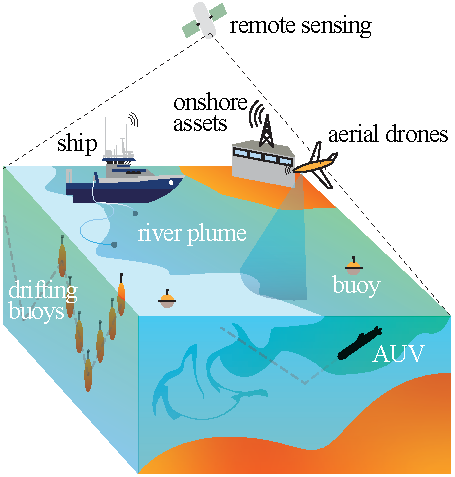
\includegraphics[width =
    0.49\textwidth]{Figures/envir.pdf}\label{fig:envir1}}
  \hfill
  \subfigure[Frontal patterns off of the Nidelva river, Trondheim, Norway.]{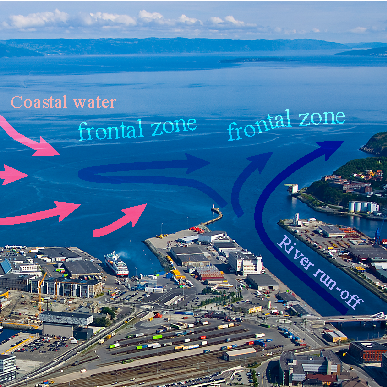
\includegraphics[width =
    0.49\textwidth]{Figures/river_proccess.pdf}\label{fig:nidelven}}
  \caption{\ref{fig:envir1} Traditional ocean observation based on 
    ship-based sampling has been augmented by autonomous
    robotic vehicles. % and their interactions.  
    AUV platforms are an integral part of this network being able to
    reason and make decisions for efficient onboard adaptive sampling.
    % using the sense-plan-act control approach to autonomous control. 
    \ref{fig:nidelven} The interaction of river and ocean creates
    processes that are challenging to map, where the combination of
    statistics and robotics can play a vital role in enabling more
    effective oceanographic observation.\kc{The inset ``AUV robot''
      looks very tacky and ad-hoc; might be best to remove it. Change
      ``ships'' to
      ``Ship'', remove the aerial drone, since we didn't use it and
      don't plan to in this work.}}
  \label{fig:envir} \end{figure}
%
\begin{comment} % Somehow redundant with the parag following below
Mobile robotic platforms \citep{Bellingham07} have contributed significantly to environmental monitoring and sampling. In particular, AUVs have advanced the state of in-situ sampling, and made robotics an integral part of ocean observation, filling parts of the undersampling gap \cite{rudnick03,rudnick18} (See Fig. \ref{fig:envir1}).
\end{comment}
%
The advent of robust mobile robotic platforms \citep{Bellingham07} has
resulted in significant contributions to environmental monitoring and
sampling in the ocean. In particular, autonomous underwater vehicles (AUVs) have advanced the state of data collection and consequently have made robotics an integral part of ocean observation; %our 
previous work by some of the authors of the present paper have contributed to this effort \citep{das11b,Das2015,fossuminformation,fossum18b}. 


As full numerical ocean models based on complex differential equations cannot be run onboard a marine robot with limited computational capacity, statistical models relying on collected data and random field assumptions appear quite relevant as means to guide AUV data collection trajectories. Our main research angle in the present work is to extend sequential design strategies from the world of spatial statistics and computer experiments to frameworks featuring both vector-valued observational data and experimental designs that may be constrained by the nature of feasible trajectories.      
\\

Surveys with AUVs are usually limited to observations along fixed
transects that are pre-scripted in mission plans created manually by a
human operator. Missions can be specified operating on a scale of
hundreds of meters to tens of kilometers depending on the scientific
context. Faced with limited coverage capacity, a more effective
approach is to instead use onboard algorithms to continuously
evaluate, update, and refine future sampling locations (sense-plan-act
cycle in Fig. \ref{fig:envir1}), making the information gathering
\emph{adaptive} \citep{das11b,Das2015,fossuminformation,fossum18b}.
% This usually occurs on a spatial grid, called a waypoint graph. 
In doing so, the space of sampling opportunities is still limited by
the so-called waypoint graph, a discretization of the search domain, but the AUV has flexibility to modify its path at each waypoint based on in-situ sensing and measurements onboard \citep{py10,Rajan12,Rajan12b}.\\

The work presented here is primarily inspired by a case study 
%application where an AUV is used to measure both temperature and salinity in 
pertaining to the spatial characterization of a frontal system generated by
river plumes. Fig. \ref{fig:nidelven} shows the survey area in
Trondheim, Norway, where cold freshwater enters from the river,
creating a strong gradient in both temperature and salinity. Because
of the local topography and the Coriolis force the cold fresh water
tends to flow to the east. Depending on the river discharge, tidal
effects, wind, and temperature differences, this boundary often gets
distorted. Initial knowledge about the location and evolution of these
features are highly uncertain, making deterministic planning
challenging. Here the goal is to use AUV measurements towards a better description of the interface between freshwater versus oceanic water, with the help of a vector-valued random field model for both temperature and salinity. As we will present in the next sections, some of the original contributions inspired by this specific problem are actually applicable to further settings and application areas. \\

The questions tackled here hence pertain to the broader area of spatial data collection and experimental design, yet with the particularity of estimating some regions of the domain, mostly excursion sets, being implicitly defined by a scarcely observed vector-valued random field. 
%because of limited resources to sample the large oceanographic domains, one must plan for active learning during the operation, where a relevant criterion is used to extract the most valuable designs. The acquired in-situ information must then be assimilated into the statistical model onboard the platform, so that it can be used to re-compute the sampling criterion and in this way inform decisions on where to sample next. \\
Moreover, given constraints on AUV movements and the fact that surveys rely by design in such a framework on successive measurements spread along a trajectory, addressing corresponding design problems calls for particular sequential strategies, possibly also accounting for the finiteness of resources by anticipating multiple steps ahead and thereby improving over myopic strategies. \\

Here we aim to leverage and extent recent progress in uncertainty quantification and reduction for excursion sets of Gaussian random fields in order to address vector-valued observational cases under constrained design such as in the motivating application of designing AUV trajectories to better distinguish between freshwater from ocean waters, relying on temperature and salinity measurements. %approach will take substantial advantage of existing work in the field of excursion set estimation mainly dedicated to computer experiments in the scalar-valued case, and where space exploration can be performed without constraints regarding the distance between successive design points. 
Original contributions compared to recent related work in the framework of scalar-valued (computer) experiments include: 
\begin{itemize}
    \item Extension of two important Sequential Uncertainty Reduction criteria of \citep{Bect.etal2012,chevalier2014fast,bect2019} to homotopic or heterotopic vector-valued settings,
    \item Investigation of myopic and multiple-step ahead batch-sequential strategies for optimizing trajectories with respect to such criteria,
    \item Replicable experiments with synthetic test cases and original data sets with accompagnying codes. 
\end{itemize}
Let us briefly review random field modelling and recent advances in targetd sequential design of experiments based on Gaussian Processes before detailing further existing literature tackling the considered problems, our proposed approach, as well as outlining the rest of the paper.  


\subsection{Random field modelling and targeted sequential design of experiments}
 
 While random field modelling has been one of the main topics throughout the history of spatial statistics \citep{Krige1951a, Matheron1963, Stein1999, Adler.Taylor2007}, there has recently been a renewed interest for random field models in the context of static sequential experimental design, be it in the context of spatial data collection \citep{Mueller2007} or in computer experiments and machine learning \citep[See for instance][and references therein]{Santner.etal2003, Romero.etal2013, Beck2016}. As detailed in \cite{Ginsbourger2018}, Gaussian random field models have been used in particular as a basis to sequential design of comupter experiments dedicated to various goals such as global optimization but also set estimation.  \cite{Picheny.etal2010} revisited the classical Integrated Mean Square Error criterion with an adaptation dedicated to contour line estimation, \cite{Bect.etal2012} focused on strategies to reduce uncertainties on volumes of excursion, i.e. on the measure of the domain of input parameters which associated (scalar) response level exceeds a prescribed threshold, followed up by \cite{chevalier2014fast} presenting computational contributions towards an efficient batch-sequential implementation of strategies introduced in the former. Meanwhile, rather than focusing on excursion volumes, some approaches were investigated in \cite{French.Sain2013,Chevalier.etal2013b,Bolin.Lindgren2015,Azzimonti.etal2016} that ambition to estimate sets themselves. Recently, sequential design of experiments for the conservative estimation of excursion sets based on Gaussian random field models was presented in \citep{Azzimonti.etal}. 
 %
Surprisingly less attention has been dedicated to sequential strategies in the case of vector-valued observations to our knowledge. It has been acknowledge for several decades that co-Kriging models could be efficiently updated with vector-valued observations being assimilated sequentially 
\cite{Vargas-Guzman1999}, sequential strategies targeted to estimate prescribed features of vector-valued random fields are not in still in their infancy. We can refer for instance to \citep{LeGratiet.etal2015} for co-Kriging-based sequential design using fast cross-validation and dedicated to multi-fidelity computer codes. Related ideas are to be found in \cite{Poloczek2017} in the context of Multi-Information Source Optimization. As for extensions of Stepwise Uncertainty Reduction strategies, to our knowledge the only attempt so far to generalize excursion-related Stepwise Uncertainty Reduction criteria (such as reviewed above) in vector-valued settings pertains to the design of multi-fidelity simulations for fire safety, in the PhD thesis \citep[][p.82]{stroh}, where the outputs are mainly assumed independent yet the feasibility of treating the dependent case by appealing to higher-dimensional Gaussian CDF evaluations is mentioned. 


% From earlier version; to be relocated?
%Hence statistical proxy models of the environment must be used. For our purpose, we rely on Gaussian process (GP) representations of the ocean variables of interest because they are computationally convenient and yet provide enough flexibility to realistically model the spatial variability and dependence, and the correlation between multiple processes. 
\subsection{Contributions, selected previous work on AUV sampling, and outline} 
%work and proposed approach in a nutshell}
%\begin{itemize}
%    \item 
%\end{itemize}
%\textcolor{blue}{We might want to re-use some of the following (from earlier version):}

A major contribution of our work is to derive closed-form results for
this design criteria for situations where the underlying model is
based on multivariate GPs. Another contribution is that we embed this
approach in a sequential strategy to produce sampling algorithms, and
apply this to a real-world scenario of autonomously sampling
temperature and salinity gradients using an AUV, with the intention of
characterizing the variability of oceanic and riverine waters in
typical mixed coastal environments.

Motivating examples relevant for ESs of multivariate processes are
abundant. In medicine, doctors do not rely solely on a single symptom
but must see several combined effects before making a diagnosis. In
our context of environmental sampling, the salinity and temperature
excursions of a river plume can similarly help characterize the
underlying bio-geochemical processes
\citep{hopkins2013detection,Pinto2018}, where sampling can be aimed
towards reducing uncertainty in the temperature and salinity ES.
Unlike what has been done in previous plume exploration studies, we
emphasize the links to spatial statistical modeling and targeted
multivariate sampling criteria for sequential sampling.

Other statistical
work in the oceanographic domain include \cite{wikle2013modern}
focusing on hierarchical statistical models; \cite{sahu2008space},
studying spatio-temporal models for sea surface temperature and
salinity data; and \cite{mellucci2018oceanic} looking at the
statistical prediction of features using an underwater glider.
In this paper the focus is not on statistical modeling, but rather on statistical results and computations for efficient sampling designs. 

We focus on spatial characterization of a frontal system generated by
river plumes. Fig. \ref{fig:nidelven} shows the survey area in
Trondheim, Norway, where cold freshwater enters from the river,
creating a strong gradient in both temperature and salinity. Because
of the local topography and the Coriolis force the cold fresh water
tends to flow to the east. Depending on the river discharge, tidal
effects, wind, and temperature differences, this boundary often gets
distorted. Initial knowledge about the location and evolution of these
features are highly uncertain, making deterministic planning
challenging.

Adaptive in-situ AUV sampling of an evolving frontal feature has been
explored in \cite{fronts11,Zhang2012,Pinto2018,costa19}. These
approaches typically use a reactive-adaptive scheme, whereby
exploration does not rely on a statistical model of the environment,
but rather adaptation is based on closing the sensing and actuation
loop. Myopic sampling, i.e. stage-wise selection of the path (on the
waypoint graph), has been used for surveys
\citep{singh2009efficient,Binney2013} that focus largely on reducing
predictive variance or entropy. These criteria are widely adopted in
the statistics literature on spatio-temporal design as well
\cite{bueso1998state,zidek2019monitoring}, but variance and entropy
reduction are independent of the actual data realizations under the
assumptions of GP models, so it has limited
decisional flexibility. The use of data-driven adaptive criteria
was introduced to include more targeted sampling of regions of
scientific interest in \cite{Low2009} and \cite{fossuminformation}. In
this paper, we focus on mapping the river plume by rewarding designs
that improve the classification of ES in temperature and salinity.

\begin{comment}
\subsection{Outline of the paper and its appendices / supplemental material}

\begin{itemize}
    \item 
\end{itemize}
\end{comment}

The remainder of this paper is organized as follows: 
%Section \ref{sec:bg} provides select background on ocean sampling. 
Section \ref{sec:ESEP} defines ESs, EPs, and the design criteria of IBV for
vector-valued GPs. Section \ref{sec:heuristics} builds on these
assumptions when deriving the sequential design criteria for adaptive
sampling. Section \ref{sec:simulations} discusses properties of the
methods in simulation studies. Section \ref{sec:case_study}
demonstrates the methodology used in field work characterizing a river
plume and finally, Section \ref{sec:concl_disc} contains a summary and
a discussion of future work.
%\section{Quantifying uncertainty on Excursion Sets implicitly defined by Gaussian processes}
\label{sec:ESEP}

In section \ref{sec:bg_and_notation} we introduce the notation used in the rest of the paper, review (co-)kriging of multivariate gaussian random fields (GRFs) and present update formulae for cokriging.
Uncertainty quantification (UQ) techniques on excursion sets of GRFs are presented in \ref{sec:set_uq}, in particular the Integrated Bernoulli Variance (IBV) and the excursion measure variance (EMV) are defined \textcolor{red}{and explicit expressions enabling their computation are derived.}
Section \ref{sec:eibv} turns to the effect of new observations on EMV and IBV. Specifically, the expected effect of the 
inclusion of a new set of observations on the EMV and IBV are considered and closed-form expressions for the expected 
uncertainty reduction are derived. Those expression form the backbone of the uncertainty reduction strategies presented in
Section \ref{sec:heuristics}.
Finally, Section \ref{Sec:UnivarEx} illustrates the application of the above concepts on a bivariate example relevant for 
sampling in the temperature and salinity application.

\medskip

Our objective is to leverage statistical tools onboard an autonomous
robotic platform to characterize a river plume, focusing on spatial
separation of cold freshwater from a river and warmer saline waters
of a fjord.

The temperature and salinity field over the domain of interest will be modeled as a bivariate gaussian random field. The \textcolor{red}{complement of the} river plume may then be characterized as an \textit{excursion set} of the field, that is, as the region of the domain for which temperature and salinity lie above some specified threshold. Our goal is then to guide the data collection process so as to improve the characterization of this set.
The methods we develop are fairly general, and not limited to the special case of two-dimensional random fields. Hence, the rest of this section will consider generic excursion sets of gaussian random fields with an arbitrary number of output dimensions.

\begin{figure}[h!] \centering
  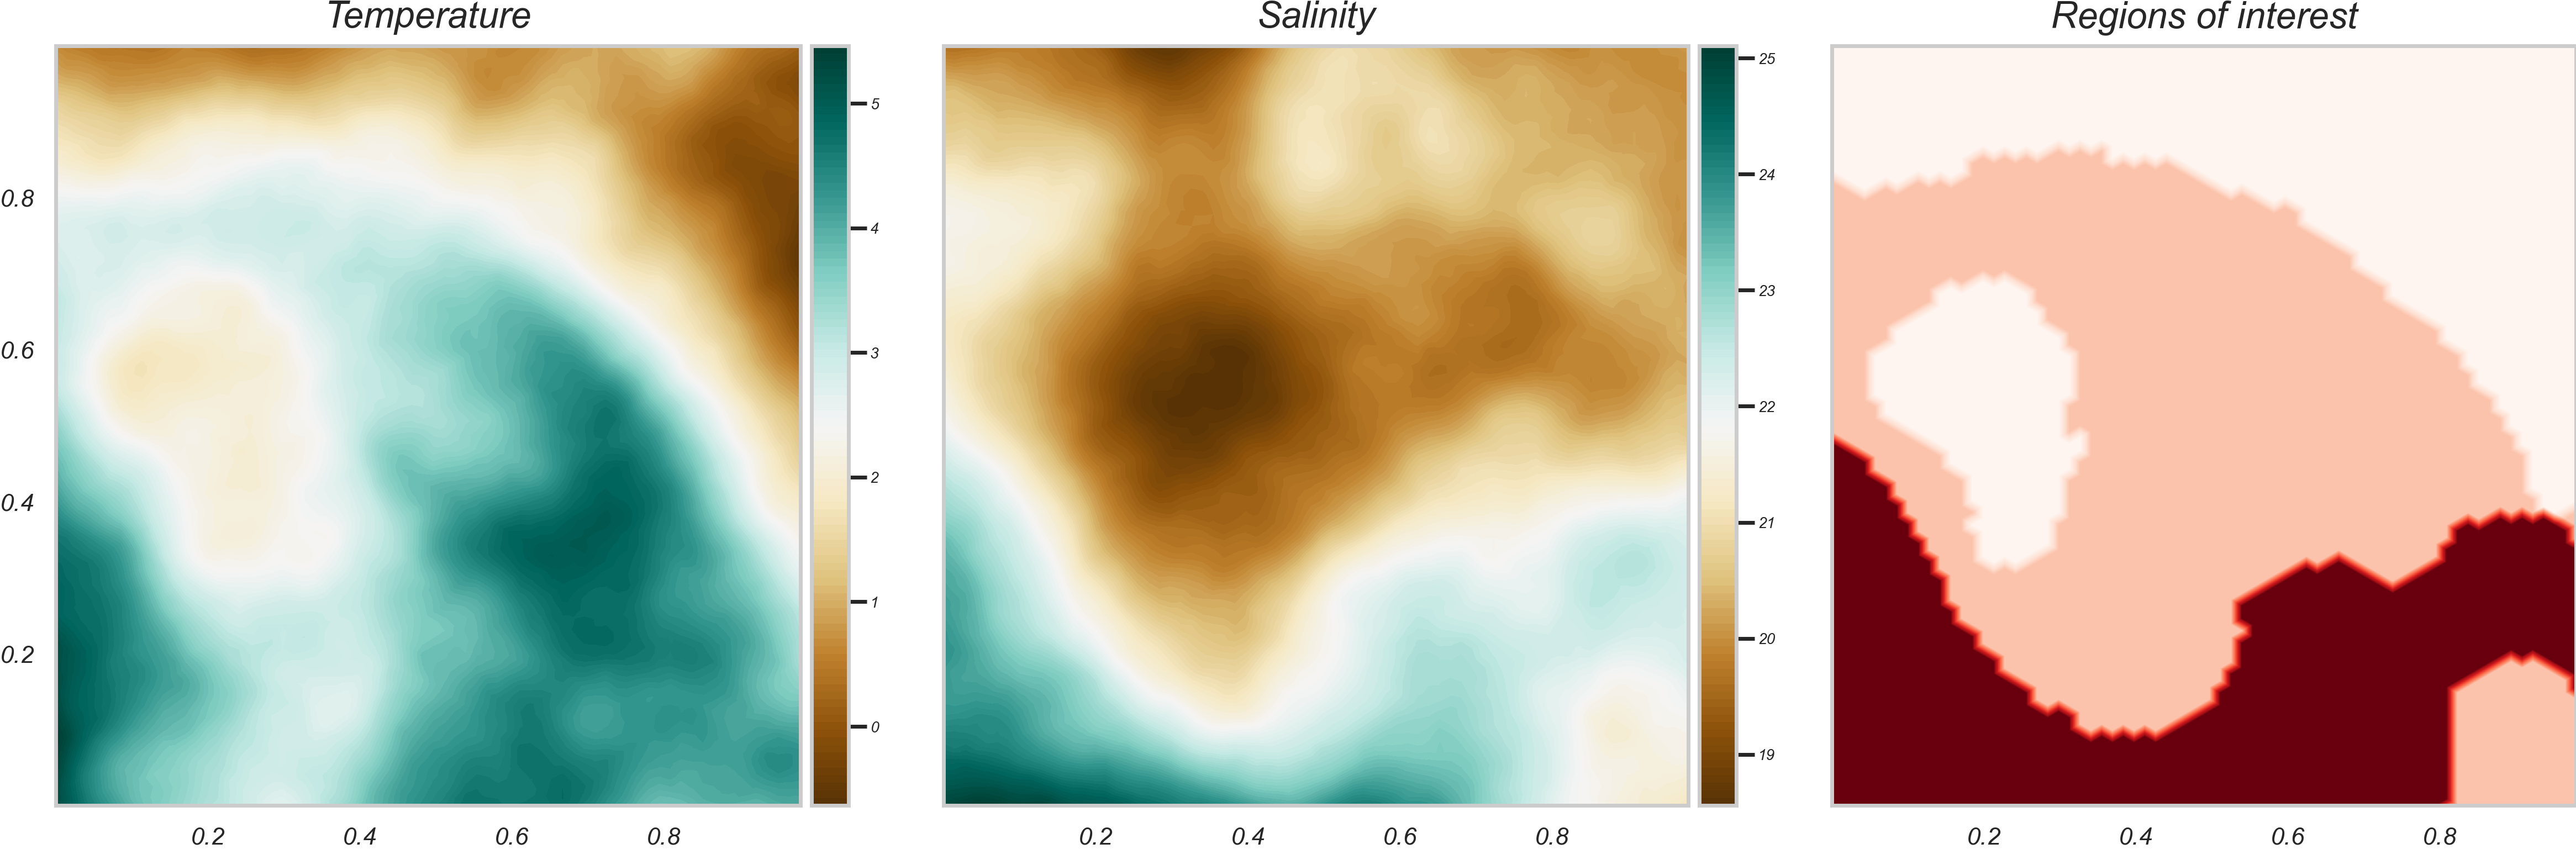
\includegraphics[width=0.99\textwidth]{Figures/example_excu_1.png}
  \caption{Realization of a bivariate GRF and excursion set above some threshold. Joint excursion in red, excursion of a single variable in white.}
\label{example_excu}
\end{figure}


Say we have an underlying phenomenon that is modeled as a $\no$-variate gaussian random field $\gp$ on some domain $\domain$, 
and we are interested in recovering the set of locations $\es$ in the domain for which the response variables (the components of $\gp$) lie in some set of specified values $\T\subset \mathbb{R}^{\no}$:
$$
\es:=\gp^{-1}(\T)=\{\x \in \mathcal{M}: \gp[\x] \in \T\}.
$$
Our goal here is to develop approaches to quantify and improve the
characterization of uncertainties on $\es$. \textcolor{red}{Alread mention how observations are included.}

If we assume that $\gp$ has
continuous trajectories (almost surely) and $T$ is closed, then
$\es$ becomes a Random Closed Set
\citep{Molchanov2005} and concepts from the theory of random sets will prove useful in characterizing the distribution of the volume of $\es$ under some measure defined on the domain.

\textcolor{red}{Is this really needed?} Note that while some aspects of the developed approaches do not call for a
specific form of $\T$, we will often stick for simplicity to the case
of orthants
($\T=(-\infty, t_1] \times \dots \times (-\infty, t_{\no}]$ where
$t_1,\dots, t_{\no} \in \R$) as this will allow efficient calculation
of several key quantities. Note that changing some $\leq$ inequalities
to $\geq$ ones would lead to immediate adaptations.


\subsection{Background, Notation and Co-Kriging}
\label{sec:bg_and_notation}
Given a random field $\gp$ and (noisy) observations of some of its components at some points in the domain, one can predict the value of the field at some unobserved location $\spatloc\in \domain$ by using the conditional mean of $\gp[\spatloc]$, conditional on the data. This process is called (co-)kriging, and kriging equations precisely tell us how to compute conditional means and covariances conditional on an arbitrary dataset.
We will here present the most general form of cokriging, where one can include several observations (batch) at a time and 
observations at a given location $s \in \domain$ may only include a subset of the components of $\gp[\spatloc]\in\mathbb{R}^{\no}$ 
(heterotopic).

\subsubsection{Notation}
In order to work at this level of generality, some notational tricks are needed. Indeed, when considering a new observation, one shall in general specify which component of the field was observed and where it was observed. This leads us to introduce the concept of \textit{generalized location}.

Letting $\gp[\spatloc,\ell]$ denote the $\ell\text{-th}$ component of $\gp[\spatloc]$, $\spatloc\in \domain$ and $\ell \in \{1\dots,p\}$, we will call \textit{generalized location} the couple $x=(\spatloc,\ell)$. Given such a generalized location notation $x$,  the notation $\gp[x]$ will be used to denote $\gp[\spatloc,\ell]$.

This slight change of notation will allow us to think of $\gp$ as a scalar-valued Gaussian random field 
indexed by $D\times \{1\dots,p\}$, which will give the co-kriging equations a particularly simple form that parallels the one of univariate kriging. Due to the naturality of the concept of \textit{generalized location}, 
we will generally use the word \textit{location}, while \textit{spatial location} will be used to stress that we are talking about a point $\spatloc \in \domain$. In the following, the letter $x$ will be reserved for generalized locations, while the letters $\spatloc$ and $\ell$ will be used for spatial locations and response indices respectively.

It turns out that the inclusion of several observations at a time (a batch) may be handled by the same equations as the 
one for a single observation, provided some notation adjustments are made. This motivates the following.



Given a dataset consisting of  $q$ observations at spatial locations $\spatloc_i \in \domain$ and response indices $l_i \in \lbrace 1, ..., \no\rbrace$, $i=1, ..., q$, we can concatenate the information needed to specify the dataset by using the notation
\begin{align*}
\bm{x}:=(\bm{\spatloc}, \bm{\ell}):= (x_1,\dots, x_q),~\text{with }x_i=(\spatloc_i,\ell_i).
\end{align*}
In general, boldface letters will be used to denote concatenated quantities corresponding to batches of observations. 
We can then also compactly denote the values of the field at those different locations by
\begin{align*}
\gp[\bm{x}]:=
\left(\gp[\spatloc_1,\ell_1], ...,
\gp[\spatloc_q,\ell_{q}]\right) \in \mathbb{R}^{q}.
\end{align*}
%
\subsubsection{Co-Kriging}
\label{sec:cokriging}
Assuming now that $n$ batches of observations are available, with respective sizes $q_1,\dots, q_n$, and that one wishes 
to predict $\gp[\bm{x}]$ for some batch of $q\geq 1$ generalized locations $\bm{x}=(\bm{\spatloc}, \bm{\ell})$, the (simple) 
cokriging mean would then amount to simple kriging with respect to a scalar-valued Gaussian random field indexed by 
$D\times \{1\dots,p\}$ and with covariance kernel $k(\bm{x}, \bm{x}')=K(\bm{\spatloc}, \bm{\spatloc}')_{\ell, \ell'}$, that is:
%
\begin{equation}
\mu_{[n]}(\bm{x})=\mu(\bm{x})+\lambda_{[n]}(\bm{x})^T (\mathbf{z}_{[n]}-\mu(\bm{x})),
\end{equation}
where $\mu$ is $Z$'s initial mean function, $\mathbf{z}_{[n]}$ stands for the ($\sum_{i=1}^n q_i$)-dimensional vector of 
observed responses of $Z$ at all considered generalized locations, and $\lambda_{[n]}(\bm{x})$ is a vector of weights 
equal to $k(\bm{x}_{[n]}, \bm{x}_{[n]})^{-1} k(\bm{x}_{[n]}, \bm{x})$ with $\bm{x}_{[n]}=(\bm{x}_1,\dots, \bm{x}_n)$, 
$k(\bm{x}_{[n]}, \bm{x}_{[n]})$ being assumed non-singular throughout the presentation. The co-kriging %(conditional) 
residual (cross-)covariance function (with respect to batches of generalized locations) can also be expressed in the same vein via
%
\begin{equation}
k_{[n]}(\bm{x},\bm{x}')=k(\bm{x},\bm{x}')-\lambda_{[n]}(\bm{x})^T k(\bm{x}_{[n]}, \bm{x}_{[n]}) \lambda_{{[n]}}(\bm{x}').
\end{equation}

\subsubsection{Co-kriging update formulae}

Let us now consider the case where co-kriging prediction of $Z$ was made with respect to $n$ batches $\bm{x}_i$ of generalized locations, concatenated again within
$\bm{x}_{[n]}=(\bm{x}_1,\dots, \bm{x}_n)$, and one wishes to update the prediction by incorporating a new vector of observations $\mathbf{z}_{n+1}$ measured at a batch of $q_{n+1} \geq 1$ generalized locations $\bm{x}_{n+1}$.
%It turns out that the concept of \textit{generalized location} makes the kriging formulae form-invariant across all dimensions. This allows us to directly adapt the 
Thanks to our representation of co-kriging in terms of simple kriging with respect to generalized locations, a strightforward adaptation of the batch-sequential kriging update formulae from \cite{Chevalier.etal2013a} delivers that
% 
\begin{equation}
\mu_{[n+1]}(\bm{x})=\mu_{[n]}(\bm{x})+\lambda_{[n+1,n+1]}(\bm{x})^T (\mathbf{z}_{n+1}-\mu(\bm{x}_{n+1})),
\end{equation}
where $\lambda_{[n+1,n+1]}(\bm{x})$ denotes the $q_{n+1}$-dimensional sub-vector extracted from
$\lambda_{[n+1]}(\bm{x})$ that corresponds to the kriging weigths associated with the last $q_{n+1}$ responses when 
predicting at $\bm{x}$ relying on all measurements until batch $(n+1)$.
%\text{th}$ batch.
%, i.e. those from the $(n+1)\text{th}$ batch of measurements conducted at $\bm{x}_{n+1}$.
Similarly, the updated co-kriging residual (cross-)covariance function then writes
\begin{equation}
k_{[n+1]}(\bm{x},\bm{x}')=k_{[n]}(\bm{x},\bm{x}')-\lambda_{[n+1,n+1]}(\bm{x})^T k_{[n]}(\bm{x}_{[n]}, \bm{x}_{[n]}) \lambda_{{[n+1,n+1]}}(\bm{x}').
\end{equation}
%\medskip
%
Let us remark that, as noted in \cite{Chevalier2015} in the case of scalar-valued fields, these update formulae naturally 
extend to Universal Kriging in second-order settings and apply without Gaussian assumption. We will now see how the latter formulae are instrumental in deriving semi-analytical formulae for stepwise uncertainty reduction criteria for 
vector-valued random fields.






\subsection{Uncertainty Quantification on Excursion Sets of multivariate Gaussian Random Fields}
\label{sec:set_uq}
We now introduce quantities that allow to quantify the uncertainty on the volume of the excursion set $\es$. Let $\mes$ be a 
(locally finite, Borel) measure  on $\domain$. We want to investigate the probability distribution 
of $\mes(\es)$ through its moments.

\medskip

Centred moments may be computed using Proposition~\ref{propo1} developed in the appendix. 
In particular, it allows to write the excursion measure variance $\emv = \operatorname{Var}[\mes(\es)]$ as an integral of the excursion probability
\begin{equation*}
\begin{split}
\emv
&=\int_{\domain^2} \mathbb{P}\left(
\gp[u]\in T, \gp[v]\in T \right)
d\mes^{\otimes}(u, v)\\
&-\left( \int_{\domain} \mathbb{P}\left(\gp[u]\in T\right) d\mes(u) \right)^2,
\end{split}
\end{equation*}
which boils down in the excursion/sojourn case where $\T=(-\infty, t_1] \times
\dots \times (-\infty, t_{\no}]$ to
\begin{equation*}
\begin{split}
\emv
%\operatorname{Var}[\mes(\es)]
&=\int_{\domain^2}
\varPhi_{2\no}
\left(
(\bt, \bt); \mu((u,v)),
K((u,v),(u,v))
\right)
\
\mathrm{d}\mes^{\otimes} %\mes
%\productMeasure
(u,v)\\
&-\left( \int_{\domain} \varPhi_{\no}\left(\bt;\mu(u), K(u)\right) d\mes(u) \right)^2,
\end{split}
\end{equation*}
%
Note that like in the case of scalar-valued fields, this quantity requires to work out an integral over $\domain^2$. In 
contrast, and still like in the scalar-valued case, the Integrated Bernoulli Variance (IBV) of \cite{Bect.etal} involves 
solely an integral on $\domain$ and can be expanded in our present settings as follows
\begin{equation*}
\begin{split}
\operatorname{IBV} %(\es) %;\mes)
&=\int_{\domain}
\mathbb{P}\left(\gp[\uu]\in T\right)(1-\mathbb{P}\left(\gp[\uu]\in T\right))
d\mes(u) \\
&=\int_{\domain}
\varPhi_{\no}\left(\bt;\mu(\uu), K(\uu)\right)
-\left(\varPhi_{\no}\left(\bt;\mu(\uu), K(\uu)\right) \right)^2
\mathrm{d}\mes(u).
\end{split}
\end{equation*}
%
Next we investigate uncertainty reduction criteria related to those indicators.






\subsection{Expected Integrated Bernoulli Variance and Excursion Measure}
\label{sec:eibv}
This section is devoted to computing the expected effect of the inclusion of new observations on the $\emv$ and $\ibv$ of the excursion set $\es$. Let us consider the same setting as in Section \ref{sec:cokriging} where $n$ batches of measurements have already been performed, and let 
$\currentExp{.}$ and $\currentProba{.}$ denote conditional expectation
and probability conditional on the first $n$ batches of observations, respectively. We want to co pute the effect of the inclusion of a new set of observations at $\bm{x}_{n+1}$ on the $\emv$ and $\ibv$.

For uncertainty functional such as $\ibv$ and $\emv$, we use a similar indexing system
with respect to a sequence of batch, and further indicate when applicable the new batch
of generalized location between parentheses; e.g., $\emv_{[n+1]}(\bm{x})$ denotes the value
of $\emv$ (a random variable, seen from ``step'' $n$, i.e. when knowing $Z$ solely at
the $n$ first generalized location batches) when adding observations at $\bm{x}$ to those
already available at step $n$.

\textcolor{red}{C.T.: This doesn't work, we cannot be that short on the definition of EIBV, it is highly unclear. I suggest we go for the following notation:
$$\operatorname{IBV}(\bm{x}; \bm{y})
$$ denotes the IBV under the current law of the field, conditioned on observing $\bm{y}$ at $\bm{x}$ (generalized, possibly batch observation). Then
$$
\operatorname{EIBV}(\bm{x}):=\mathbb{E}_{\bm{Y}}\left[\textrb{IBV}(\bm{x}; \bm{Y})\right]
$$
where $\bm{Y}$ is distributed according to the current law of $Z_{\bm{x}}$.}

\textcolor{red}{
The philosophy is the following: EIBV and EEMV are functionals of a probability distribution. Then, if not mentioned explicitly, the probability distribution will be taken to be the current law of the field. (This notation is highly efficient).}



\textcolor{red}{When one want to consider several steps, one can use $\textrm{IBV}_{n}(\bm{x}; \bm{y})$ to denote the fact that the starting point (starting probability distribution) is the law of the field at the $n$-th step $\mathbb{P}_n$ to which conditioning on $\bm{y}$ at $\bm{x}$ is added.}

\textcolor{red}{For a rigorous definition
$$
\operatorname{IBV}(\bm{x}; \bm{y}):=\int_{\domain}
\mathbb{P}\left(\gp[\uu]\in T\mid Z_{\bm{x}}=\bm{y}\right)(1-\mathbb{P}\left(\gp[\uu]\in T \mid Z_{\bm{x}}=\bm{y}\right))
d\mes(u) \\
$$
where $\mathbb{P}$ denotes the current law of the field.}



\begin{propo}
\label{propo_eibv}
Let $\eibv_{[n]}(\bm{x})=\currentExp{\ibv_{[n+1]}(\bm{x})}$ (where $\bm{x}$ plays
the role of $\bm{x}_{n+1}$) be the expected effect of adding an observation a $\bm{x}$ on the IBV.
Then we have
\begin{equation}
\begin{split}
\eibv_{[n]}(\bm{x})
&=\int_{D} \varPhi_{\no}\left(\bt;~\currentMean{\uu}, \currentCov{u, u}\right) d\mes(u)\\
&-\int_{D} \varPhi_{2\no}
\left(
\left(
\begin{matrix}
\bt-\currentMean{u}\\
\bt-\currentMean{u}
\end{matrix}
\right);
\mathbf{\Sigma}_{[n]}(\uu)
\right)
d\mes(u),
\end{split}
\end{equation}
where the matrix $\mathbf{\Sigma}_{[n]}(\uu)$ is defined as
\begin{equation*}
\begin{split}
\mathbf{\Sigma}_{[n]}(\uu)&=
\left(
\begin{matrix}
\currentCov{u, u} & \currentCov{u, u}-\futureCov{u, u}\\
\currentCov{u, u}-\futureCov{u, u} & \currentCov{u, u}
\end{matrix}
%\begin{matrix}
%\currentCov{u, u} & \Delta_{[n]}(\uu)\\
%\Delta_{[n]}(\uu) & \currentCov{u, u}
%\end{matrix}
\right).\\
\end{split}
\end{equation*}
\end{propo}

As for the expected excursion measure variance, a similar result may be derived.
\begin{propo}
\label{propo_emv}

\begin{equation*}
\begin{split}
\eemv_{[n]}(\bm{x})
&=\int_{D^2} 
\varPhi_{2\no}
\left(
(\bt, \bt); \mu((u,v)), 
K((u,v),(u,v))
\right) 
\
\mathrm{d}\mes^{\otimes} %\mes 
%\productMeasure 
(u,v)\\
&-\currentExp{
    \varPhi_{\no}\left(a_1+B_1 V; C_1\right)
    \varPhi_{\no}\left(a_2+B_2 V; C_2\right)
},
\end{split}
\end{equation*}

with $V=\gp[\bm{x}_{n+1}]-\currentMean{\bm{x}_{n+1}} \sim \mathcal{N}(0_{q_{n+1}},k_{[n]}(\bm{x}_{n+1},\bm{x}_{n+1}))$ and $a_1=\bt-\currentMean{\uu}$,
$B_1=-\lambda_{[n+1,n+1]}(\uu)^T$, $a_2=\bt-\currentMean{\vv}$, $B_2=-\lambda_{[n+1,n+1]}(\vv)^T$.

This integrand finally boils down to an evaluation of the $2\no$-dimensional Gaussian CDF by
Proposition~\ref{propo3}. Details are omitted here for brevity as we did not implement further
this criterion that requires numerical integration over $\domain^2$.
\end{propo}


Note that the calculation of the multivariate Gaussian cumulative distribution
may be done effectively using code such as that of
\cite{genz2009computation}. 

\textcolor{red}{Do we really want to keep this?}
A critical element in the derivation of a closed-form for the EIBV is
that the conditional mean in the cokriging equations is a linear
(affine) function of the data $\by_d$ and the covariance is not a
function of the data. This in turn means that the probabilities in Eq.
\eqref{eq:post_ep} involve inequality statements for linear
combinations of Gaussian variables. Related closed-form solutions have
been noted in similar contexts \citep{bhattacharjya2013value,
  chevalier2014fast,stroh}, but not generalized to our situation with
random sets for vector-valued GPs.











\subsection{Expected Bernoulli Variance on a two dimensional Example}
\label{Sec:UnivarEx}
We illustrate the EBV associated to different designs on a simple bivariate example. The example mimics our river plume application and hence the first and second component of the random field will be called \textit{temperature} and \textit{salinity} for illustrative purpose. Effects of the hyperparameters of the GRF prior on the excursion probabilities will also be studied. For simplicity, we begin with a \textit{pointwise} example, considering a single bivariate gaussian distribution (no spatiality).

\subsubsection{A pointwise study}
Say we want to study the excursion probability of a bivariate gaussian, where the excursion set is defined as
\[
\Gamma := \lbrace \spatloc \in \domain: Z_{\spatloc, 1} \geq t_1, Z_{\spatloc, 2}\geq t_2\rbrace
\]
and the thresholds are set equal to the mean; $\mu_1=t_1=5^o C$ for temperature and  $\mu_2=t_2=30$ mg/l for salinity, and we play with the temperature and salinity correlation and variances to study the effect on the EP and expected Bernoulli variance.

Fig. \ref{illus_bivarDens} shows contour plots of three different
densities with increasing correlation $\gamma$ between temperature and
salinity. 
\begin{figure}[h!] \centering
  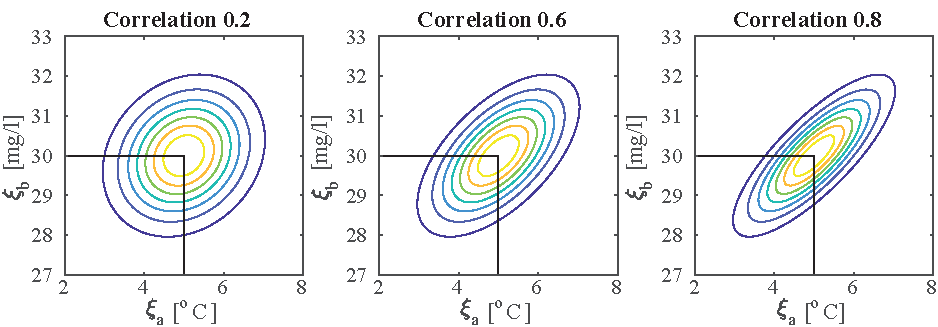
\includegraphics[width=0.99\textwidth]{Figures/illus_bivar.pdf}
  \caption{Density contour plots with different correlations between
    temperature and salinity. The densities have unit variance and the
    thresholds are identical to the mean values $5^o C$ and
    $30 mg/l$. X-axis is temperature and y-axis is salinity.}
\label{illus_bivarDens}
\end{figure}
The displayed densities have unit standard deviations for both
temperature and salinity, but we also study the effect of doubling the
standard deviations.

Table \ref{tab:sim_rhoab} shows the initial EPs and the associated
Bernoulli variance (second row) for the examples indicated in Fig.
\ref{illus_bivarDens}. The EPs increase with the correlation as there
is a strong tendency to have concurrently low temperature and salinity. The Bernoulli variance is similarly large for high
correlations. EPs and Bernoulli variances are the same for standard
deviation $1$ or $2$, which implies that high variability in
temperature and salinity is not captured in the $p(1-p)$ expression.

\begin{table}[!h] \centering \caption{EP and Bernoulli variance for
    different correlations and variances (top rows), and expected
    Bernoulli variances for both temperature and salinity data $\by$ and 
    temperature $y_2$ (bottom rows).}
  \begin{tabular}{c|ccc|ccc}
 &\multicolumn{3}{c}{$\sigma_1=\sigma_2=1$} & \multicolumn{3}{c}{$\sigma_1=\sigma_2=2$} \\
\hline
Correlation $\gamma$ & 0.2 & 0.6 & 0.8 & 0.2 & 0.6 & 0.8 \\
\hline
$p$ & 0.28 & 0.35 & 0.40 & 0.28 & 0.35 & 0.40 \\ 
$p(1-p)$ & 0.20 & 0.23 & 0.24 & 0.20 & 0.23 & 0.24 \\ 
EIBV, Temp and Salinity data & 0.092 & 0.089 & 0.085 & 0.052 & 0.051 & 0.049 \\ 
EIBV, Temperature data only & 0.151 & 0.138 & 0.123 & 0.137 & 0.114 & 0.093 \\ 
\hline
\end{tabular}
\label{tab:sim_rhoab}
\end{table}

Table \ref{tab:sim_rhoab} (bottom two rows) shows results of expected
Bernoulli variance calculations. This is presented for a design
gathering both data types, and for a design with temperature
measurements alone. When both data are gathered, the measurement model is
$(Y_{d,1},Y_{d,2})^t=(Z_1,Z_2)^t+\bepsilon$, with $\bepsilon \sim N(0,0.5^2I_2)$, while $Y_d=Z_1+\epsilon$, $\epsilon \sim N(0,0.5^2)$ when only temperature is measured.
For this illustration, Table \ref{tab:sim_rhoab} shows that the
expected Bernoulli variance gets lower with larger standard deviations
$\sigma_1$ and $\sigma_2$ (right columns). The reduction of Bernoulli
variance is largest for the cases with high correlation
$\gamma$. Albeit smaller, there is also uncertainty reduction when
only temperature is measured (bottom row), especially when temperature
and salinity are highly correlated. When correlation is low
($\gamma=0.2$), there is little information about salinity in the
temperature data, and therefore less uncertainty reduction. In an
application with fresh cold water from a river source, the temperature
and salinity variables will not only be interdependent, but will also
likely show dependence in the spatial dimension. This in turn will
impact the design criteria when we evaluate the information measure by
integrating over several locations (Section \ref{sec:simulations}).

\subsubsection{Including Spatiality}
INTRODUCTORY SENTENCE.
The class of GRF model we will consider in the article will generally have a linear trend
\begin{align*}
\mu(s)=\mathbb{E}\left[\begin{pmatrix}
Z_{s, 1}\\ Z_{s, 2}
\end{pmatrix}\right] &= \beta_0 + \beta_1 s
\end{align*}
with $\beta_0$ a two dimensional vector and $\beta_1$ a $2\times 2$ matrix. We will only consider covariance models of separable type
\begin{align*}
\textrm{Cov}\left(Z_{s, i}, Z_{u, j}\right) &= k(s, u) \gamma(i, j),~ \gamma(i, j) = \begin{cases} \sigma_l^2,~ i=j\\
   \gamma_0 \sigma_i \sigma_j,~i\neq j
        \end{cases}
\end{align*}
where $k(., .)$ is one of the traditional spatial covariance kernel (exponential, Mat\'{e}rn, ...) and $\gamma$ defines the cross-covariance structure.

In the accompanying Python code, these modeling assumptions can be
generalized to anisotropic covariance and changing variance levels
across the spatial domain. One can hence, easily run the code to see
if different models result in other sampling designs. Anisotropy and
non-stationary variance are both relevant for the setting with river
plumes, but in practice this requires more parameters to be
specified. With extensive data and prior knowledge, one could also
possibly fit and estimate parameters of more complex multivariate
spatial covariance functions
\citep{gneiting2010matern,genton2015cross}, but that is outside the
scope of the current paper.

In the rest of this section, we will consider a GRF with mean and covariance structure as above and parameters
\begin{align*}
\beta_0 = \begin{pmatrix}
5.8\\ 24.0
\end{pmatrix}, ~ \beta_1 = \begin{pmatrix}
0.0 & -4.0\\
0.0 & -3.8
\end{pmatrix},~ \sigma_1 = \sigma_2 = 2.25, ~ \gamma_0 = 0.2
\end{align*}
and the spatial covariance is given by a Mat\'{e}rn 3/2 kernel with unit variance and range parameter $\lambda=0.5$.
One realization of this GRF is shown in Fig. \ref{example_excu}.

We now study how the expected Bernoulli variance eq.\ref{eq:eibv} associated to data collection at a point changes if only one of the two components of the field is observed. We first draw a realization of the GRF defined above and use it as ground-truth to mimick the real data-collection process. A first data collection step is performed at the location in green, and the data is used to update the GRF model. The expected Bernoulli variance reduction (at each grid point) that would result from observing only one component, or both at the next grid point upwards is then computed an shown in Fig.\ref{fig:ebv_comp}.

\begin{figure}[h!] \centering
  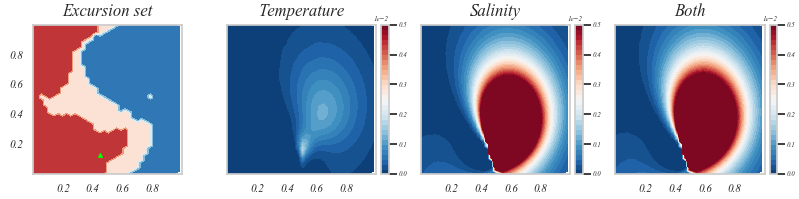
\includegraphics[width=0.99\textwidth]{Figures/ebv_comp.png}
  \caption{Pointwise Bernoulli variance reduction for observation of a single or both components of the random field at one location. Data collection locations in green. True excursion set in red. Places where only one response is above threshold are depicted in pink}
\label{fig:ebv_comp}
\end{figure}

Note that plotting the Bernoulli variance reduction at each point might also be used to compare different data collection plans. For example, Fig. \ref{fig:ebv_comp} shows the expected Bernoulli variance reduction associated to a data collection plan along a straight upwards line (static north) and the one associated to a straight horizontal line (static east). Both expectations are computed according to the a priori distribution of the GRF (i.e. no observations have been included yet).

\begin{figure}[h!] \centering
  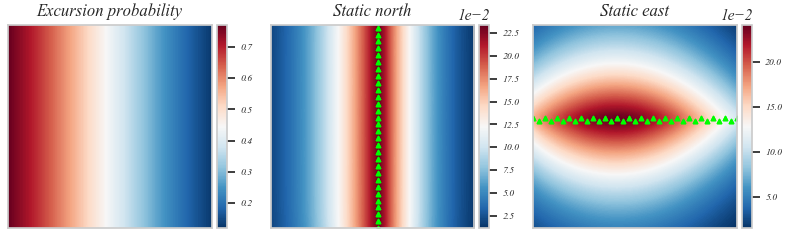
\includegraphics[width=0.99\textwidth]{Figures/ebv_north_vs_east.png}
  \caption{Pointwise Bernoulli variance reduction for two different observation plans. Data collection locations in green. True excursion set is in red. Places where only one response is above threshold are depicted in pink.}
\label{fig:ebv_north_vs_east}
\end{figure}

\begin{remark}
In all the above examples, the spatial domain $\domain$ has been discretized to a set of $n$ grid
locations $\mathcal{M}_g = \{\x_i, i=1,\ldots,n \}$, where each cell
has area $\Delta$; the same grid is used for the waypoint graph for
possible design locations. The EIBV is approximated by sums over all
grid cells.
\end{remark}





\section{Quantifying uncertainty on Excursion Sets implicitly defined by Gaussian processes}
\label{sec:ESEP}

In section \ref{sec:bg_and_notation} we introduce the notation used in the rest of the paper, review (co-)kriging of multivariate gaussian random fields (GRFs) and present update formulae for cokriging.
Uncertainty quantification (UQ) techniques on excursion sets of GRFs are presented in \ref{sec:set_uq}, in particular the Integrated Bernoulli Variance (IBV) and the excursion measure variance (EMV) are defined and semi-analytical expressions easing their computation and optimization are derived.
Section \ref{sec:eibv} turns to the  effect of new observations on EMV and IBV. Specifically, the expected effect of the inclusion of a new set of observations on the EMV and IBV are considered and further semi-analytical expressions for the expected 
uncertainty reduction are derived. The resulting formulae form the backbone of the uncertainty reduction strategies presented in Section \ref{sec:heuristics}.
Finally, Section \ref{Sec:UnivarEx} illustrates the application of the above concepts on a bivariate example relevant for sampling in the temperature and salinity application.

\subsection{Background, Notation and Co-Kriging}
\label{sec:bg_and_notation}

Throughout the rest of the article, we denote by $\gp$ a vector-valued random field indexed by some arbitrary domain $\domain$, and assume values of the field at any fixed location $\x \in \domain$, denoted $\gp[\x]$, to be a $\no$-variate random vector ($\no\geq 2$). In our leading river plume characterization application, $\domain$ is a prescribed domain in the fjord of Trondheim (for the purpose of our AUV application, a discretization of a $2$-dimensional domain at fixed depth is considered), while $\no=2$ and the two responses of interest stand for temperature and salinity. A bivariate gaussian random field model is assumed for $\gp$, see the two first panels of Figure~\ref{example_excu} for an illustration of a realization of such a vector-valued model (RK NOTATION). The right panel of this figure represents a by-product of interest derived from these realizations, namely regions i) in red, where both temperature and salinity are high (i.e., exceeding respective thresholds), standing for ocean water ii) in pink, where both temperature and salinity are low, standing for riverine water, and iii) in white, where one variable is above and the other below their respective thresholds, standing for mixed waters. 

\begin{figure}[h!] \centering
  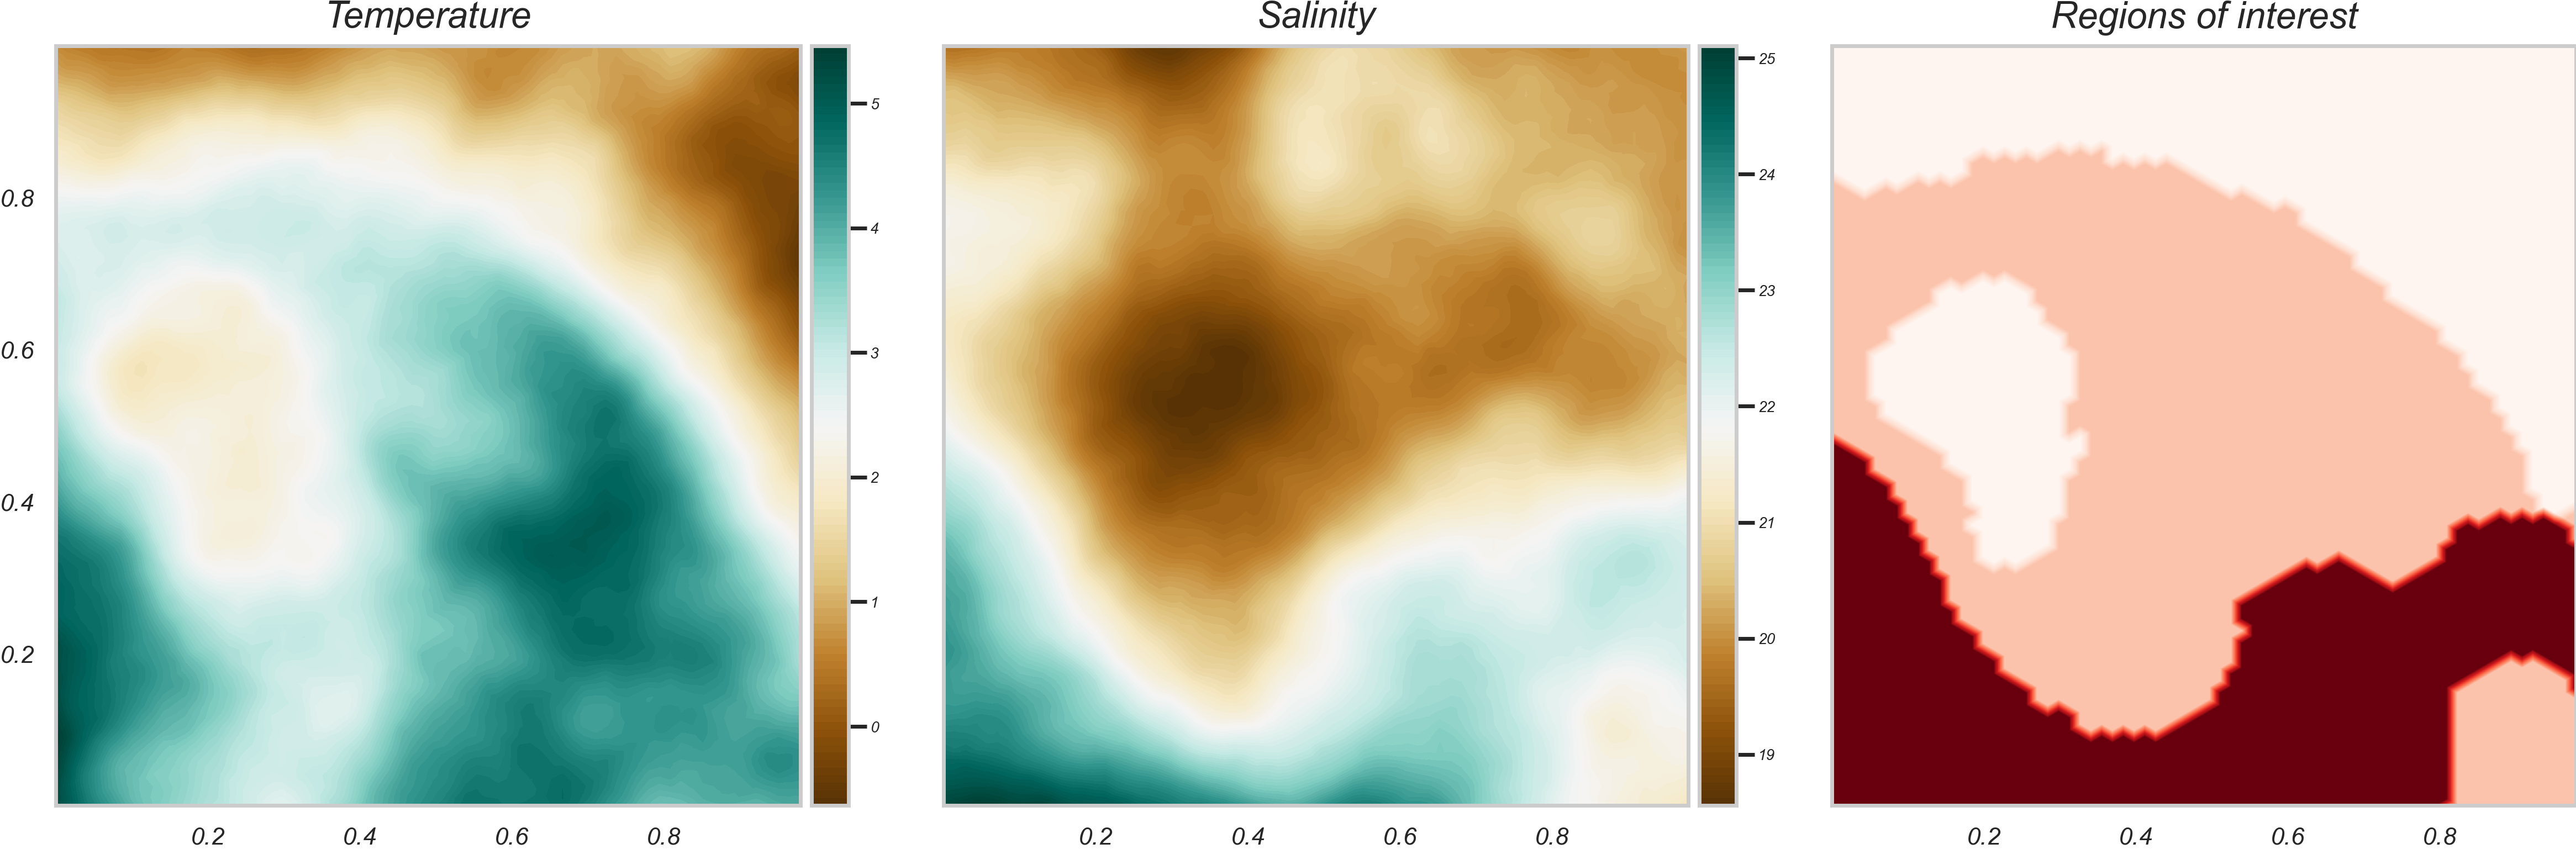
\includegraphics[width=0.99\textwidth]{Figures/example_excu_1.png}
  \caption{Realization of a bivariate GRF and excursion set above some threshold. Joint excursion in red, excursion of a single variable in pink.}
\label{example_excu}
\end{figure}

%The methods we develop are fairly general, and not limited to the special case of two-dimensional random fields. Hence, the rest of this section will consider generic excursion sets of gaussian random fields with an arbitrary number of output dimensions.
% Say we have an underlying phenomenon that is modeled as a $\no$-variate gaussian random field $\gp$ on some domain $\domain$, 
Coming back to the more general settings of a $\no$-variate random field, 
we are interested in recovering the set of locations $\es$ in the domain for which the response variables (the components of $\gp$) lie in some set of specified values $\T\subset \mathbb{R}^{\no}$, in other words \textit{the pre-image of $T$ by $\gp$}:
$$
\es:=\gp^{-1}(\T)=\{\x \in \mathcal{M}: \gp[\x] \in \T\}.
$$
%
%Our goal here is to develop approaches to quantify and improve the
%characterization of uncertainties on $\es$. \textcolor{red}{Alread mention how observations are included.}

If we assume that $\gp$ has
continuous trajectories (almost surely) and $T$ is closed, then
$\es$ becomes a Random Closed Set
\citep{Molchanov2005} and concepts from the theory of random sets will prove useful in characterizing the distribution of the volume of $\es$ under some measure defined on the domain.
%\textcolor{red}{Is this really needed?} 
Note that while some aspects of the developed approaches do not call for a
specific form of $\T$, we will often stick for simplicity to the case
of orthants
($\T=(-\infty, t_1] \times \dots \times (-\infty, t_{\no}]$ where
$t_1,\dots, t_{\no} \in \R$) as this will allow efficient calculation
of several key quantities. Note that changing some $\leq$ inequalities
to $\geq$ ones would lead to immediate adaptations.

\medskip

%\subsubsection{Notation}
%In order to work at this level of generality, some notational tricks are needed. Indeed, when considering a new observation, one shall in general specify which component of the field was observed and where it was observed. This leads us to introduce the concept of \textit{generalized location}.

Letting $\gp[\spatloc,\ell]$ denote the $\ell\text{-th}$ component of $\gp[\spatloc]$, $\spatloc\in \domain$ and $\ell \in \{1\dots,p\}$, we will call \textit{generalized location} the couple $x=(\spatloc,\ell)$. 
%Given such a generalized location notation $x$,  
The notation $\gp[x]$ will be used to denote $\gp[\spatloc,\ell]$ 
and
%
%This slight change of notation 
will allow us to think of $\gp$ as a scalar-valued %Gaussian 
random field indexed by $D\times \{1\dots,p\}$, which will give the co-kriging equations a particularly simple form that parallels the ones of kriging for the scalar-valued case. 
%Due to the naturality of the concept of \textit{generalized location},  we will generally use the word \textit{location}, while \textit{spatial location} will be used to stress that we are talking about a point $\spatloc \in \domain$. 
In the following, the letter $x$ will be reserved for generalized locations, while the letters $\spatloc$ and $\ell$ will be used for \textit{spatial locations} and \textit{response indices}, respectively.

It turns out that the inclusion of several observations at a time (a batch) may be handled by the same equations as the 
one for a single observation, provided some notation adjustments are made. This motivates the following.Given a dataset consisting of  $q$ observations at spatial locations $\spatloc_i \in \domain$ and response indices $\ell_i \in \lbrace 1, ..., \no\rbrace$, $i=1, ..., q$, we can concatenate the information needed to specify the dataset by using the notation
\begin{align*}
\bm{x}:=%(\bm{\spatloc}, \bm{\ell}):= 
(x_1,\dots, x_q),~\text{with }x_i=(\spatloc_i,\ell_i).
\end{align*}
In general, boldface letters will be used to denote concatenated quantities corresponding to batches of observations. 
We can then also compactly denote the values of the field at those different locations by
\begin{align*}
\gp[\bm{x}]:=
\left(\gp[\spatloc_1,\ell_1], ...,
\gp[\spatloc_q,\ell_{q}]\right) \in \mathbb{R}^{q}.
\end{align*}
%
For a second order random field $(Z_{\spatloc})_{\spatloc \in \domain}$ with mean $\mu$ and matrix covariance function $K$, $\mu$ is naturally extended to $\domain \in \lbrace 1, ..., \no\rbrace$ into a function of $x=(\spatloc, \ell)$ and is further straightforwardly vectorized into a function of $\bm{x}$. As for $K$, it induces a covariance kernel $k$ on the set of extended locations via  $k((\spatloc, \ell),(\spatloc', \ell'))=K(\spatloc, \spatloc')_{\ell, \ell'}$. In vectorized/batch form, $k(\bm{x}, \bm{x}')$ then amounts to a matrix with numbers of lines and columns the numbers of generalized locations in the batches $\bm{x}$ in $\bm{x}'$, respectively. Such vectorized quantities will turn out to be quite useful in order to arrive at embarrassingly simple expressions for co-Kriging equations below.  
%\textcolor{red}{(ADDENDUM, C.T.) In the same fashion, we will use $\mu(\bm{x})$ to denote the $q$-dimensional vector corresponding to the mean at $\bm{x}$ and $k(\bm{x}, \bm{x})$ for the corresponding $q \times q$ covariance matrix.}



Now given a Gaussian random field $\gp$ and (noisy) observations of some of its components at some points in the domain, one can predict the value of the field at some unobserved location $\spatloc\in \domain$ by using the conditional mean of $\gp[\spatloc]$, conditional on the data. This process is called (co-)kriging, and kriging equations precisely tell us how to compute conditional means and covariances conditional on an arbitrary dataset.
We will here present a rather general form of cokriging, in the sense that it allows including several observations (batch) at a time and 
observations at a given location $s \in \domain$ may only include a subset of the components of $\gp[\spatloc]\in\mathbb{R}^{\no}$ 
(heterotopic).

\subsubsection{Co-Kriging}
\label{sec:cokriging}
% Adressed during a discussion on 19.06.2020
%\textcolor{red}{(C.T.) Why mention batches? We do not care. We have previously available data at $\bm{x}$ and want to predict at $\bm{x}$'. No need to introduce concepts we will never use. Moreover, this presentation suggest that to go from n to n+1 (batch-) observations, we have to condition on the whole $n$ dataset, instead of only including the last step.}

Assuming that $n$ batches of observations are available, with respective sizes $q_1,\dots, q_n$, and that one wishes 
to predict $\gp[\bm{x}]$ for some batch of $q\geq 1$ generalized locations $\bm{x}$, %\equiv(\bm{\spatloc}, \bm{\ell})$, 
the (simple) cokriging mean would then amount to simple kriging with respect to a scalar-valued Gaussian random field indexed by 
$D\times \{1\dots,p\}$:  
%and with covariance kernel $k(\bm{x}, \bm{x}')=K(\bm{\spatloc}, \bm{\spatloc}')_{\ell, \ell'}$, that is:
%
\begin{equation}\label{eq:cokrig_mean}
\mu_{[n]}(\bm{x})=\mu(\bm{x})+\lambda_{[n]}(\bm{x})^T (\mathbf{z}_{[n]}-\mu(\bm{x})),
\end{equation}
where $\mu$ is $Z$'s initial mean function, $\mathbf{z}_{[n]}$ stands for the ($\sum_{i=1}^n q_i$)-dimensional vector of 
observed responses of $Z$ at all considered generalized locations, and $\lambda_{[n]}(\bm{x})$ is a vector of weights 
equal to $k(\bm{x}_{[n]}, \bm{x}_{[n]})^{-1} k(\bm{x}_{[n]}, \bm{x})$ with $\bm{x}_{[n]}=(\bm{x}_1,\dots, \bm{x}_n)$, 
$k(\bm{x}_{[n]}, \bm{x}_{[n]})$ being assumed non-singular throughout the presentation. The co-kriging %(conditional) 
residual (cross-)covariance function (with respect to batches of generalized locations) can also be expressed in the same vein via
%
\begin{equation}\label{eq:cokrig_cov}
k_{[n]}(\bm{x},\bm{x}')=k(\bm{x},\bm{x}')-\lambda_{[n]}(\bm{x})^T k(\bm{x}_{[n]}, \bm{x}_{[n]}) \lambda_{{[n]}}(\bm{x}').
\end{equation}

\subsubsection{Co-kriging update formulae}

Let us now consider the case where co-kriging prediction of $Z$ was made with respect to $n$ batches $\bm{x}_i$ of generalized locations, concatenated again within
$\bm{x}_{[n]}=(\bm{x}_1,\dots, \bm{x}_n)$, and one wishes to update the prediction by incorporating a new vector of observations $\mathbf{z}_{n+1}$ measured at a batch of $q_{n+1} \geq 1$ generalized locations $\bm{x}_{n+1}$.
%It turns out that the concept of \textit{generalized location} makes the kriging formulae form-invariant across all dimensions. This allows us to directly adapt the 
Thanks to our representation of co-kriging in terms of simple kriging with respect to generalized locations, a strightforward adaptation of the batch-sequential kriging update formulae from \cite{Chevalier.etal2013a} delivers that
% 
\begin{equation}
\mu_{[n+1]}(\bm{x})=\mu_{[n]}(\bm{x})+\lambda_{[n+1,n+1]}(\bm{x})^T (\mathbf{z}_{n+1}-\mu(\bm{x}_{n+1})),
\end{equation}
where $\lambda_{[n+1,n+1]}(\bm{x})$ denotes the $q_{n+1}$-dimensional sub-vector extracted from
$\lambda_{[n+1]}(\bm{x})$ that corresponds to the kriging weigths associated with the last $q_{n+1}$ responses when 
predicting at $\bm{x}$ relying on all measurements until batch $(n+1)$.
%\text{th}$ batch.
%, i.e. those from the $(n+1)\text{th}$ batch of measurements conducted at $\bm{x}_{n+1}$.
Similarly, the updated co-kriging residual (cross-)covariance function then writes
\begin{equation}
k_{[n+1]}(\bm{x},\bm{x}')=k_{[n]}(\bm{x},\bm{x}')-\lambda_{[n+1,n+1]}(\bm{x})^T k_{[n]}(\bm{x}_{[n]}, \bm{x}_{[n]}) \lambda_{{[n+1,n+1]}}(\bm{x}').
\end{equation}
%\medskip
%
Let us remark that, as noted in \cite{Chevalier2015} in the case of scalar-valued fields, these update formulae naturally 
extend to Universal Kriging in second-order settings and apply without Gaussian assumption. We will now see how the latter formulae are instrumental in deriving semi-analytical formulae for stepwise uncertainty reduction criteria for 
vector-valued random fields.






\subsection{Uncertainty Quantification on Excursion Sets of multivariate Gaussian Random Fields}
\label{sec:set_uq}
We now introduce quantities that allow to quantify the uncertainty on the volume of the excursion set $\es$. Let $\mes$ be a 
(locally finite, Borel) measure  on $\domain$. We want to investigate the probability distribution 
of $\mes(\es)$ through its moments.

\medskip

Centred moments may be computed using Proposition~\ref{propo1} developed in the appendix. 
In particular, it allows to write the excursion measure variance $\emv = \operatorname{Var}[\mes(\es)]$ as an integral of the excursion probability
\begin{equation*}
\begin{split}
\emv
&=\int_{\domain^2} \mathbb{P}\left(
\gp[u]\in T, \gp[v]\in T \right)
d\mes^{\otimes}(u, v)\\
&-\left( \int_{\domain} \mathbb{P}\left(\gp[u]\in T\right) d\mes(u) \right)^2,
\end{split}
\end{equation*}
which boils down in the excursion/sojourn case where $\T=(-\infty, t_1] \times
\dots \times (-\infty, t_{\no}]$ to
\begin{equation*}
\begin{split}
\emv
%\operatorname{Var}[\mes(\es)]
&=\int_{\domain^2}
\varPhi_{2\no}
\left(
(\bt, \bt); \mu((u,v)),
K((u,v),(u,v))
\right)
\
\mathrm{d}\mes^{\otimes} %\mes
%\productMeasure
(u,v)\\
&-\left( \int_{\domain} \varPhi_{\no}\left(\bt;\mu(u), K(u)\right) d\mes(u) \right)^2,
\end{split}
\end{equation*}
%
Note that like in the case of scalar-valued fields, this quantity requires to work out an integral over $\domain^2$. In 
contrast, and still like in the scalar-valued case, the Integrated Bernoulli Variance (IBV) of \cite{bect2019} involves 
solely an integral on $\domain$ and can be expanded in our present settings as follows
\begin{equation*}
\begin{split}
\operatorname{IBV} %(\es) %;\mes)
&=\int_{\domain}
\mathbb{P}\left(\gp[\uu]\in T\right)(1-\mathbb{P}\left(\gp[\uu]\in T\right))
d\mes(u) \\
&=\int_{\domain}
\varPhi_{\no}\left(\bt;\mu(\uu), K(\uu)\right)
-\left(\varPhi_{\no}\left(\bt;\mu(\uu), K(\uu)\right) \right)^2
\mathrm{d}\mes(u).
\end{split}
\end{equation*}
%
Next we investigate uncertainty reduction criteria related to those indicators.






\subsection{Expected Integrated Bernoulli Variance and Excursion Measure}
\label{sec:eibv}
This section is devoted to computing the expected effect of the inclusion of new observations on the $\emv$ and $\ibv$ of the excursion set $\es$. Let us consider the same setting as in Section \ref{sec:cokriging} where $n$ batches of measurements have already been performed, and let 
$\currentExp{.}$ and $\currentProba{.}$ denote conditional expectation
and probability conditional on the first $n$ batches of observations, respectively. We want to compute the effect of the inclusion of a new set of observations at $\bm{x}_{n+1}$ on the $\emv$ and $\ibv$.


For uncertainty functional such as $\ibv$ and $\emv$, we use a similar indexing system
with respect to a sequence of batch and use $\IBV_{\stage}$ to denote $\IBV$ with respect to the conditional law $\mathbb{P}_{\stage}$.

\medskip

In order to study the effect of the inclusion of a new data point, we let
$
\currentIBV(\bm{x}; \bm{y})
$
denote the IBV under the current law of the field, conditioned on observing $\bm{y}$ at $\bm{x}$ (generalized, possibly batch observation). The expected effect of a new observation on the IBV is then captured by
\begin{equation}\label{def:eibv}
    \currentEIBV(\bm{x}):=\mathbb{E}_{\stage}\left[\textrb{IBV}(\bm{x}; \bm{Y})\right]
\end{equation}
where $\bm{Y}$ is distributed according to the current law of $Z_{\bm{x}}$.


\textcolor{red}{
The philosophy is the following: EIBV and EEMV are functionals of a probability distribution. Then, if not mentioned explicitly, the probability distribution will be taken to be the current law of the field. (This notation is highly efficient).}


We next present a result that allows to compute $\EIBV$ as an integral of CDFs of multivariate gaussians. This will prove useful when designing sequential uncertainty reduction strategies.

\begin{propo}
\label{propo_eibv}
\begin{equation}
\begin{split}
\currentEIBV(\bm{x})
&=\int_{D} \varPhi_{\no}\left(\bt;~\currentMean{\uu}, \currentCov{u, u}\right) d\mes(u)\\
&-\int_{D} \varPhi_{2\no}
\left(
\left(
\begin{matrix}
\bt-\currentMean{u}\\
\bt-\currentMean{u}
\end{matrix}
\right);
\mathbf{\Sigma}_{[n]}(\uu)
\right)
d\mes(u),
\end{split}
\end{equation}
where the matrix $\mathbf{\Sigma}_{[n]}(\uu)$ is defined as
\begin{equation*}
\begin{split}
\mathbf{\Sigma}_{[n]}(\uu)&=
\left(
\begin{matrix}
\currentCov{u, u} & \currentCov{u, u}-\futureCov{u, u}\\
\currentCov{u, u}-\futureCov{u, u} & \currentCov{u, u}
\end{matrix}
%\begin{matrix}
%\currentCov{u, u} & \Delta_{[n]}(\uu)\\
%\Delta_{[n]}(\uu) & \currentCov{u, u}
%\end{matrix}
\right).\\
\end{split}
\end{equation*}
\end{propo}

As for the expected excursion measure variance, a similar result may be derived.
\begin{propo}
\label{propo_emv}

\begin{equation*}
\begin{split}
\eemv_{[n]}(\bm{x})
&=\int_{D^2} 
\varPhi_{2\no}
\left(
(\bt, \bt); \mu((u,v)), 
K((u,v),(u,v))
\right) 
\
\mathrm{d}\mes^{\otimes} %\mes 
%\productMeasure 
(u,v)\\
&-\currentExp{
    \varPhi_{\no}\left(a_1+B_1 V; C_1\right)
    \varPhi_{\no}\left(a_2+B_2 V; C_2\right)
},
\end{split}
\end{equation*}

with $V=\gp[\bm{x}_{n+1}]-\currentMean{\bm{x}_{n+1}} \sim \mathcal{N}(0_{q_{n+1}},k_{[n]}(\bm{x}_{n+1},\bm{x}_{n+1}))$ and $a_1=\bt-\currentMean{\uu}$,
$B_1=-\lambda_{[n+1,n+1]}(\uu)^T$, $a_2=\bt-\currentMean{\vv}$, $B_2=-\lambda_{[n+1,n+1]}(\vv)^T$.

This integrand finally boils down to an evaluation of the $2\no$-dimensional Gaussian CDF by
Proposition~\ref{propo3}. Details are omitted here for brevity as we did not implement further
this criterion that requires numerical integration over $\domain^2$.
\end{propo}


Note that the calculation of the multivariate Gaussian cumulative distribution
may be done effectively using code such as that of
\cite{genz2009computation}. 

\begin{remark}
Propositions \ref{propo_eibv} and \ref{propo_emv} are twofold generalizations of  results from \cite{chevalier2014fast}: they extend previous results to the multivariate setting and also allow for the inclusion of batch or heterotopic observations through the concept of generalized locations. Related closed-form solutions have been noted in similar contexts \citep{bhattacharjya2013value,stroh}, but not generalized to our situation with
random sets for vector-valued GPs.
\end{remark}












\subsection{Expected Bernoulli Variance on a two dimensional Example}
\label{Sec:UnivarEx}

We illustrate the EBV associated to different designs on a simple bivariate example. The example mimics our river plume application and hence the first and second component of the random field will be called \textit{temperature} and \textit{salinity} for illustrative purpose. Effects of the hyperparameters of the GRF prior on the excursion probabilities will also be studied. For simplicity, we begin with a \textit{pointwise} example, considering a single bivariate gaussian distribution (no spatiality).

\subsubsection{A pointwise study}
\textcolor{red}{(C.T.) What is EIBV in the table? How can we take an integral here? Also note that if we keep the ellipsoid plots, they should have Z's instead of Xi's}


Say we want to study the excursion probability of a bivariate gaussian above some thresholds, where the thresholds are set equal to the mean; $\mu_1=t_1=5^o C$ for temperature and  $\mu_2=t_2=30$ mg/l for salinity, and we play with the temperature and salinity correlation and variances to study the effect on the EP and expected Bernoulli variance.

% To BE COMMENTED (TEMPORARILY?)
Fig. \ref{illus_bivarDens} shows contour plots of three different
densities with increasing correlation $\gamma$ between temperature and
salinity. 
\begin{figure}[h!] \centering
  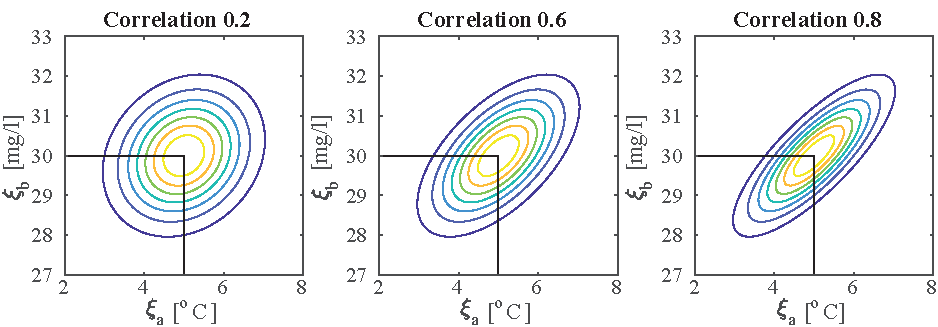
\includegraphics[width=0.99\textwidth]{Figures/illus_bivar.pdf}
  \caption{Density contour plots with different correlations between
    temperature and salinity. The densities have unit variance and the
    thresholds are identical to the mean values $5^o C$ and
    $30 mg/l$. X-axis is temperature and y-axis is salinity.}
\label{illus_bivarDens}
\end{figure}
The displayed densities have unit standard deviations for both
temperature and salinity, but we also study the effect of doubling the
standard deviations.
% END TO BE COMMENTED (TEMPORARILY?)

Table \ref{tab:sim_rhoab} shows the initial EPs and the associated
Bernoulli variance (second row) for the examples indicated in Fig.
\ref{illus_bivarDens}. The EPs increase with the correlation as there
is a strong tendency to have concurrently low temperature and salinity. The Bernoulli variance is similarly large for high
correlations. EPs and Bernoulli variances are the same for standard
deviation $1$ or $2$, which implies that high variability in
temperature and salinity is not captured in the $p(1-p)$ expression.

\begin{table}[!h] \centering \caption{EP and Bernoulli variance for
    different correlations and variances (top rows), and expected
    Bernoulli variances for both temperature and salinity data $\by$ and 
    temperature $y_2$ (bottom rows).}
  \begin{tabular}{c|ccc|ccc}
 &\multicolumn{3}{c}{$\sigma_1=\sigma_2=1$} & \multicolumn{3}{c}{$\sigma_1=\sigma_2=2$} \\
\hline
Correlation $\gamma$ & 0.2 & 0.6 & 0.8 & 0.2 & 0.6 & 0.8 \\
\hline
$p$ & 0.28 & 0.35 & 0.40 & 0.28 & 0.35 & 0.40 \\ 
$p(1-p)$ & 0.20 & 0.23 & 0.24 & 0.20 & 0.23 & 0.24 \\ 
EIBV, Temp and Salinity data & 0.092 & 0.089 & 0.085 & 0.052 & 0.051 & 0.049 \\ 
EIBV, Temperature data only & 0.151 & 0.138 & 0.123 & 0.137 & 0.114 & 0.093 \\ 
\hline
\end{tabular}
\label{tab:sim_rhoab}
\end{table}

Table \ref{tab:sim_rhoab} (bottom two rows) shows results of expected
Bernoulli variance calculations. This is presented for a design
gathering both data types, and for a design with temperature
measurements alone. When both data are gathered, the measurement model is
$(Y_1,Y_2)^t=(Z_1,Z_2)^t+\bepsilon$, with $\bepsilon \sim N(0,0.5^2I_2)$, while $Y_1=Z_1+\epsilon$, $\epsilon \sim N(0,0.5^2)$ when only temperature is measured.
For this illustration, Table \ref{tab:sim_rhoab} shows that the
expected Bernoulli variance gets lower with larger standard deviations
$\sigma_1$ and $\sigma_2$ (right columns). The reduction of Bernoulli
variance is largest for the cases with high correlation
$\gamma$. Albeit smaller, there is also uncertainty reduction when
only temperature is measured (bottom row), especially when temperature
and salinity are highly correlated. When correlation is low
($\gamma=0.2$), there is little information about salinity in the
temperature data, and therefore less uncertainty reduction. In an
application with fresh cold water from a river source, the temperature
and salinity variables will not only be interdependent, but will also
likely show dependence in the spatial dimension. This in turn will
impact the design criteria when we evaluate the information measure by
integrating over several locations (Section \ref{sec:simulations}).

\subsubsection{Including Spatiality}
We now turn to an example involving a full-fledged gaussian random field (GRF). The class of GRF model we will consider in the article will generally have a linear trend
\begin{align*}
\mu(s)=\mathbb{E}\left[\begin{pmatrix}
Z_{\spatloc, 1}\\ Z_{\spatloc, 2}
\end{pmatrix}\right] &= \beta_0 + \beta_1 \spatloc
\end{align*}
with $\beta_0$ a two dimensional vector and $\beta_1$ a $2\times 2$ matrix. In our examples, we will only consider covariance models of separable type
\begin{align*}
\textrm{Cov}\left(Z_{\spatloc, i}, Z_{v, j}\right) &= k(\spatloc, v) \gamma(i, j),~ \gamma(i, j) = \begin{cases} \sigma_l^2,~ i=j\\
   \gamma_0 \sigma_i \sigma_j,~i\neq j
        \end{cases}
\end{align*}
where $k(., .)$ is one of the traditional spatial covariance kernel (exponential, Mat\'{e}rn, ...) and $\gamma$ defines the cross-covariance structure.

In the accompanying Python code \textcolor{red}{(C.T.) Do we want to brand the code as a child of this project, or to say that we have implemented our experiments using a package that is available online (and not say too much)?}, these modeling assumptions can be
generalized to anisotropic covariance and changing variance levels
across the spatial domain. Anisotropy and
non-stationary variance are both relevant for the setting with river
plumes, but in practice this requires more parameters to be
specified. With extensive data and prior knowledge, one could also
possibly fit and estimate parameters of more complex multivariate
spatial covariance functions
\citep{gneiting2010matern,genton2015cross}, but that is outside the
scope of the current paper.

In the rest of this section, we will consider a GRF with mean and covariance structure as above and parameters
\begin{align*}
\beta_0 = \begin{pmatrix}
5.8\\ 24.0
\end{pmatrix}, ~ \beta_1 = \begin{pmatrix}
0.0 & -4.0\\
0.0 & -3.8
\end{pmatrix},~ \sigma_1 = \sigma_2 = 2.25, ~ \gamma_0 = 0.2
\end{align*}
and the spatial covariance is given by a Mat\'{e}rn 3/2 kernel with unit variance and range parameter $\lambda=0.5$.
One realization of this GRF is shown in Fig. \ref{example_excu}.

We now study how the expected Bernoulli variance eq.\eqref{def:eibv} associated to data collection at a point changes if only one of the two components of the field is observed. We first draw a realization of the GRF defined above and use it as ground-truth to mimick the real data-collection process. A first bunch of observations are done at the locations depicted in grey, and the data is used to update the GRF model. We then consider the green triangle as a potential next observation locations and plot the expected Bernoulli variance reduction (at each grid point) that would result from observing only one component of the field (temperature or salinity), or both at that point, see Fig.\ref{fig:ebv_comp}.

\begin{figure}[h!] \centering
  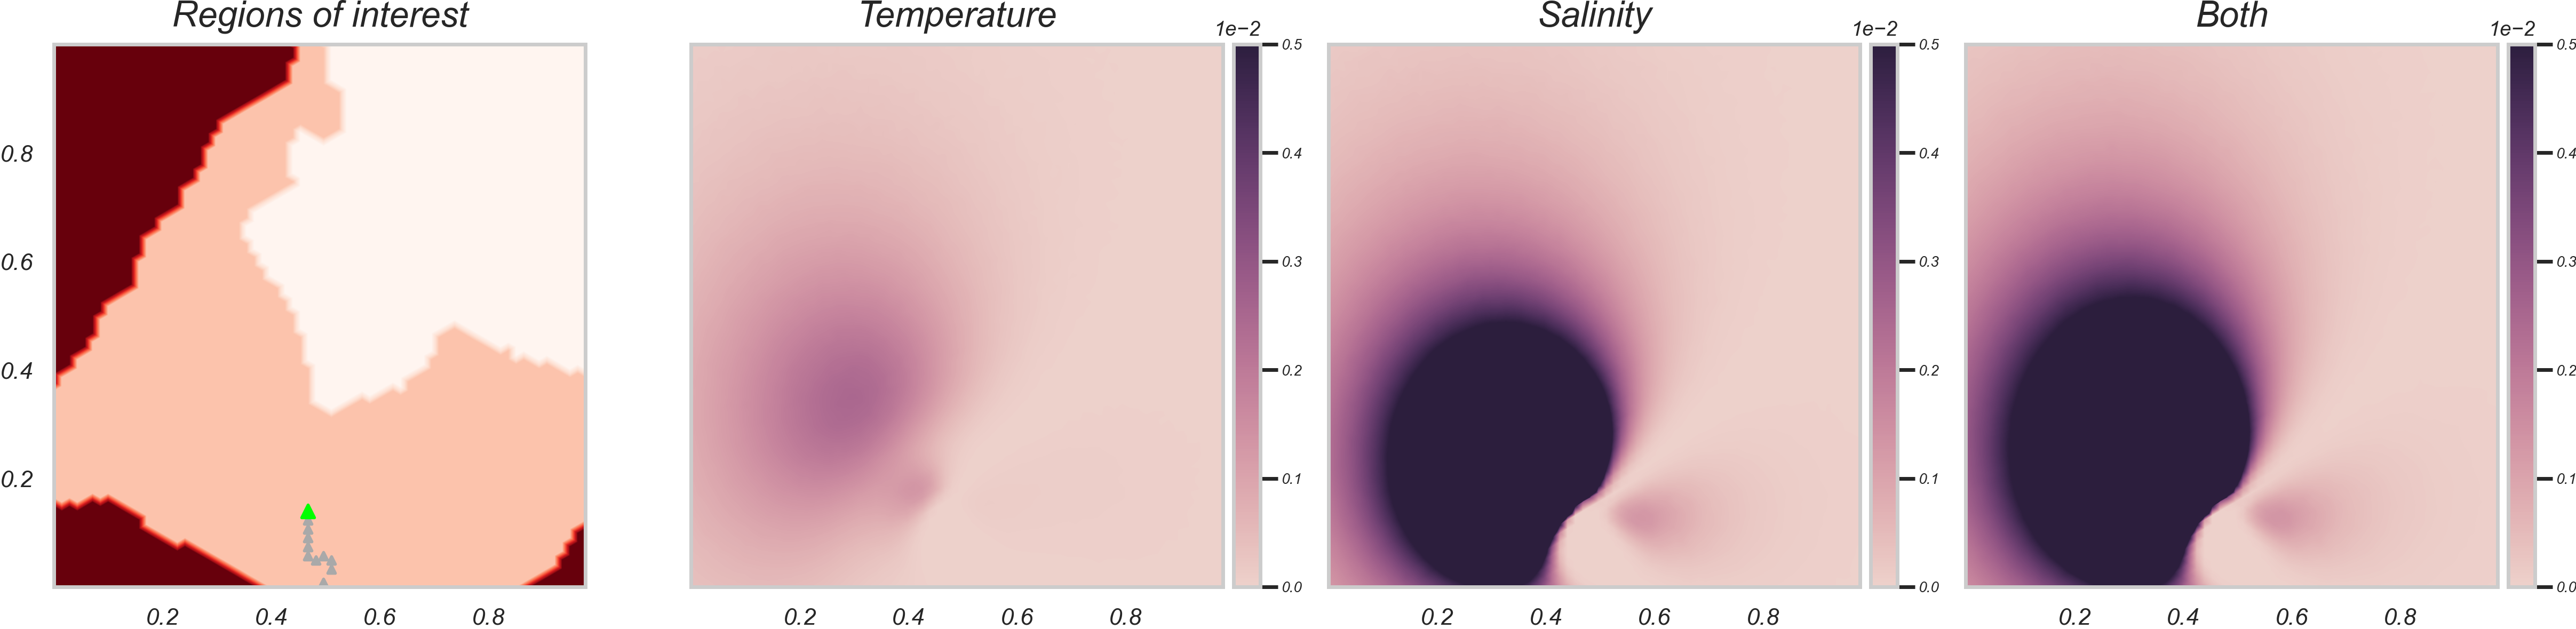
\includegraphics[width=0.99\textwidth]{Figures/ebv_comp_2.png}
  \caption{Pointwise Bernoulli variance reduction for observation of a single or both components of the random field at one location. Data collection locations in green. True excursion set in red. Places where only one response is above threshold are depicted in pink}
\label{fig:ebv_comp}
\end{figure}

Note that plotting the Bernoulli variance reduction at each point might also be used to compare different data collection plans. For example, Fig. \ref{fig:ebv_north_vs_east} shows the expected Bernoulli variance reduction associated to a data collection plan along a straight upwards line (static north) and the one associated to a straight horizontal line (static east). Both expectations are computed according to the a priori distribution of the GRF (i.e. no observations have been included yet).

\begin{figure}[h!] \centering
  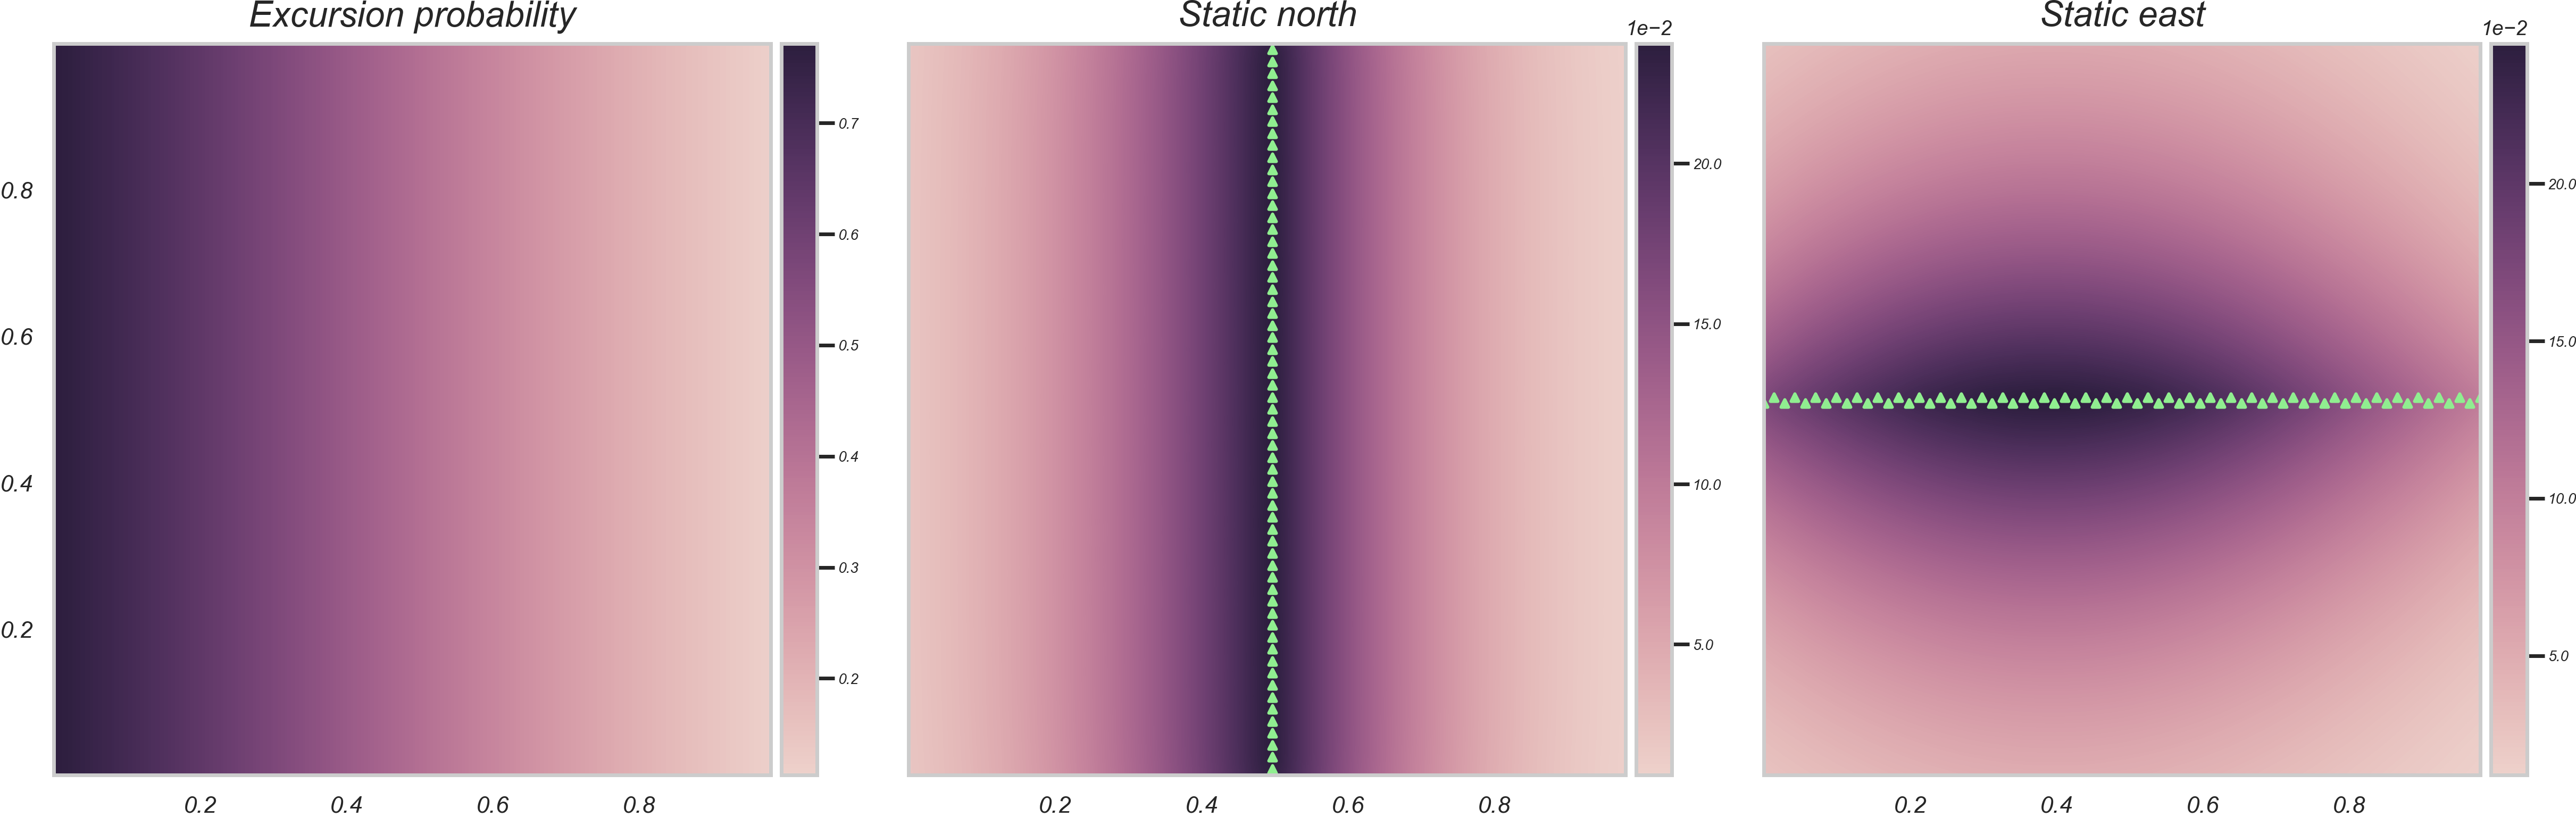
\includegraphics[width=0.99\textwidth]{Figures/ebv_north_vs_east_2.png}
  \caption{Pointwise Bernoulli variance reduction for two different observation plans. Data collection locations in green. True excursion set is in red. Places where only one response is above threshold are depicted in pink.}
\label{fig:ebv_north_vs_east}
\end{figure}

\begin{remark}
In all the above examples, the spatial domain $\domain$ has been discretized to a set of $n$ grid
locations $\mathcal{M}_g = \{\x_i, i=1,\ldots,n \}$, where each cell
has area $\Delta$; the same grid is used for the waypoint graph for
possible design locations. The EIBV is approximated by sums over all
grid cells.
\end{remark}




\section{Sequential designs and heuristic path planning}\label{sec:heuristics}

The goal of this section is to present data collection strategies that aim at decreasing the uncertainty on the target excursion set $\es$.

\subsection{Background}
As before, let $\gp$ be a $\no$-variate random field on $\domain$. See Section \ref{sec:bg_and_notation} for a recap of the specific notation used to handle mean and covariance function of multivariate random fields.

In a sequential setting, the point of view is that $n$ data collection steps have already been performed and one wants to choose what data to collect next. After each step, the GRF model is updated using the cokriging equations \ref{eq:cokrig_mean} and \ref{eq:cokrig_cov} and we will denote by $\mathbb{P}_n$ the law of the field conditional on the data gathered up to (and including) stage $n$. More generally, we will use subscripts to denote quantities conditional on the data available up to stage $\stage$. Hence, $\mu_{\stage}(\cdot)$ and $k_{\stage}(\cdot, \cdot)$ will denote conditional mean and covariance functions conditional on the first $\stage$ data collection stages.

\begin{remark}
The type of data collected at each stage can be of any type (observation of all components of the field at a single location, observation of some components only but at several locations, ...) since the concept of \textit{generalized location} allows the cokriging equations to handle all those case by putting them on equal footage.
\end{remark}

Our goal is then to optimally select what observations to do next, where the meaning of optimal is yet to be defined. Note that here again, the concept of \textit{generalized location} allows one to consider settings where only one component of the field can be observed at each step and the strategy has to choose the spatial location as well as the component to observe (heterotopic case), or settings where several observations are allowed at each stage (batch case).

We will here restrict ourselves to the case where only one spatial location can be chosen at each stage and all components of the field are observed there (isotopic case), leaving the general case for future work.


\subsection{Optimal Sequential Design}
\label{Optdes}

\textcolor{red}{(C.T.) I suspect we need this paragraph so we cite people who have to be cited. How do we want to blend it with the rest? Personally I would get rid of this subsection.}
The mathematical expression for the optimal design involves a series
of intermixed maximizations over designs and integrals over data. In
practice, the optimal solution is intractable because of the enormous
growth over stages (see e.g. \cite{sucar2015probabilistic} and
\cite{powell2016perspectives}).  Instead, we outline heuristic
strategies.

\textcolor{red}{Here introduce the fact that candidate points are always chosen in a set $\candidates$. Mention that we usually only allow a finite set. Mention that in the specific case of robot planning, we have a waypoint graph and we thus usually take $\candidates$ to be the set of current neighbouring nodes. Mention that yes, $\candidates$ normally depends on the current location (this is for robot, in general setting, depends on the location of the last observations), but we silently suppress this dependency for readability. Nevertheless, one should always remember that the current set of candidates depends on the current setting.}
\subsection{A Naive Sampling Strategy}
\label{naive}

A very simple heuristic for adaptive sampling is to greedily evaluate $Z$ at the location with current excursion probability closest to $\frac{1}{2}$.While extremely easy to implement, this strategy can lead to spend too many iterations in boundary regions regardless of the the possible effect of sampling at the considered point on the future conditional distribution of $Z$. Working in moderate dimension and having a relatively rough discretization such as the considered waypoint graph can be beneficial by helping not being stuck for too long in poorly informative regions, yet it is not really desirable to be tributary of properties of the domain discretization in order to guarantee a fair amount of exploration.  
% REFS? 


\subsection{Myopic Path Planning}
\label{sec:myopic}

The myopic (greedy) strategy which we present here is optimal if we
imagine taking only one more stage of measurements. This selection
strategy is based on expected uncertainty reduction, but it is a
heuristic because there is no anticipation of what the subsequent
designs might offer beyond the first stage.

Based on the currently available data the myopic strategy selects the location that leads to the biggest expected reduction in IBV:
\begin{criterion}[Myopic]
The next observation location $\spatloc_{\stage + 1}$ is chosen among the minimizers in $\candidates$ of the criterion:
\begin{equation}\label{critSEQ}
     C_{\text{myopic}}(u) = \EIBV_{\stage}\left(\spatloc\right)
\end{equation}
\end{criterion}

The expected IBV might be efficiently computed for each candidate points using Proposition \ref{propo2}. Once the best location has been selected, a stage of observation is performed there, the GP model is updated, yielding a conditional law $\mathbb{P}_{\stage + 1}$ and the process is repeated.

Even though this myopic strategy is non-anticipative, it still gives a
reasonable approach for creating designs in many
applications. Moreover, it can be implemented in a way that is not too demanding on computational power, making it well-suited for embedding on autonomous mobile survey platform (see Section \ref{sec:case_study} for an example).


\subsection{Look-ahead Trajectory Planning}\label{sec:LA}

We now extend the myopic strategy to a look-ahead strategy. We consider two stages of
measurements, and the strategy is then optimal in the sense that it accounts consistently for the expectations and minimizations in these two stages, but still without including any planning beyond those two steps.

\medskip

Say we have collected data up to stage $n$. The principle of two-steps lookahead
strategies is to select the next observation location $\spatloc_{\stage + 1}$ that would yield the biggest exepcted decrease in IBV if we were to (optimally) add one more observation after the one at $\spatloc_{\stage + 1}$. In order to formalize this concept, we need to be able to talk about the EIBV in the future (after observation $\stage + 1$ has been made). The definition \ref{def:eibv} of $\currentEIBV$ includes a subscript to stress that expectations are taken with respect the conditional law at stage $n$. We will extend this notion by writing $\currentEIBV(\cdot; u, y)$ to denote EIBV where expectations are taken conditional on the data available at $n$ an on an additional observation $y$ at $u$.

  \begin{criterion}[2-steps lookahead]
      The next observation location $\spatloc_{\stage + 1}$ is chosen among the minimizers in $\candidates$ of the criterion
      \begin{align}\label{critLA}
          C_{\text{2-steps}}(u) &= \mathbb{E}_{\stage}\left[\min_{\spatloc' \in
                  \candidates(\spatloc)} \EIBV_{\stage}\left(\spatloc' ; \spatloc,
      Y\right)\right]
      \end{align}
  where $Y$ is a random variable distributed according to the conditional
  law of $\gp_{\spatloc}$ at step $\stage$ (note it silently depends on the considered point
  $\spatloc$). Here, the dependence of the set of candidates on the current location has been made explicit for the second stage of measurements.
  \end{criterion}

\begin{remark}
In a practical setting, the first expectation might be computed by Monte
Carlo sampling of data $Y$ from its conditional
distribution. For each of these data samples, the second expectation
is solved using the closed-form expressions for EIBV provided by Proposition \ref{propo2}, now with conditioning on the first stage data already going into the mean and covariances in Eqs. \eqref{eq:cokrig_mean} and \eqref{eq:cokrig_cov}.
\end{remark}

\begin{remark}
All our results have been formulated in a noiseless setting. That is, to us an observation $y$ at $\spatloc$ is a realization of $\gp_{\spatloc$. Generalization to a noisy setting where $y$ is a realization of $\gp_{\spatloc} + \epsilon$ with epsilon some noise process may be performed by including noise covariance matrices where necessary.
\end{remark}

\subsection{Simulation study}
\label{sec:simulations}

\susubsection{Static and Sequential Sampling Designs}
\label{sec:sampling_designs}

%Three different designs are considered as indicated in Figure \ref{fig:stat_design}. 
%\begin{figure}[h!]
%\centering
%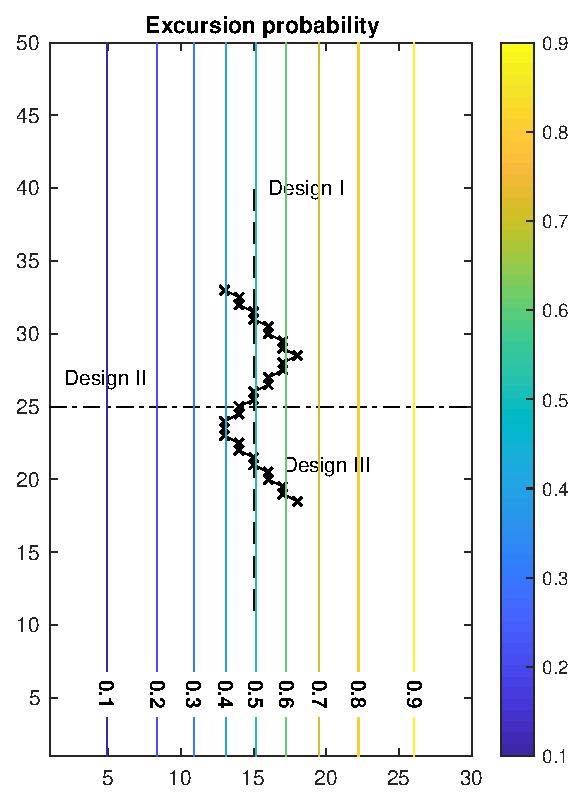
\includegraphics[width=0.65\textwidth]{Figures/Des3.eps}
%\caption{Three different static survey designs plotted on the initial EP.}\label{fig:stat_design}
%\end{figure}
%In this display the designs are plotted along with the prior probability contours of the ES for the reference parameter inputs. 

We compare three different static designs denoted
\textit{static\_north}, \textit{static\_east}, and
\textit{static\_zigzag} with the three described sequential approaches
\textit{naive}, \textit{myopic}, and \textit{look-ahead}. The static
sampling paths are pre-determined and cannot be altered and represent
the pre-planned strategies used in most current AUV operational survey
designs.

For a fixed survey length, a closed-form expression for the EIBV is
available as in Propositoin \ref{propo_eibv}
. However, for the sequential
approaches this is not the case. For comparison the properties are
therefore evaluated using Monte Carlo sampling over several replicates
of realizations from the model while conducting simulated sequential
surveys for each one. We also compare predictive
performance measured by root mean square error (RMSE) for temperature
and salinity estimates as well as also the variance reduction in these
two variables. It is important to note that the objective function
used by the agent \kc{First of 'agent'. Define it or change it
  to 'robot'? Note further uses below.} is focused on reducing the
EIBV, but we nevertheless expect that we will achieve good predictive
performance for criteria such as RMSE as well. Another non-statistical
criteria that is important for practical purposes is the computational
time needed for the strategy, as this will impact the performance for
an embedded system.

%\begin{figure}[h!]
%\centering
%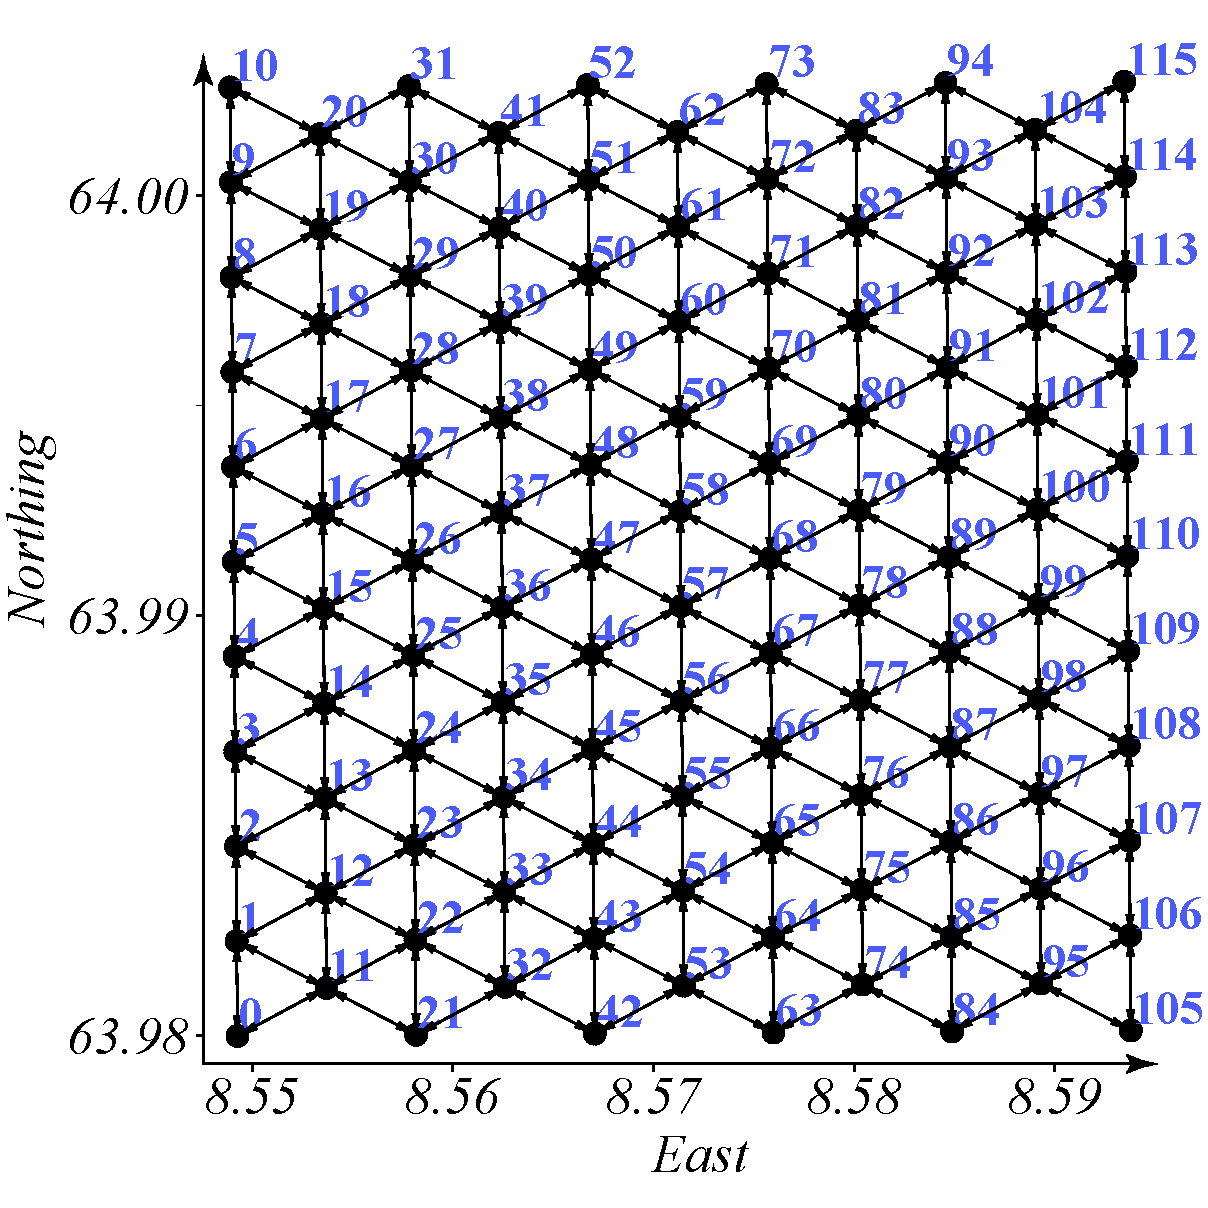
\includegraphics[width=0.50\textwidth]{Figures/sim/wp_graph_paper.pdf}
%\caption{The equilateral waypoint graph used to discretize the
%  trajectory choices over the $31\times31$ grid used to discretize the GP.}
%\label{fig:wp_graph}
%\end{figure}

\begin{figure}[!h] 
\centering 
\subfigure[The waypoint graph.]{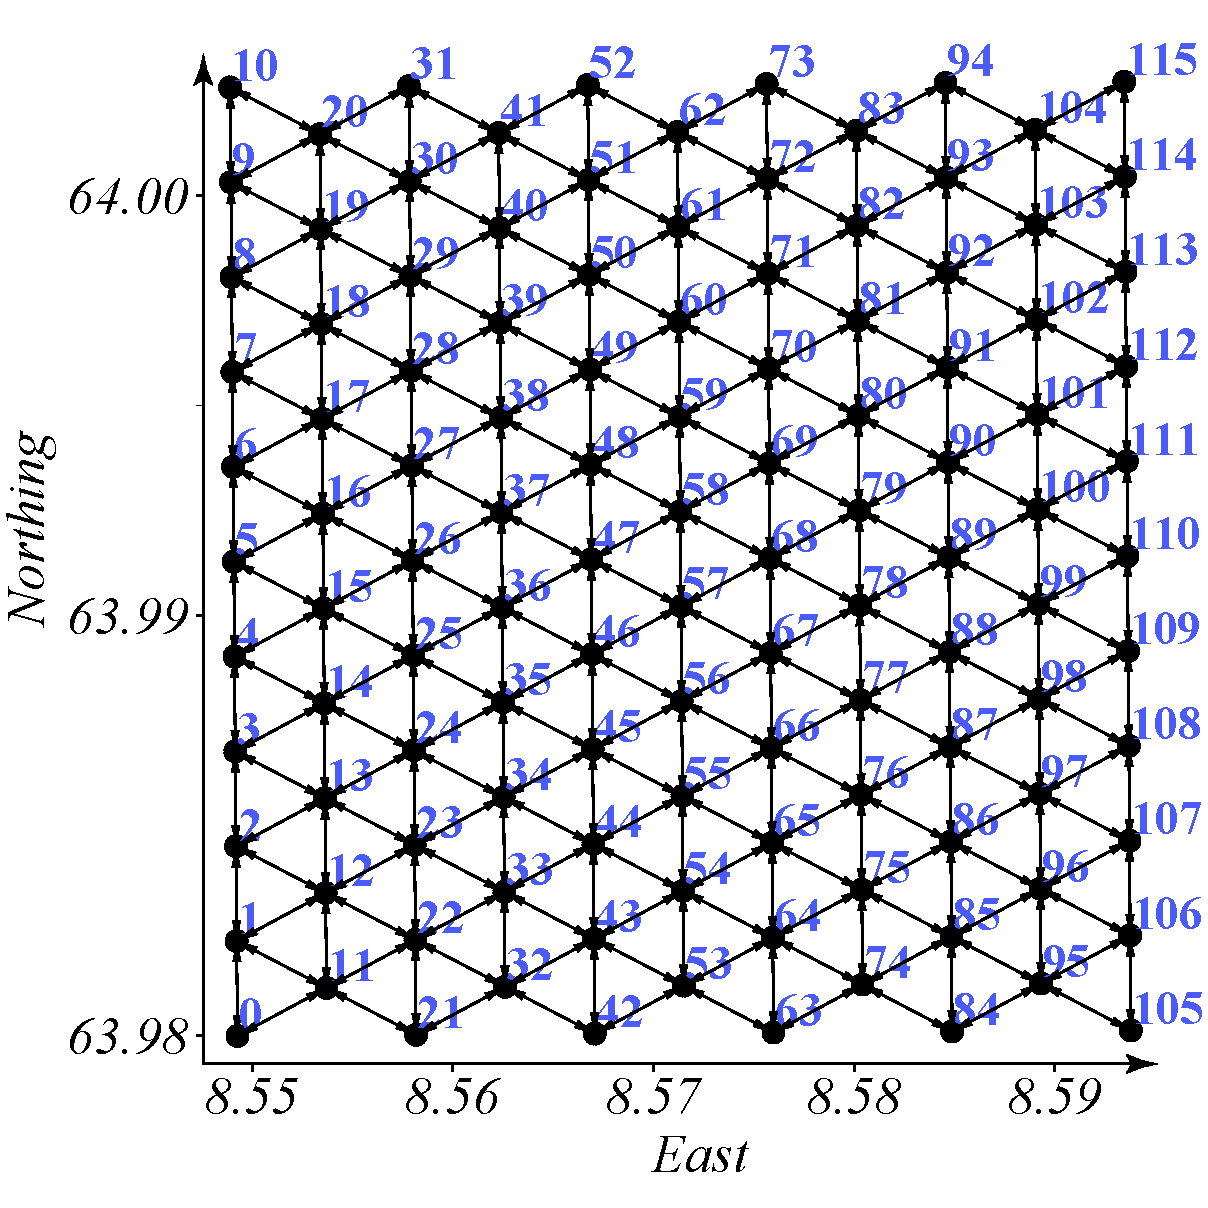
\includegraphics[width =
0.49\textwidth]{Figures/sim/wp_graph_paper.pdf}\label{fig:wp_graph_a}}
\hfill
\subfigure[The waypoint graph in 3D.]{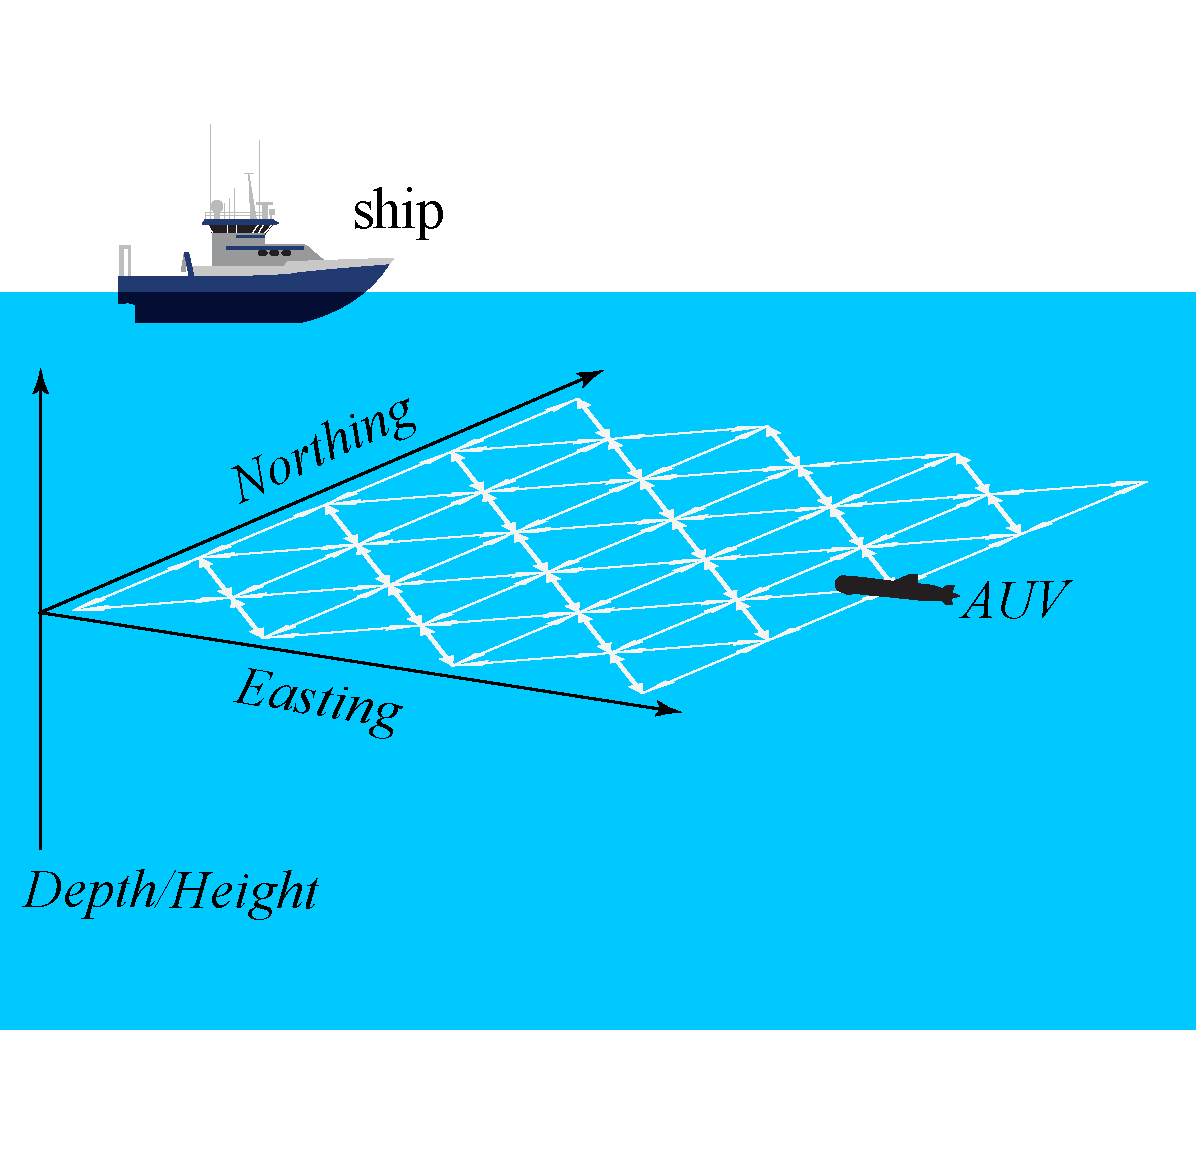
\includegraphics[width =
0.49\textwidth]{Figures/sim/wp_graph_3d.pdf}\label{fig:wp_graph_b}}
\caption{\ref{fig:wp_graph_a} The equilateral waypoint graph used to discretize the
trajectory choices over the $31\times31$ grid used to discretize the GP.
\ref{fig:wp_graph_b} The waypoint grid shown in a 3D environment.}
\label{fig:wp_graph}
\end{figure}

Each strategy is conducted on an equilateral grid as shown in
Fig. \ref{fig:wp_graph}. The sequential sampling agent starts at the
center East-West coordinate at the southern end of the domain (node 53
\kc{Maybe color this node differently and modify the caption?}). The
AUV moves along edges in the waypoint graph while the vehicle makes
measurements. The data is assimilated into the GP model before an
evaluation of the next node to sample is conducted at the end of the
edge.

\subsection{Simulation Results}

A total of 100 replicate simulations were conducted with all
strategies. The results are shown in Fig. \ref{fig:sim_results}, where
the different criteria are plotted as a function of survey
distance. Fig. \ref{fig:avg_ev} shows the resulting drop in IBV for
each of the six strategies. IBV reduction occurs most under the
\textit{myopic} and \textit{look-ahead} strategies, each performing
almost equally; this is expected as the two criteria
(Eq. \eqref{critSEQ} and \eqref{critLA}) are sensitive to differences
in IBV. The \textit{static\_north} design also does well here because
the path is parallel to the boundary between the water masses.

\begin{figure}[h!]
  \centering
  % \subfigure[Excursion set variance $E_{\by}(p[1-p])$.]{\label{fig:avg_ev}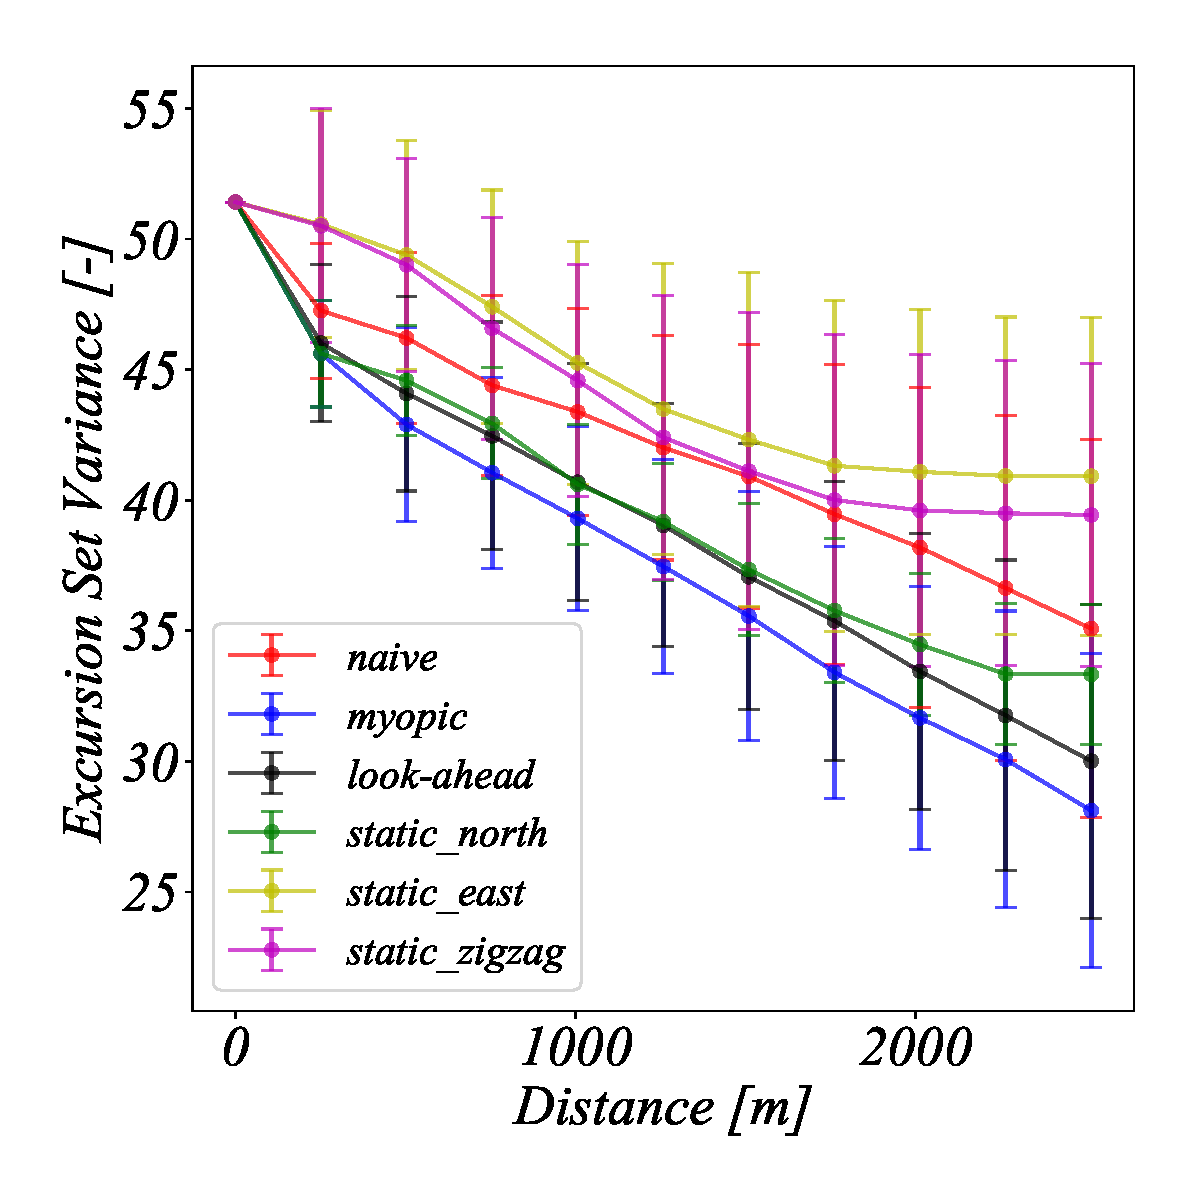
\includegraphics[height=0.49\textwidth]{Figures/sim/avg_EV.pdf}}
  \subfigure[IBV.]{\label{fig:avg_ev}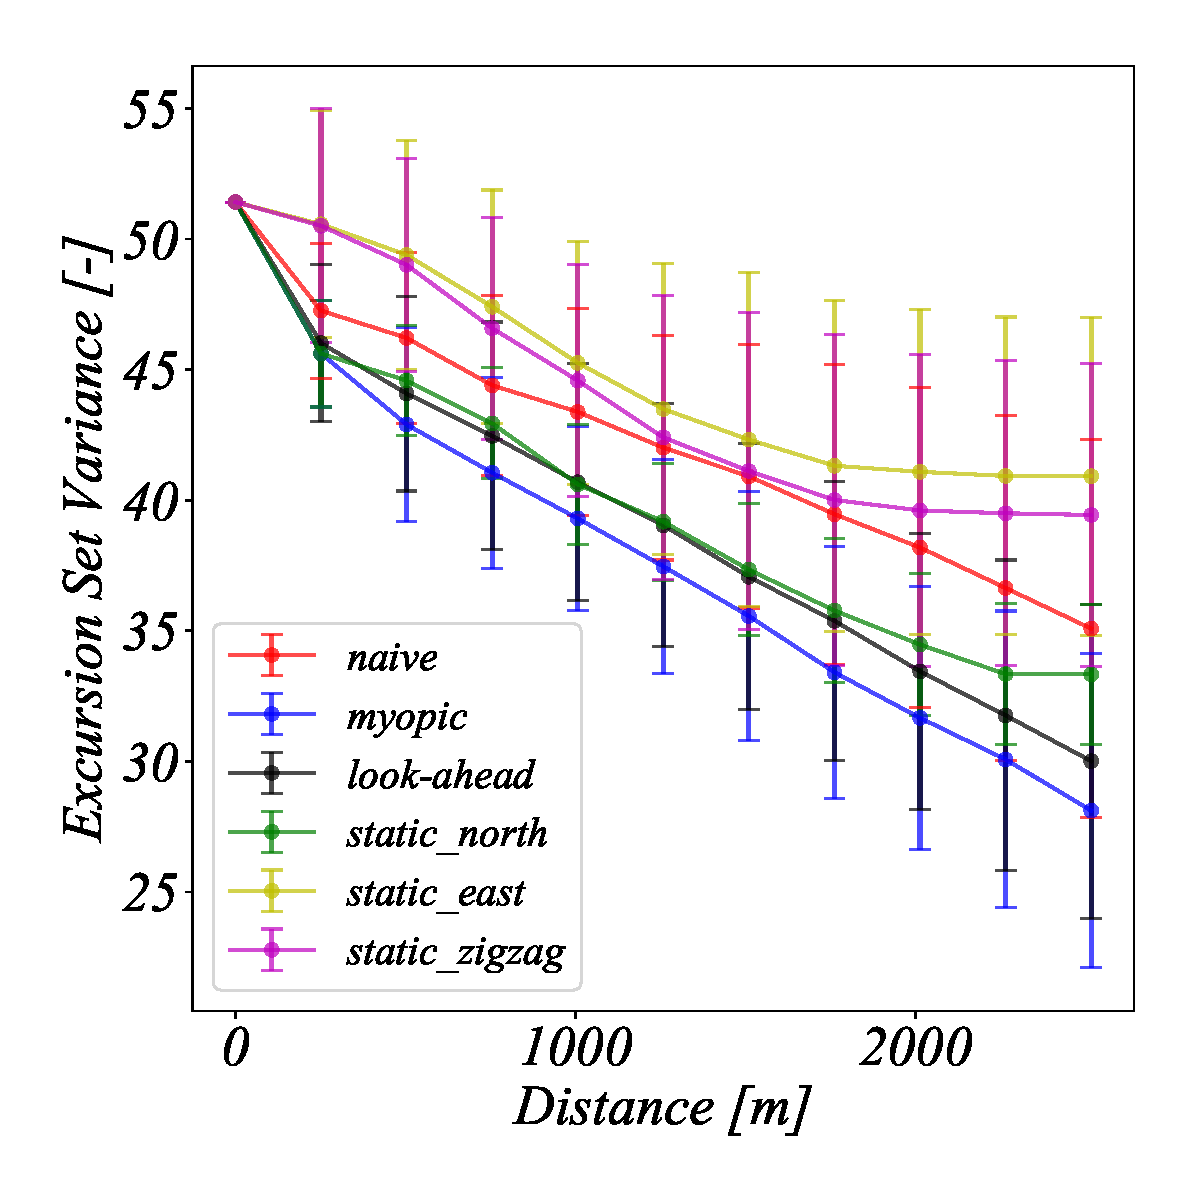
\includegraphics[height=0.49\textwidth]{Figures/sim/avg_EV.pdf}}
  \hfill
  \subfigure[RMSE between estimated field and truth.]{\label{fig:avg_rmse}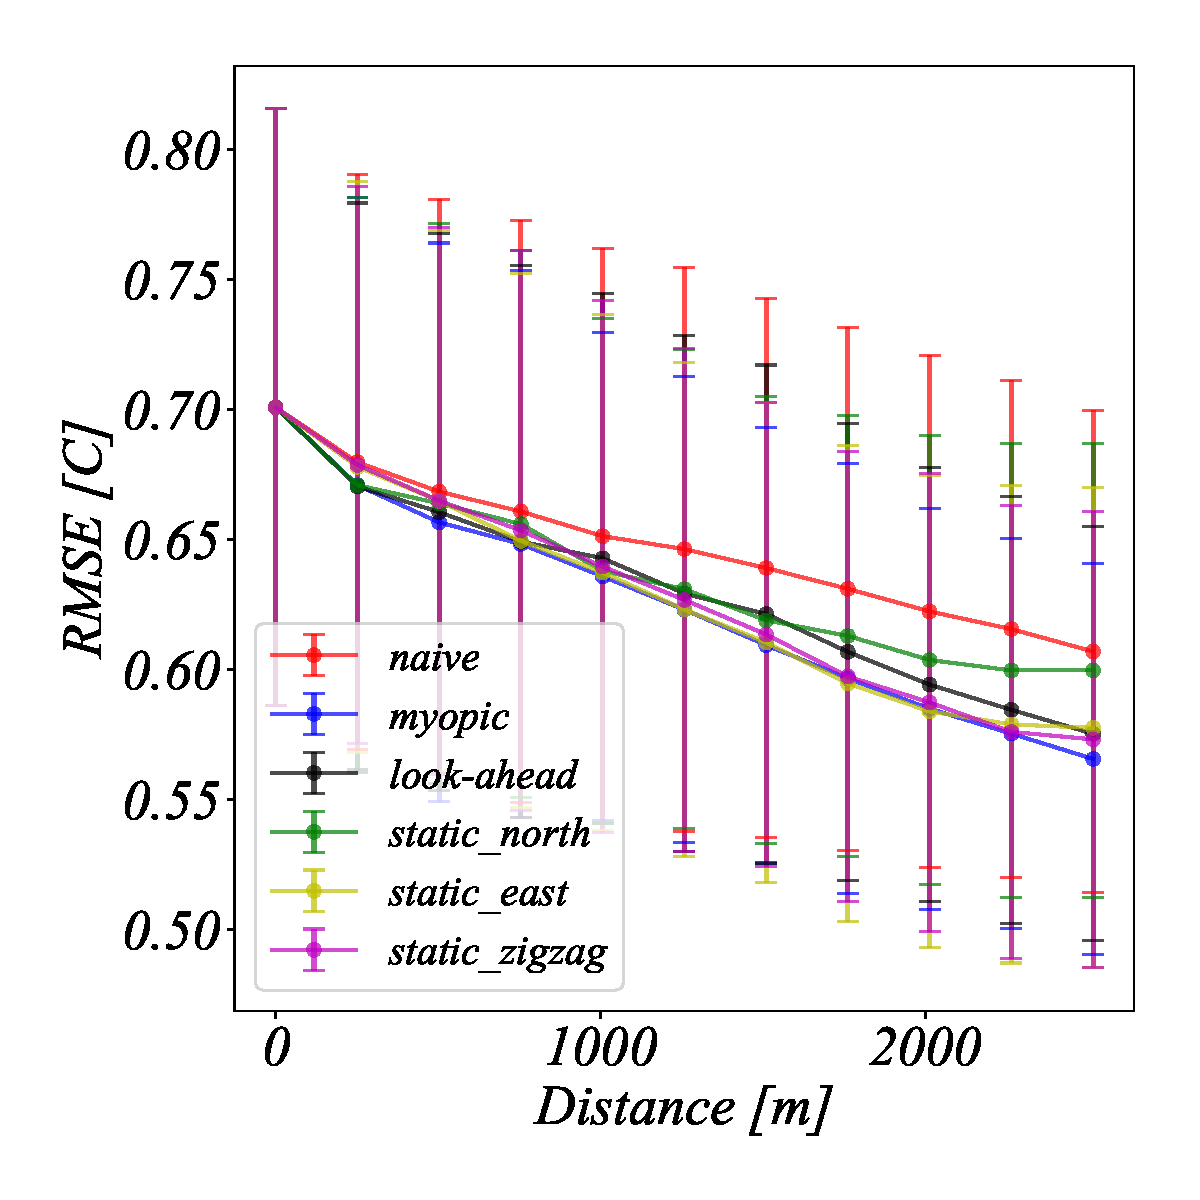
\includegraphics[height=0.49\textwidth]{Figures/sim/avg_RMSE.pdf}}
  \hfill 
  \subfigure[Explained variance $\bR^{2}$.]{\label{fig:avg_r2}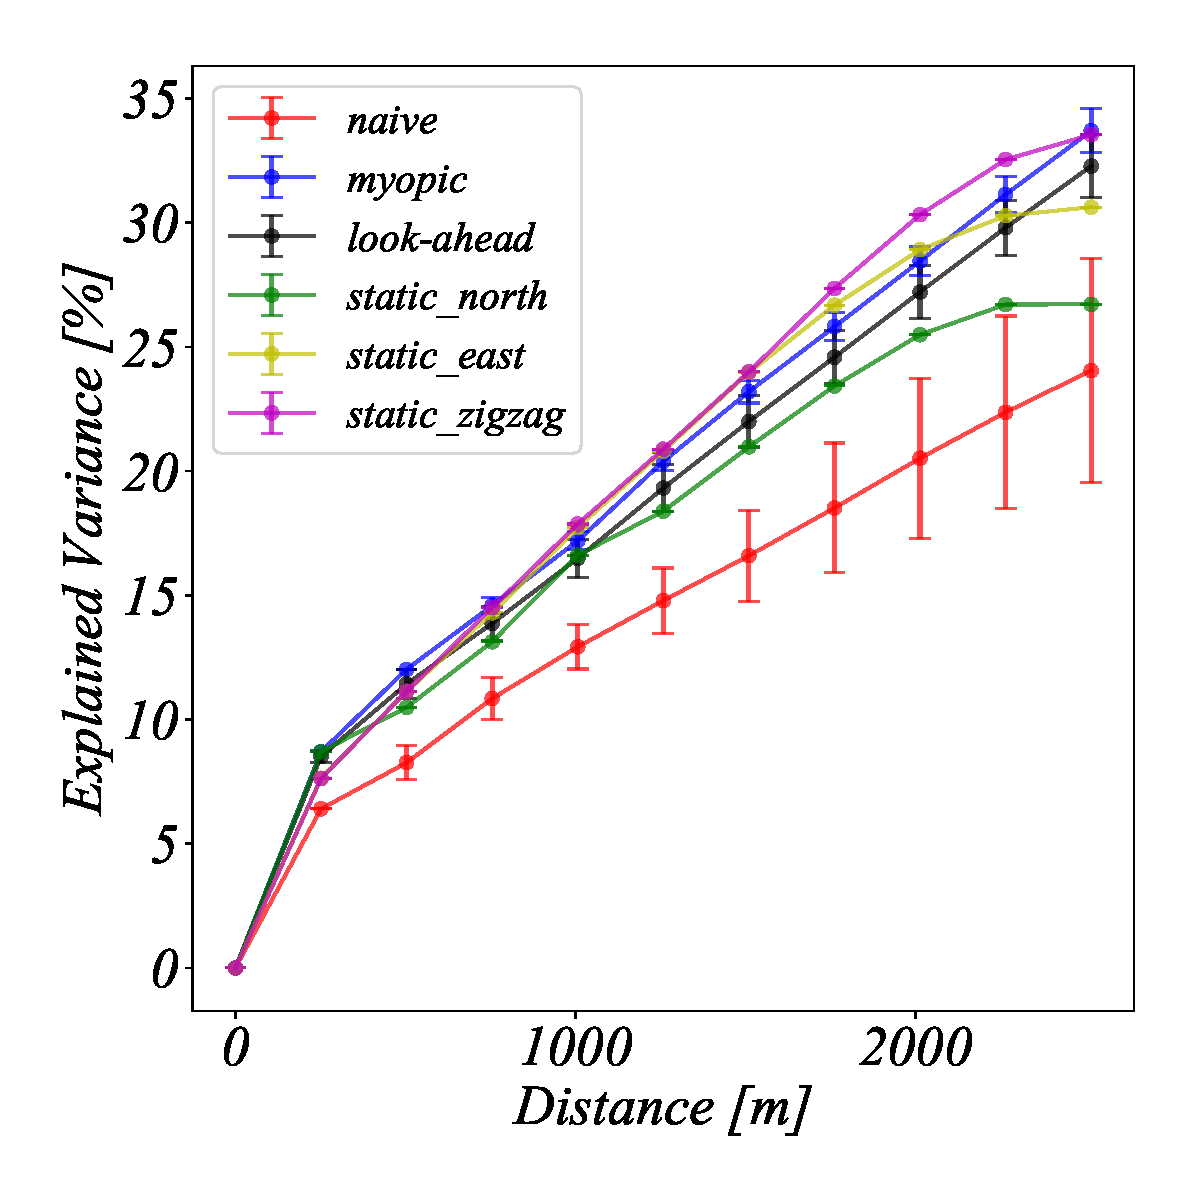
\includegraphics[height=0.49\textwidth]{Figures/sim/avg_R2.pdf}}
  \hfill 
  \subfigure[Computational time for inferencing.\kc{I see only 
    lines associated with 4 variables showing in the graph. Where is
    static\_north and static\_east?}]{\label{fig:avg_time}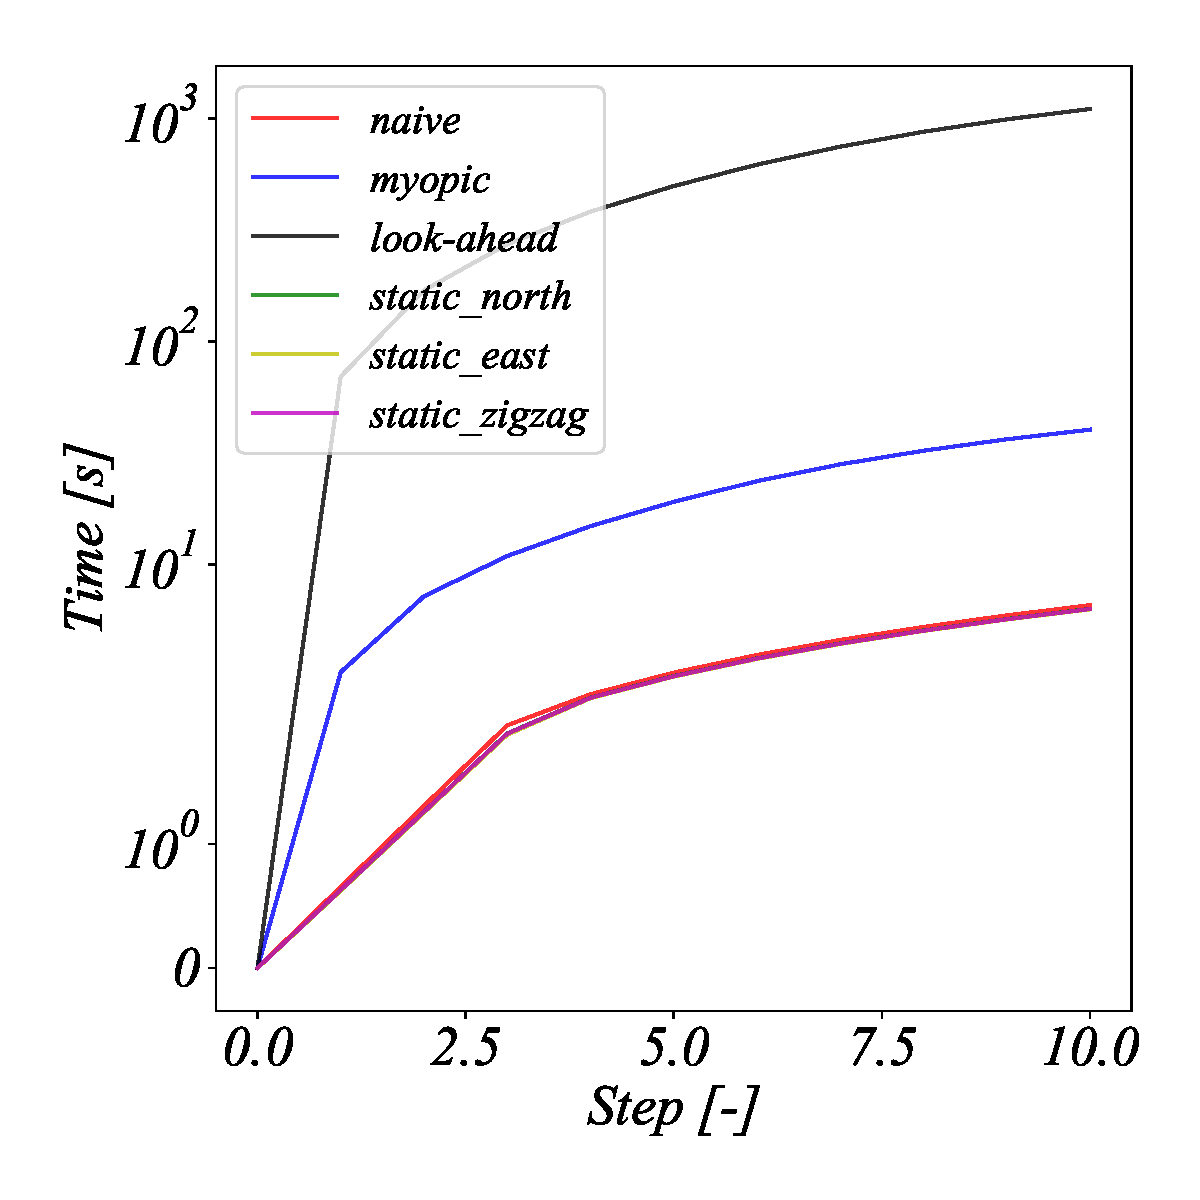
\includegraphics[height=0.49\textwidth]{Figures/sim/avg_Time.pdf}} 
\caption{Simulation results from 100 replicate simulations for 10
  sampling choices/stages on the grid. \kc{Vertical lines show large
    variation in replicate results.}}  
\label{fig:sim_results}
\end{figure}

Fig. \ref{fig:avg_rmse} and \ref{fig:avg_r2} show the resulting drop
in RMSE and increase in explained variance, respectively. Both
\textit{myopic} and \textit{look-ahead} strategies perform well here,
but some of the \textit{static\_east} and \textit{static\_zigzag} also
achieve good results because they are pre-determined to cover large
parts of the domain without re-visitation. Sequential strategies
targeting IBV will sometimes not reach similar coverage, as
interesting data may draw the path into twists and turns. There is
relatively large variety in the replicate results as indicated by the
vertical lines. Nevertheless, the ordering of strategies is similar.


Fig. \ref{fig:avg_time} shows the computational effort: the
\textit{naive} strategy is on par with the static designs, while the
\textit{myopic} strategy is slower. The \textit{look-ahead} is even
slower, reaching levels that are nearly impractical for execution on a
vehicle. Some pruning of the graph is performed to improve the
performance, such as ruling out repeated visitations and
back-and-forth routes. Some of the intermediate results are also
stored for longer planning horizons. Further pruning of branches or
inclusion of other heuristics could be included for better
performance. Then again, the inclusion of heuristics is likely a
contributing factor for the \textit{look-ahead} strategy failing to
outperform the \textit{myopic} strategy.

In Fig. \ref{fig:route_choices}, the realized sampling paths for each
of the sequential schemes and static designs are shown. The
\textit{naive} strategy often gets stuck in the southern part of the
domain because it is too focused on the probabilities near $0.5$. The
\textit{myopic} strategy covers a wider domain than the naive or
look-ahead. There are several reasons for this. First, a greedy
approach will tend to put more emphasis on promising locations close
to the agent, which may lead away from the centre. Second, as the
agent evaluates the impact of locations further away (look-ahead)
where assimilated data has less predictive power, the GP model (which
is centered here) will act to restrict paths deviating from the
central zone.

We studied the sensitivity of the results by modifying the input
parameters to have different correlations between temperature and
salinity, standard deviations, and spatial correlation range.  In all
runs, the \textit{myopic} and \textit{look-ahead} strategies perform
the best in terms of realized IBV, and much better than
\textit{naive}. The \textit{look-ahead} strategy seems to be
substantially better than the \textit{myopic} design only for very
small initial standard deviation or very large spatial correlation
range. \textit{static\_north} continues to be the best static design
for IBV, while \textit{static\_zigzag} is the best design for the
other predictive performance measures, especially so with large
spatial correlation range. We also ran simulation studies with only
temperature data, and for realistic correlation levels between
temperature and salinity, the IBV results are not much worse when only
temperature data are available. In addition to the comparison made in
Table \ref{tab:sim_rhoab}, the current setting includes spatial
correlation and this likely reduces the additional influence of having
bivariate data. However, it seems that having temperature data alone
does a substantially worse job in terms of explained variance































\section{Case Study - Mapping a River Plume}
\label{sec:case_study}

To demonstrate the applicability of using multivariate EPs and the IBV
to inform oceanographic sampling, we present a case study mapping a
river plume with an AUV. The experiment was performed in Trondheim,
Norway, surveying the Nidelva river (Fig. \ref{fig:nidelven}). The
experiments were conducted in late Spring 2019, when there is still
snow melting in the surrounding mountains so that the river water is
substantially colder than the water in the fjord. The experiment was
focused along the frontal zone that runs more or less parallel to the
eastern shore as noted in Fig. \ref{fig:nidelven}.

\subsection{Model Specification}
\label{sec:exp_modeling}

The statistical model parameters were specified based on a short
preliminary survey where the AUV made an initial transect to determine
the trends in environmental conditions and correlation
structures. Based on the initial data, the trend parameters were
estimated by linear regression, where both temperature and salinity
are assumed to increase linearly, going west from the river
mouth. Next, the residuals from the regression analysis were analyzed
to study the fit of the GP model and to specify the covariance
parameters.

%\begin{figure}[!h] 
% \centering 
%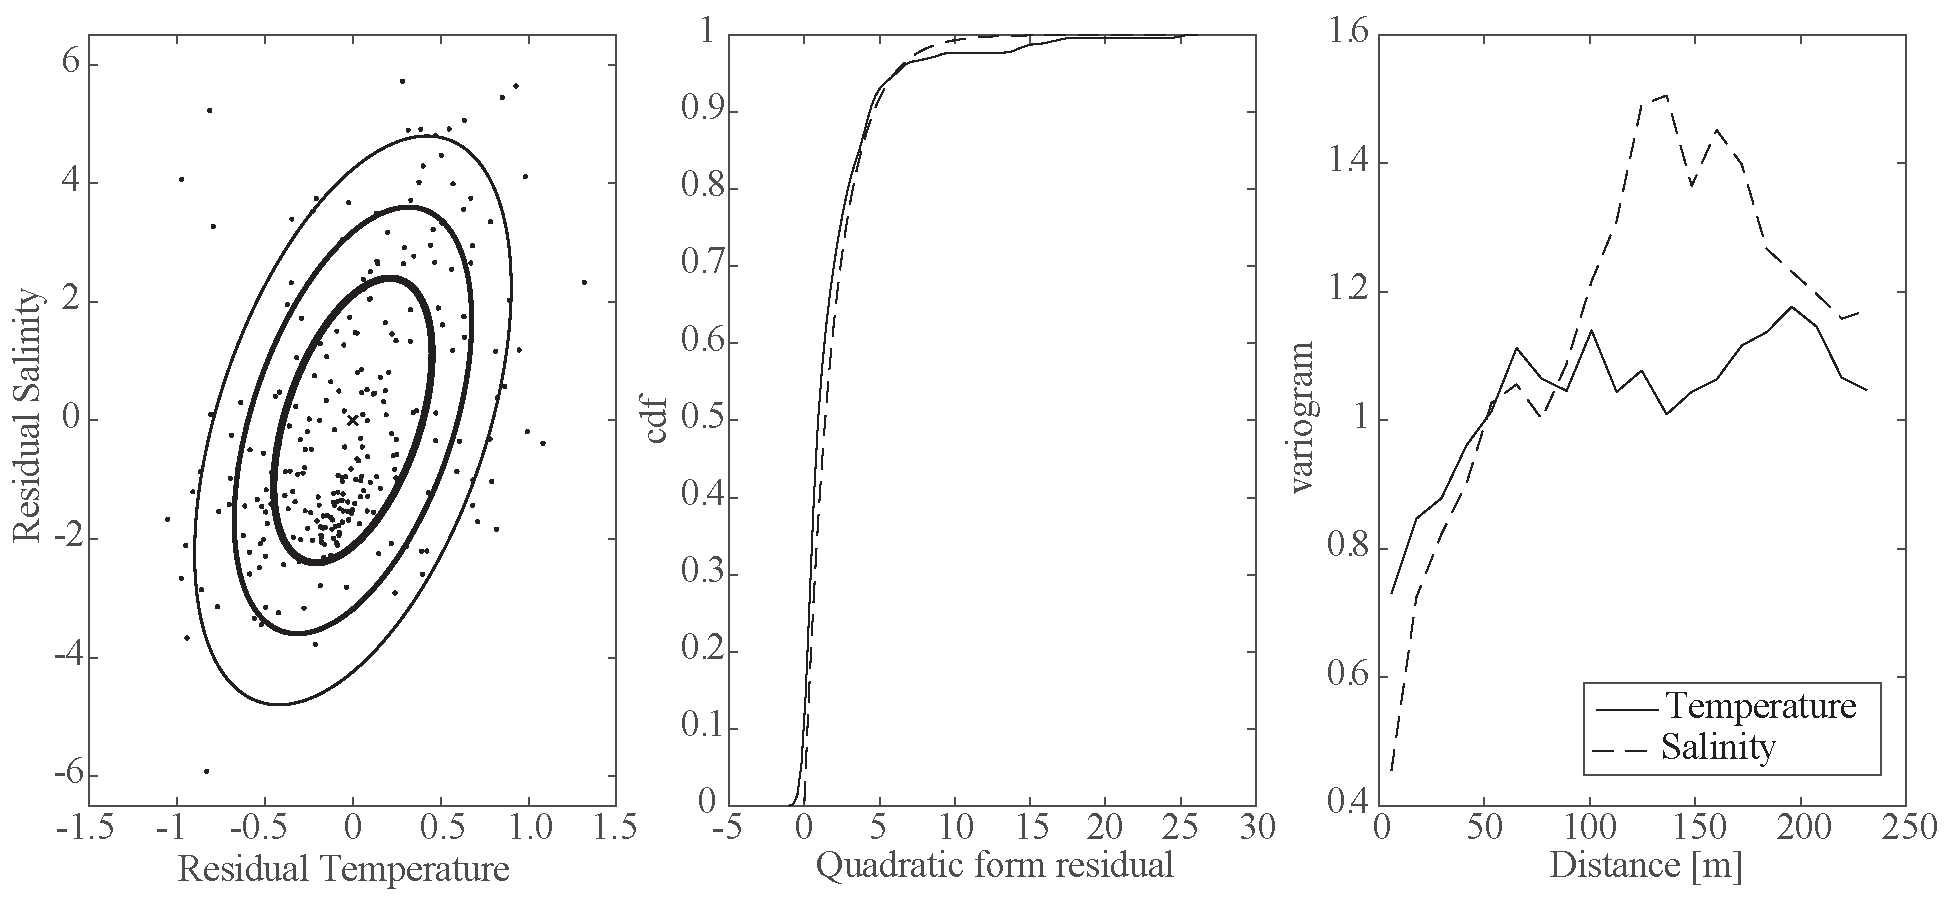
\includegraphics[width=0.98\textwidth]{Figures/field-trials/res_diag.pdf}
%\caption{Data analysis from a preliminary trial experiment using the
%  AUV. Left: Residual plot of temperature and salinity along with
%  Gaussian contours. Middle: Empirical CDF (solid) of the quadratic form of
%  the residuals along with the theoretical CDF (dashed) of the $\chi^2$
%  distribution with two degrees of freedom. Right: Empirical variogram
%  of the salinity and temperature data.} \label{fig:parest}
%\end{figure}

\begin{figure}[!h]
  \centering
  \subfigure[Residual plot.]{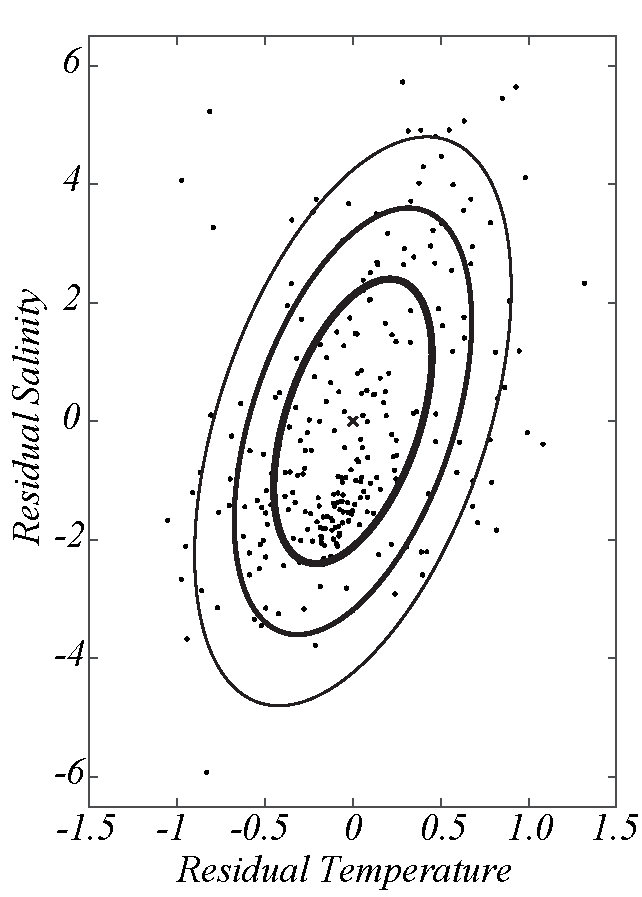
\includegraphics[width = 0.32\textwidth]{Figures/field-trials/res_diag_a.pdf}\label{fig:parest_a}}
  \hfill
  \subfigure[Empirical CDF.]{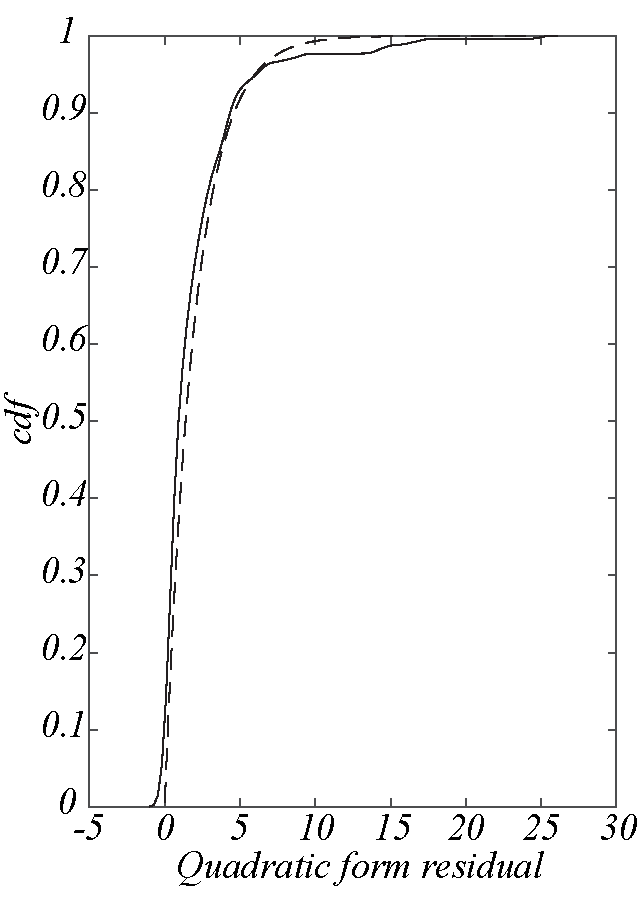
\includegraphics[width = 0.32\textwidth]{Figures/field-trials/res_diag_b.pdf}\label{fig:parest_b}}
  \hfill
  \subfigure[Empirical variogram.]{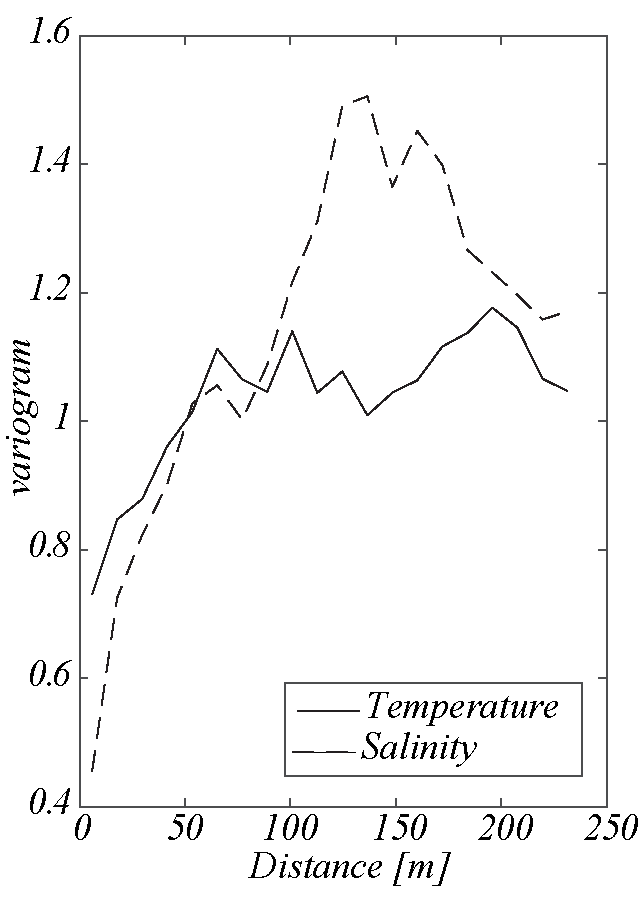
\includegraphics[width = 0.32\textwidth]{Figures/field-trials/res_diag_c.pdf}\label{fig:parest_c}}
  \caption{Data analysis from a preliminary trial experiment using the
    AUV. \ref{fig:parest_a} Residual plot of temperature and salinity
    along with Gaussian contours. \ref{fig:parest_b} Empirical CDF
    (solid) of the quadratic form of the residuals along with the
    theoretical CDF (dashed) of the $\chi^2$ distribution with two
    degrees of freedom. \ref{fig:parest_c} Empirical variogram of the
    salinity and temperature data.}
\label{fig:parest}
\end{figure}

Fig. \ref{fig:parest} summarizes diagnostic plots of this
analysis. Fig. \ref{fig:parest_a} shows a cross-plot of temperature
and salinity residuals after the westerly trends in both salinity and
temperature are subtracted from the data. This scatter-plot of joint
residuals indicates larger variability in salinity than in
temperature, and a positive correlation ($0.5$) between the two
variables. Based on the fitted bivariate Gaussian model (ellipses in
Fig. \ref{fig:parest_a}), we can compute the modeled quadratic form of
the residuals, and if the model is adequate they should be
approximately $\chi^2_2$ distributed. Fig. \ref{fig:parest_b} shows
the empirical cumulative distribution function (CDF) of these
quadratic forms (solid) together with the theoretical CDF of the
$\chi^2_2$ distribution. The modeled and theoretical curves are very
similar, which indicates that the Gaussian model fits reasonably
well. Even though there appears to be some clustering in both
Fig. \ref{fig:parest_a} and \ref{fig:parest_b}, the bivariate
diagnostic plots look reasonable and justify a Gaussian
model. Fig. \ref{fig:parest_c} shows the empirical variogram of the
scaled residuals for temperature and salinity. The decay is similar
for the two, and seems to be negligible after about $150$ m.


Based on the analysis in Fig. \ref{fig:parest}, the resulting
parameters are given in Table \ref{tab:experiment_param}. The
regression parameters shown here are scaled to represent the east and
west boundaries of the domain as seen in the preliminary transect
data, and the thresholds are intermediate values. These parameter
values were then used in field trials where we explored the
algorithm's ability to characterize the river plume front separating
the river and fjord water masses, providing a spatial map of this
boundary.

%Mapping the spatial extent of a frontal zones is an important problem for studying many bio-physical interactions in the ocean. The frontal zone is determined by the boundary where plumes of sediments, nutrients, and possibly pollutants spreading from the river outlet meet and interact with adjacent coastal water. Due to the lower density the plumes spread on the surface, creating a front with an sharp gradient in both temperature and salinity. 

\begin{table}[!h]
\centering
\begin{tabular}{lrr}
\toprule
Parameter & Value & Source\\
\midrule
\rowcolor{Gray}
Cross correlation temp. and sal. & 0.5 & AUV observations\\
Temp. variance &  0.20 & AUV observations (variogram)\\
\rowcolor{Gray}
Sal. variance &  5.76 & AUV observations (variogram)\\
Corr. range  & 0.15 km & AUV observations (variogram)\\
\rowcolor{Gray}
River temp. $T_{river}$ & $10.0\,^{\circ}\mathrm{C}$ & AUV observations\\
Ocean temp. $T_{ocean}$ & $11.0\,^{\circ}\mathrm{C}$ & AUV observations\\
\rowcolor{Gray}
River sal. $S_{river}$ & $14.0$ g/kg & AUV observations\\
Ocean sal. $S_{ocean}$ & $22.0$ g/kg & AUV observations\\
\rowcolor{Gray}
Threshold temp. & $10.5\,^{\circ}\mathrm{C}$ & $(T_{ocean}-T_{river})/2+T_{river}$\\
Threshold sal. & $18.0$ g/kg & $(S_{ocean}-S_{river})/2+S_{river}$\\
\rowcolor{Gray}
\bottomrule
\end{tabular}
\caption{Model and threshold parameters from an initial AUV
  survey. Observations were taken across the front while crossing from
  fresh, cold river water to saline and warmer ocean waters. \kc{Might
  be good to expand the terms and not have abbreviations in the table
  above; there's plenty of space.}}
\label{tab:experiment_param}
\end{table}


\subsection{Experimental Setup}

The sampling locations were distributed over an equilateral grid, as
shown in the grey-colored lattice in Fig. \ref{fig:map}. The robotic
platform consisted of a Light AUV \citep{sousa2012lauv}
(Fig. \ref{fig:lauv}) equipped with a 16 Hz Seabird Fastcat-49
conductivity, temperature, and depth (CTD) sensor providing
temperature and salinity
measurements. %The accuracy of the CTD instrument is $\pm 0.0003$ S/m (conductivity) and $\pm0.002\,^{\circ}\mathrm{C}$ (temperature).
The sampling agent was built on top of the autonomous agent framework
Teleo-Reactive EXecutive (\textit{T-REX})
\citep{py10,Rajan12,Rajan12b}, running an instance of the
\textit{myopic} strategy from Section \ref{sec:myopic} to 
control the
AUV and decide between sampling locations.

\textcolor{blue}{TO BE MERGED WITH THE PARA ABOVE? The AUVs considered here are powered untethered platforms, that
operate at $1$-$3$ m/s in the upper water column, where they are free
to move in six degrees of freedom (6 DOF). The in-water operation time
capability depends on survey speed, payload sensors and navigation;
typically this amounts to 8-48 hrs. AUVs typically use single-board
computers (SBCs), like the Raspberry Pi or a multicore GPU NVIDIA
Jetson TX1 (quad-core 1.91 GHz 64-bit ARM machine, a 2-MB L2 shared
cache, and 4 GB of 1600 MHz DRAM) for computation onboard.}

\begin{figure}[!h] 
\centering 

\includegraphics[width=0.98\textwidth]{Figures/harald.jpg}
\caption{The commercially available Light Autonomous Underwater
  Vehicle (LAUV) platform for upper water-column exploration used in
  our experiments.}
\label{fig:lauv}
\end{figure} 

The sampling strategy was designed around the concept of visiting
waypoints sequentially. Arriving at a desired waypoint with new
measurements and an updated model, the AUV triggers the myopic
strategy to evaluate the different design criteria (see
Eq. \eqref{critSEQ}). The waypoint-and-path combination that is
expected to reduce the IBV the most is selected, and upon arrival this
procedure is then repeated. At each stage, it takes the AUV about 30
seconds to evaluate the EIBV for all the possible waypoint-and-path
alternatives.

The AUV was set to start in the south-center part of the waypoint
graph, with the previously outlined GP model of the environment
(Section \ref{sec:exp_modeling}). A survey was set to take
approximately 40 minutes, visiting 15 waypoints on the grid, with the
AUV running near the surface to capture the plume. On its path from
one waypoint to the next, the AUV gathered data regularly, and the GP
model assimilated temperature and salinity data with an update
frequency of 30 seconds, giving about three updates per stage.

\begin{figure*}[!h]
\centering
\subfigure[AUV survey area]{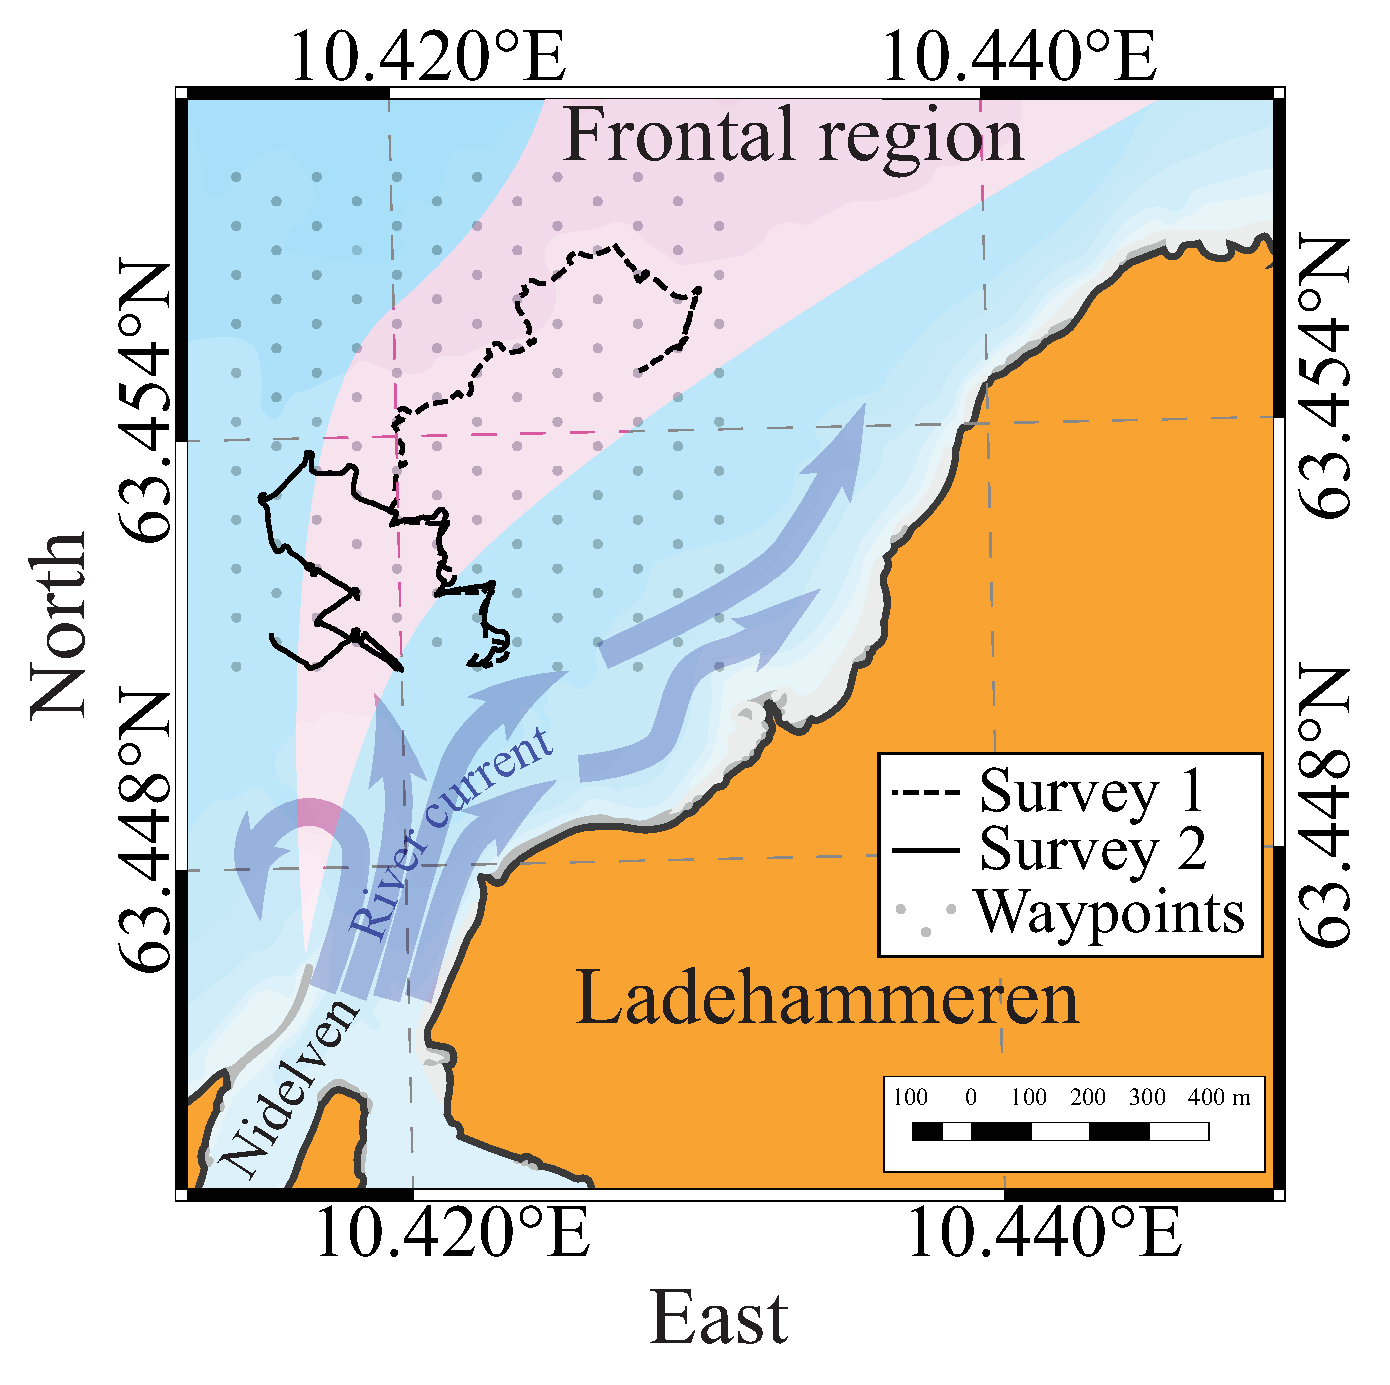
\includegraphics[height=0.41\textwidth]{Figures/field-trials/alt_map.eps}\label{fig:map}}
\hspace{0.3cm}
\subfigure[Temperature tracks]{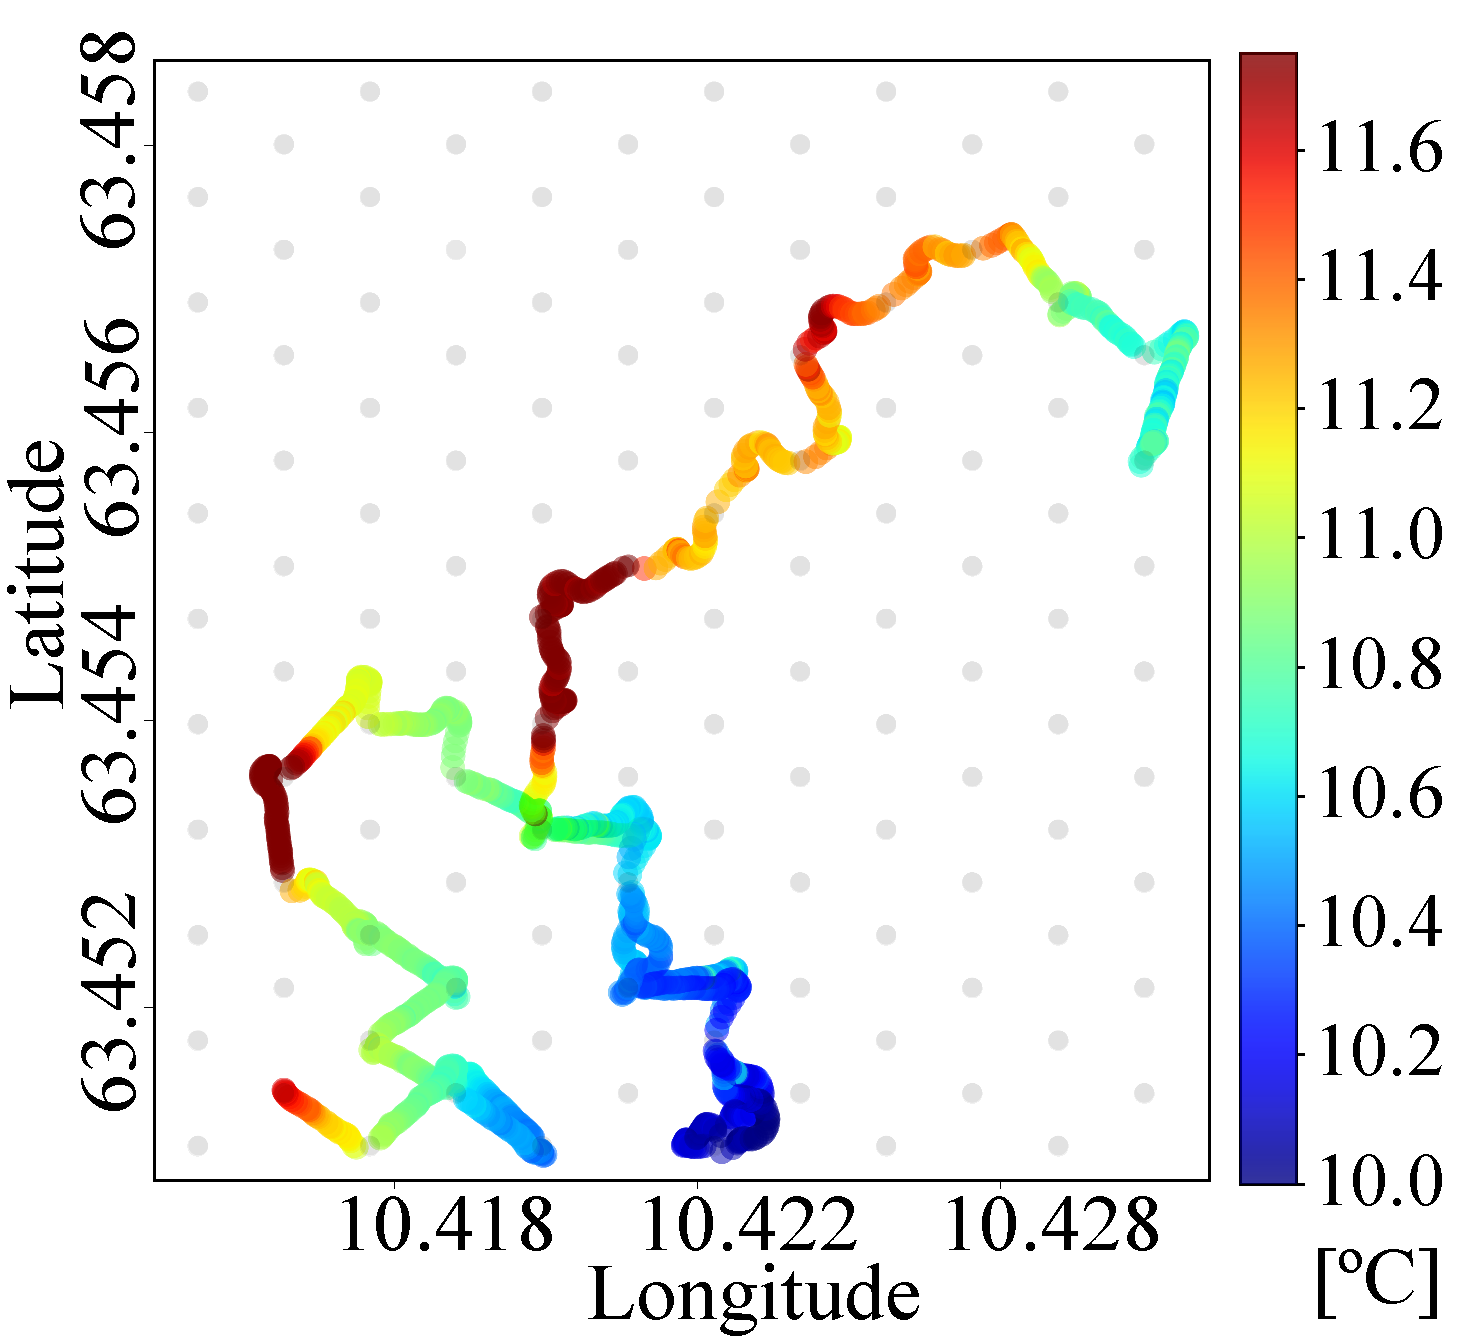
\includegraphics[height=0.41\textwidth]{Figures/field-trials/auv.pdf}\label{fig:res_both}}

\subfigure[Survey 1]{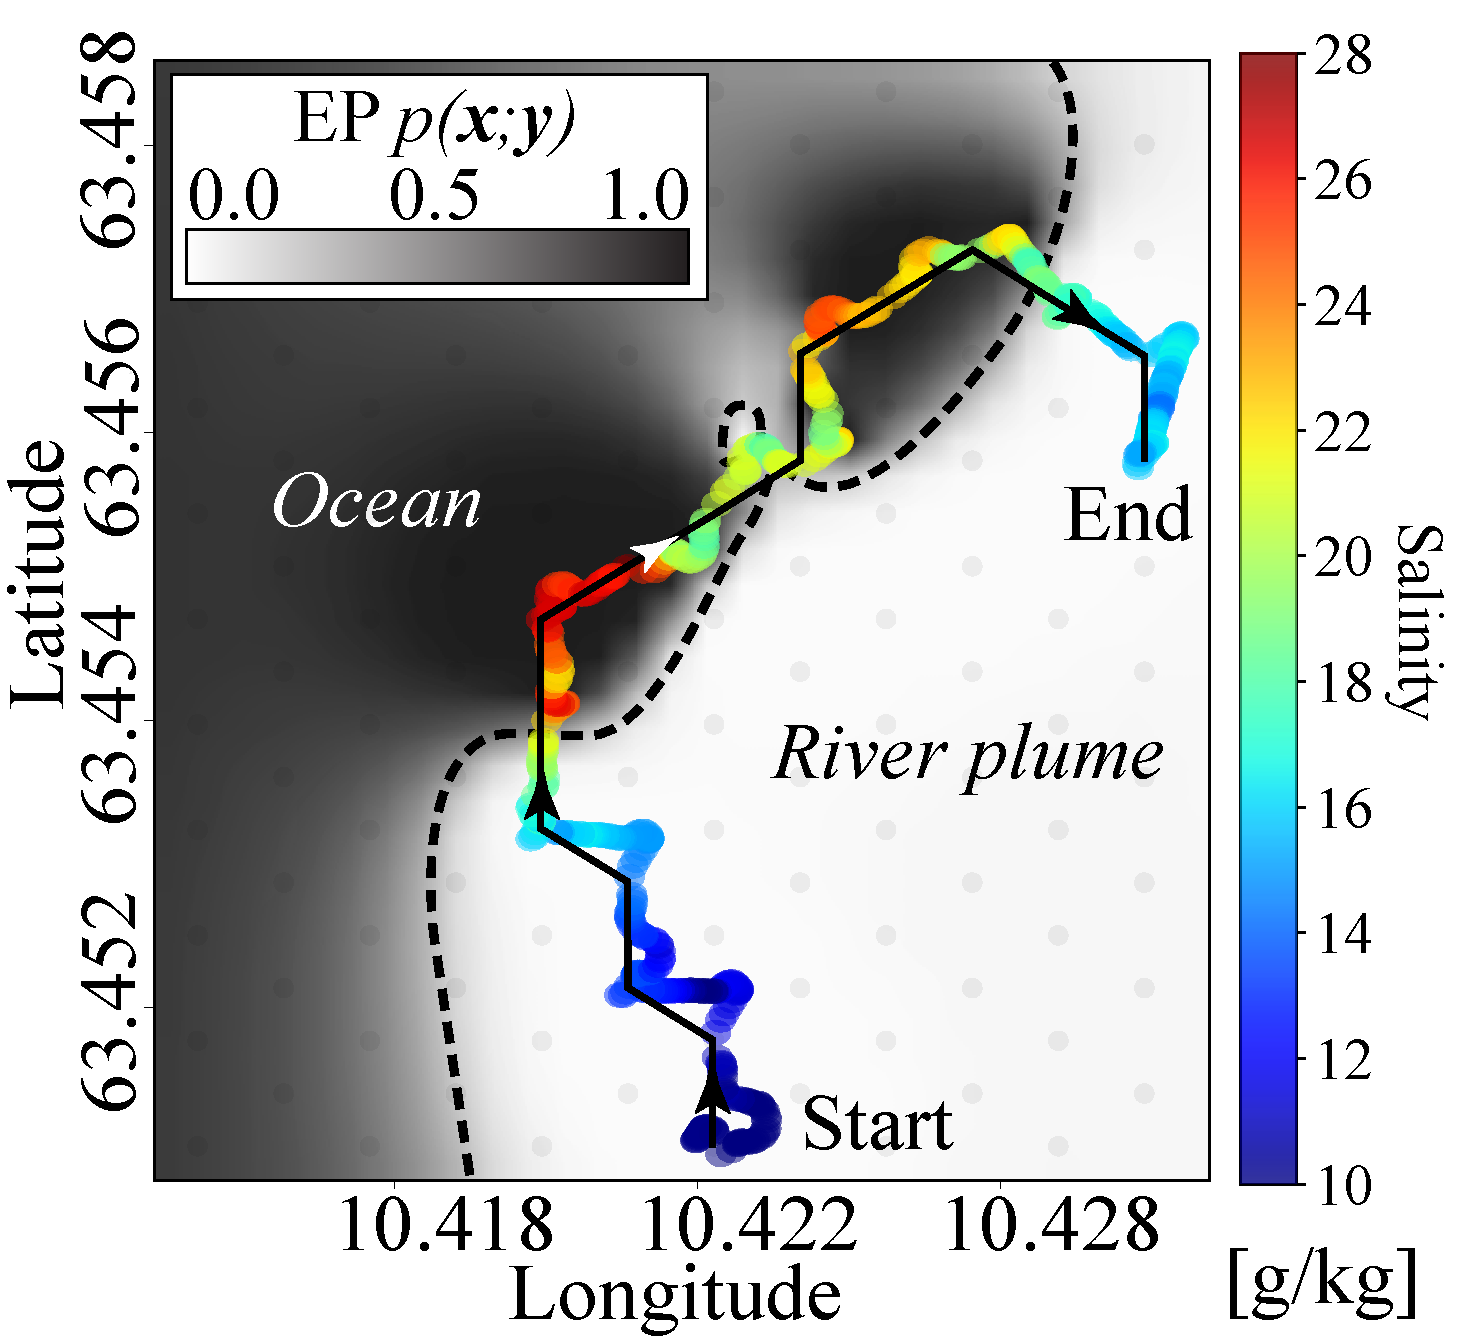
\includegraphics[height=0.40\textwidth]{Figures/field-trials/auv1_es_sal_ep.pdf}\label{fig:res1}}
\hspace{0.2cm}
\subfigure[Survey 2]{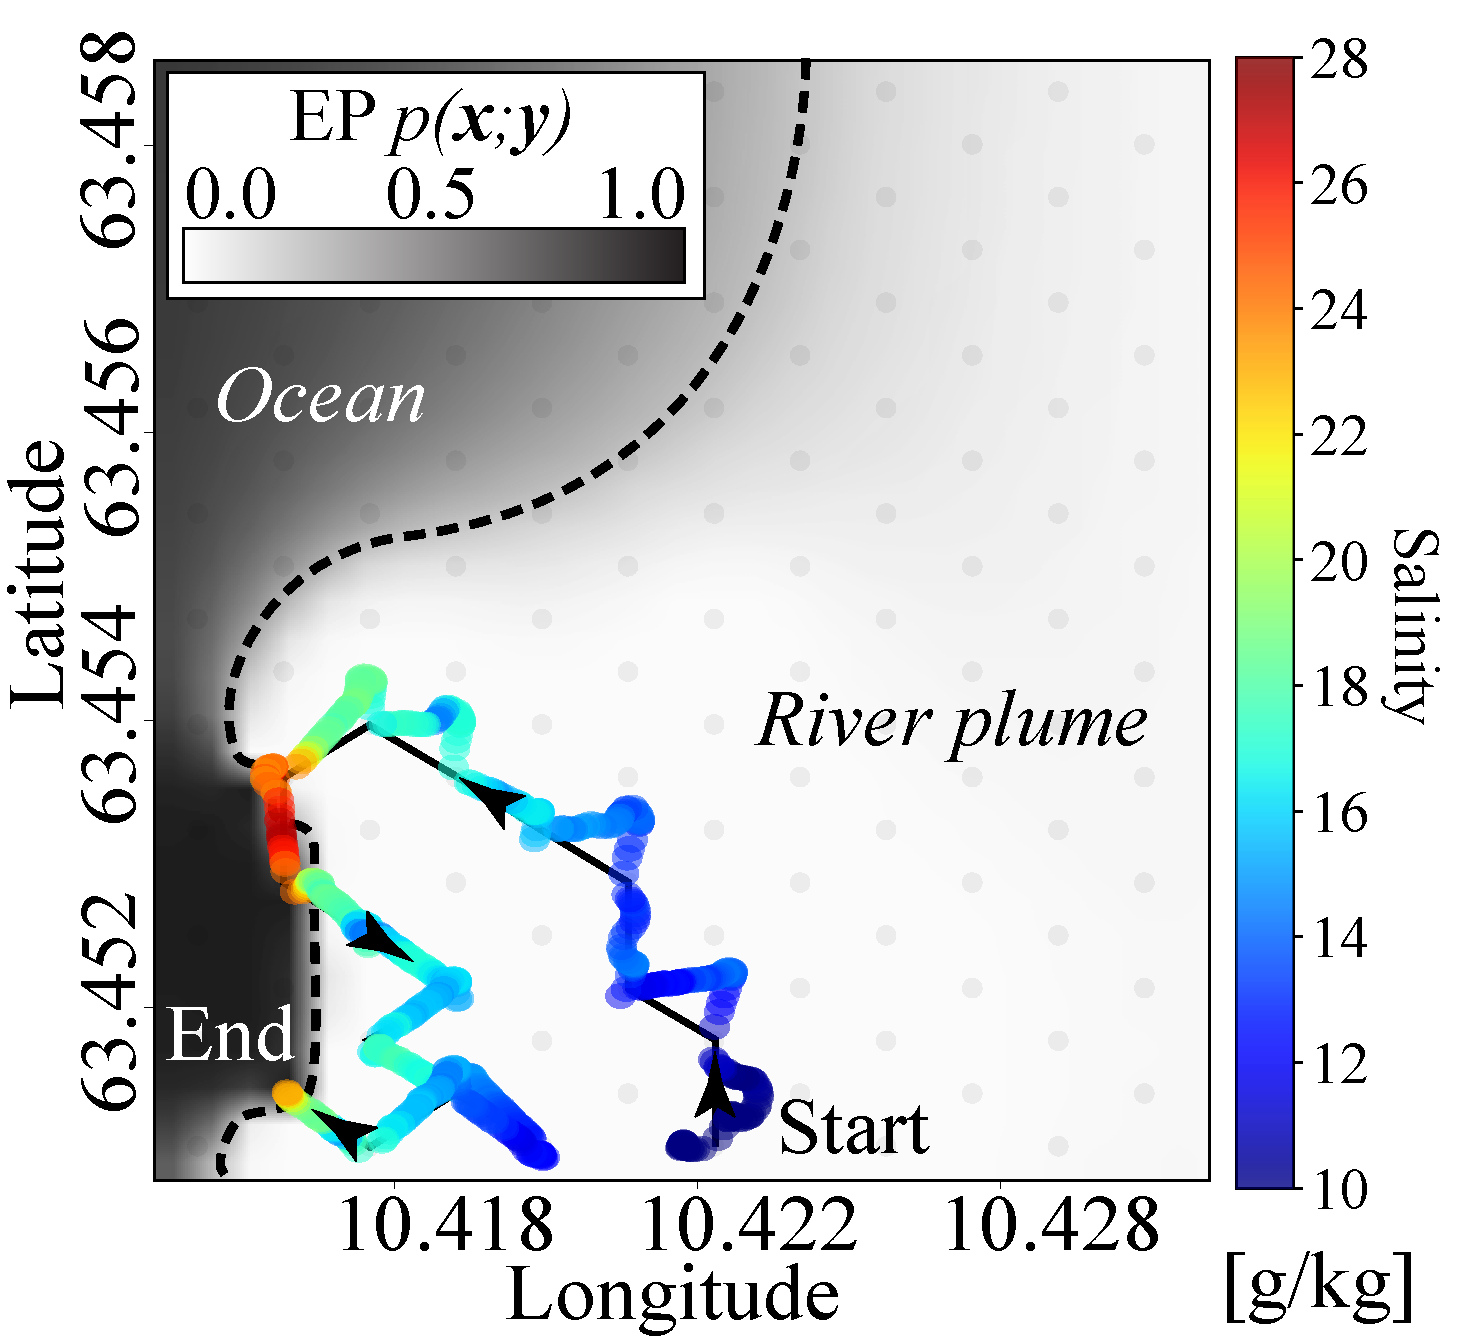
\includegraphics[height=0.40\textwidth]{Figures/field-trials/auv4_es_sal_ep.pdf}\label{fig:res2}}

%\subfigure[ES for Survey 1]{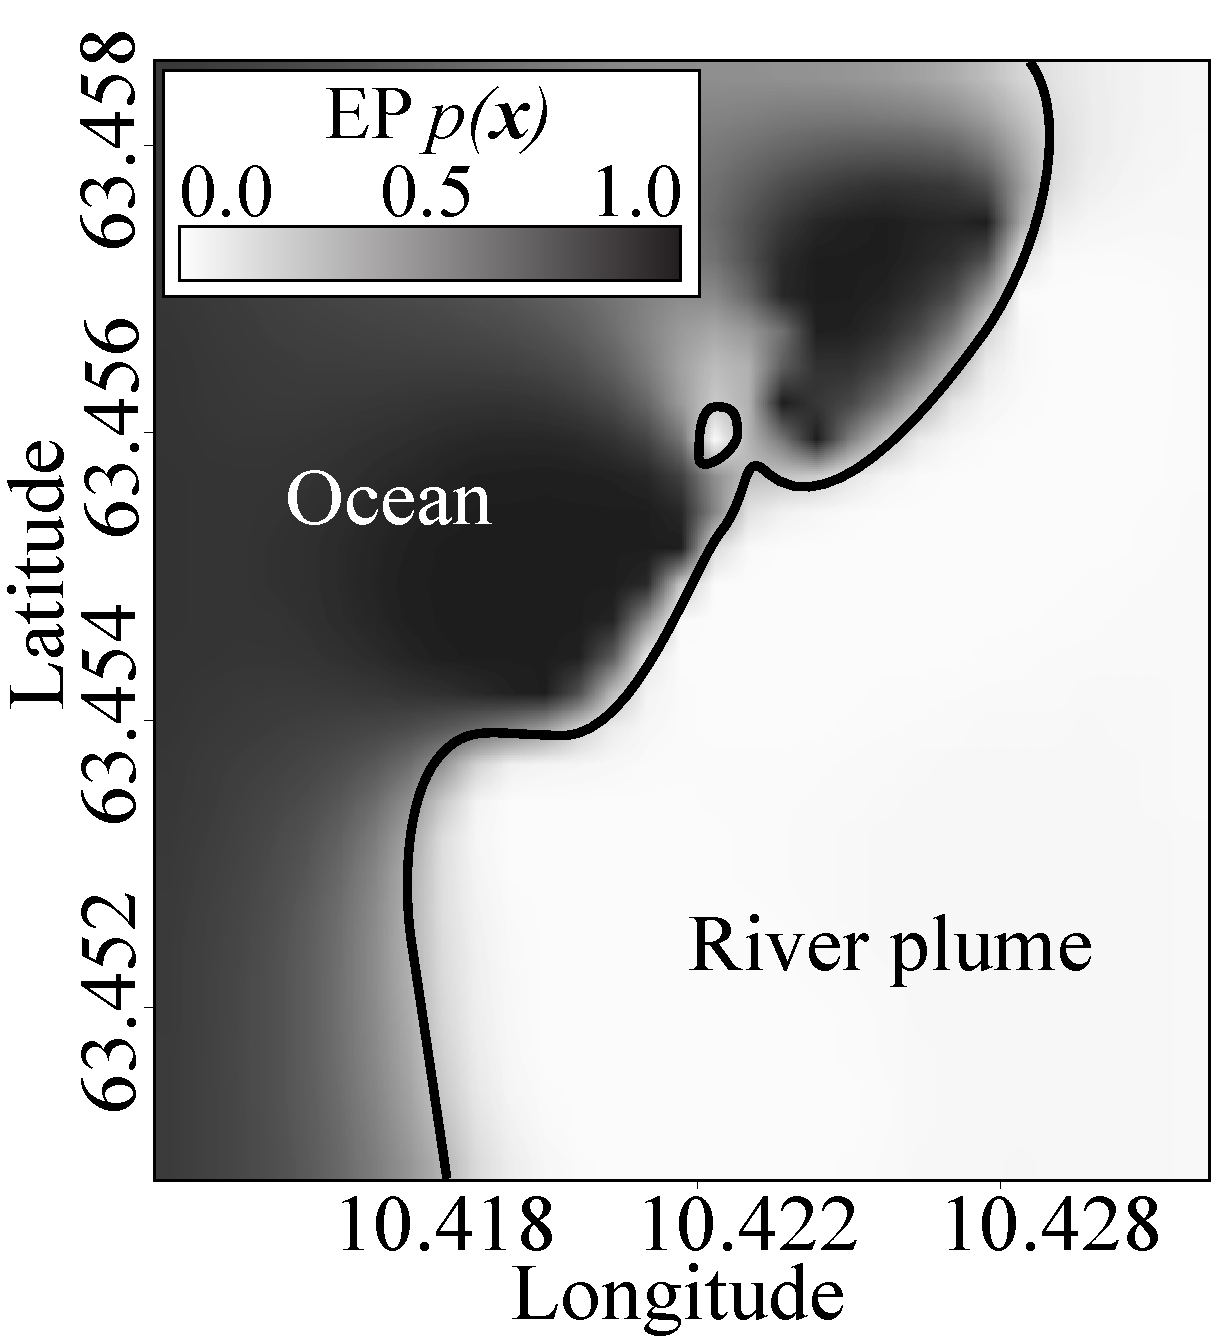
\includegraphics[height=0.41\textwidth]{Figures/field-trials/ep_1.pdf}\label{fig:res3}}\hspace{0.4cm}
%\subfigure[ES for Survey 2]{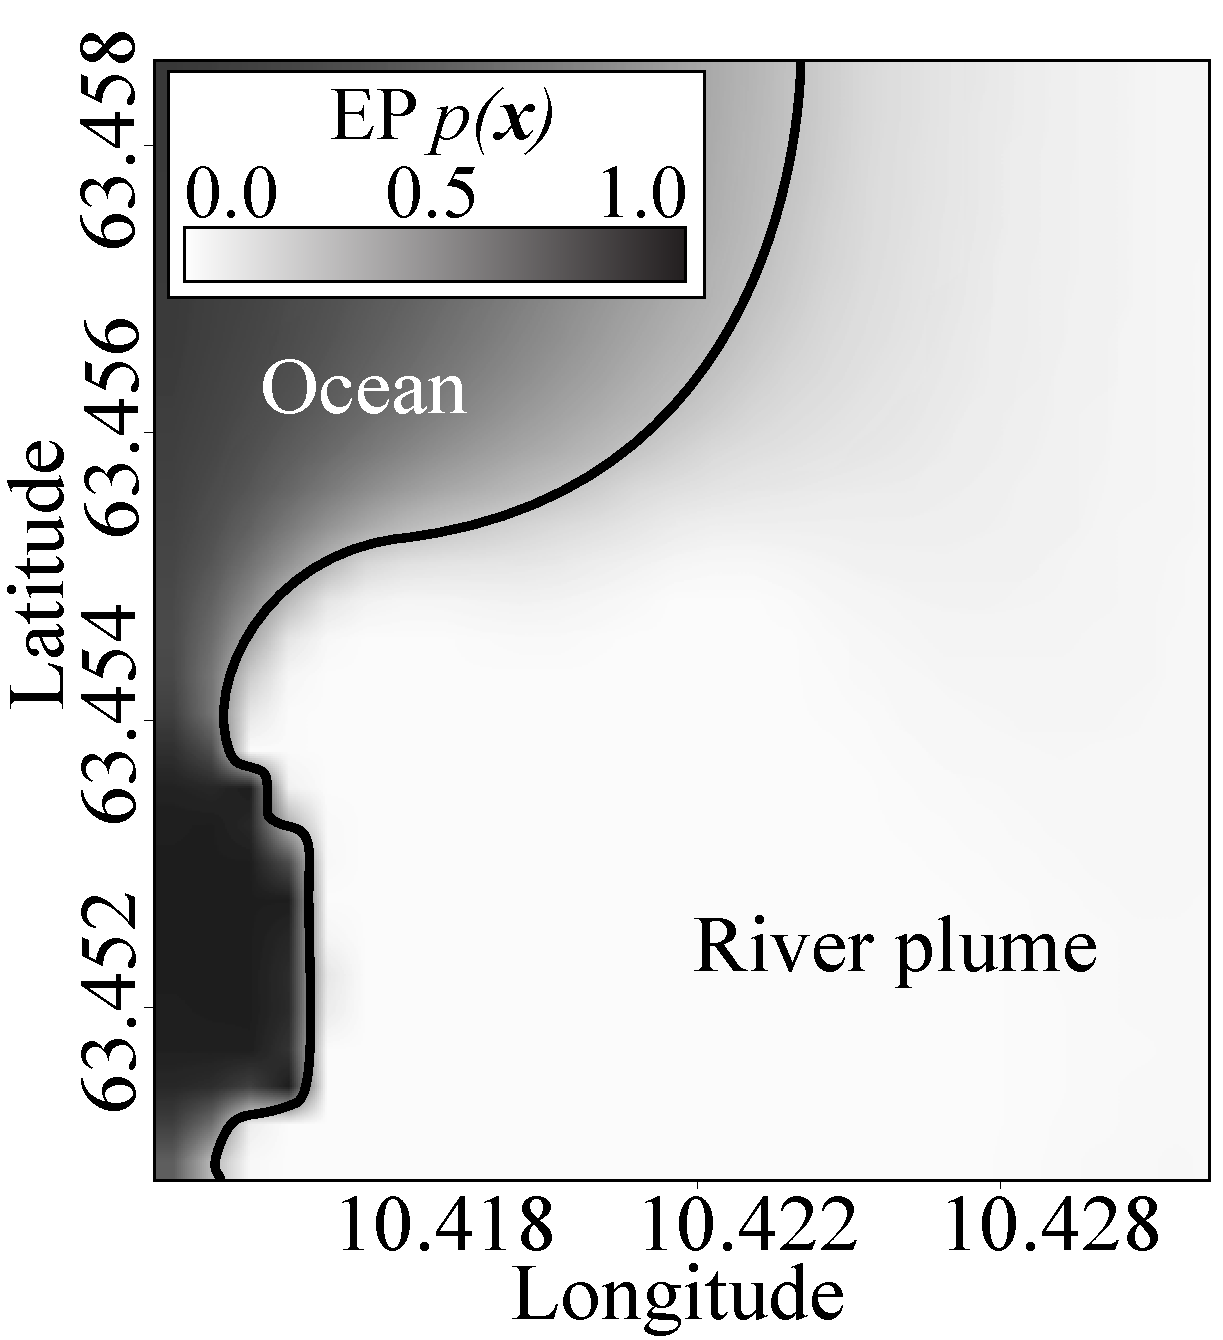
\includegraphics[height=0.41\textwidth]{Figures/field-trials/ep_4.pdf}\label{fig:res4}}
\caption{Results from mapping the Nidelva river, Trondheim, Norway
  over two survey missions. \ref{fig:map} shows an overview of the
  survey area overlaid with the AUV path in black and dashed
  line. Note the shaded region indicating a typical frontal
  region. \ref{fig:res_both} shows the collected temperature data as
  colored trails. Note waypoint 5 (WP5) which indicates where the two
  surveys diverge. \ref{fig:res1} and \ref{fig:res2} shows the
  collected salinity data overlaid on the final EP, which indicate the
  AUVs statistical impression of the front. For both missions the
  temperature and salinity data correspond with an indication of the
  EP front. \kc{Might want to indicate when the surveys (dates) were
    conducted so people can understand the variability in the EP with
    respect to time.}}
\label{fig:results}
\end{figure*}

\subsection{Results}

Two surveys missions (1 and 2), were run successively from 11:00 AM to
01:00 PM, with a short break in between. The resulting path of the
selected waypoints are shown in the map in Fig. \ref{fig:map}, both
within the expected frontal region (shaded pink). The recorded
temperatures are shown as colored trails in Fig. \ref{fig:res_both},
clearly indicating the temperature difference between fjord and
riverine waters. The salinity data are then shown separately, overlaid
with the estimated EP for each survey in Fig. \ref{fig:res1} and
\ref{fig:res2}.

Both surveys successfully estimated and navigated the separation zone,
crossing the frontal boundary multiple times. As conditions changed
slightly between the two surveys, the resulting path (after waypoint
5) is shown to deviate. Survey 1 continued northwards, tracking the
north-eastern portion of the front, while Survey 2 turned west,
mapping the south-western region.

The final predictions of the front location, represented by
conditional EPs in Fig. \ref{fig:res1} and \ref{fig:res2} as dashed
lines, correspond with one another. In both surveys they yield a
picture of the front being to the west in the southern portions of the
region and gradually bending off toward the north east. The amount of
exploration done by Survey 1 is greater than Survey 2. In Survey 1,
the AUV obtained more detail by going north from waypoint 5, while
Survey 2, coming close to the survey area borders in the south-western
corner, obtained a poorer understanding of the northern parts. A
look-ahead strategy might identify and discourage such choices.

%\begin{figure}[!h] 
% \centering 
%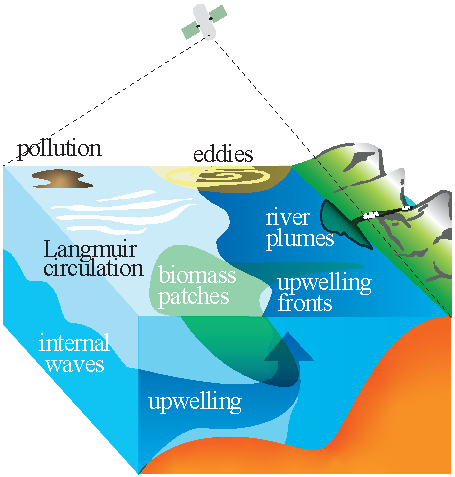
\includegraphics[width=0.48\textwidth]{Figures/envir_ocean.pdf}
%\caption{Ocean observation is moving away from %single-ship sampling
%towards more collaborative networked operations in %order to resolve
%the numerous processes and their interaction.} %\label{fig:envir}
%\end{figure}
%\newpage
\section{Closing remarks}\label{sec:concl_disc}

This work builds on a multidisciplinary effort combining statistical
methods with robotic surveying techniques for oceanographic
applications. We show how observation practices can gain efficiency
and accuracy from the development of statistical techniques for spatial monitoring. We further demonstrate the
opportunities available for real-time multivariable spatial
data gathering and analysis onboard autonomous platforms, which
statisticians can exploit to create general-purpose toolkits for
similar applications.

In particular, we derive and show results for characterizing phenomena
connected to the properties of water masses. The characterization of
uncertainties in random sets is extended with new results for the expected integrated Bernoulli variance
reduction achieved by spatial sampling designs. This is
provided in closed-form for the situation with a static design, and
then extended to the adaptive situation. The sequential derivations
provide new insights into efficient applications of adaptive data collection,
as demonstrated in our application.

The case study consider the upper water column in the river plume, represented by a two dimensional grid. Extensions to three-dimensional domains are not methodologically different, but the operation must likely approximate calculations by integrating terms only in the vicinity of the autonomous vehicle \citep{fossum18b}. We did not consider any temporal effects, which would be
relevant on a larger time scale. We consider the extension to
spatio-temporal modeling as future work, and envision that
advection-diffusion equations could be useful in this kind of modeling
\citep{sigrist2015stochastic,richardson2017sparsity}. For more complex oceanographic
phenomena, the methods will need to be extended to non-Gaussian
phenomena, possibly feature-based mixtures of Gaussian processes which could still be
run onboard and augmented by dynamical models. 

The spatial-statistical design criterion building on random sets is
relevant in our setting with different water properties. 
We show
mathematical generality beyond the expected integrated Bernoulli variance, for instance that of volume uncertainties which is possibly more relevant, but requires more computational resources.
Such criteria could be particularly useful in other oceanographic settings of algal-blooms, anoxic
zones or open water fronts \cite{costa19}.
Of course, other criteria
are also relevant for instance, hybrid or multi-attribute criteria
that could balance goals of exploration and exploitation in this
situation. Equally, such techniques have significant use cases in
downstream decision-making, with policy makers and regulators who need
to make difficult decisions related to fish farming or other marine
resource operations, and value of information analysis
\citep{Eidsvik:15} could be used to evaluate whether
information is likely to result in improved decision-making.

\kc{How about talking
  about removing any grids or waypoints altogether?}

In our context the myopic strategy perform rather well, and for computational reasons we did not go in depth on the dynamic program solution. There has been much creative work on finite horizon optimization in the robotics literature including probabilistic road maps and rapidly-exploring random trees \citep{karaman2011sampling}, but their statistical properties are not yet clear.
It is equally interesting to
explore the additional flexibility that can be gained by having
multiple vehicles co-temporally exploring a spatial or spatio-temporal
domain \citep{ferreira2019advancing}. Such an approach would enable
concurrent sampling in different parts of the space, or opportunities
to move in parallel to best capture the excursion set.
The sometimes conflicting topics of autonomy and communication have caught much interest in control engineering lately \citep{zolich2019survey}, and statistical evaluations could contribute in the future. In our context, autonomy is highlighted, and this is reflected in our modeling and computational assumptions. With the possibilities of wifi communication to a mother-ship at waypoints, more advanced modeling and computational routines are of course possible, but with new challenges related to design and planning for when and where the communication should occur. 


\section*{Acknowledgements}

TOF acknowledges support from the Centre for Autonomous Marine
Operations and Systems
(AMOS)\footnote{\url{https://www.ntnu.edu/amos}}, Center of
Excellence, project number 223254, and the Applied Underwater Robotics
Labortatory (AURLab). JE and KR acknowledge support from Norwegian
research council (RCN), project number 305445. CT and DG acknowledge
support from the Swiss National Science Foundation, project number
178858.

%\begin{supplement}
%\sname{Supplement A}\label{suppA}
%\stitle{Title of the Supplement A}
%\slink[url]{http://www.e-publications.org/ims/support/dowload/imsart-ims.zip}
%\sdescription{Dum esset rex in
%accubitu suo, nardus mea dedit odorem suavitatis. Quoniam confortavit
%seras portarum tuarum, benedixit filiis tuis in te. Qui posuit fines tuos}
%\end{supplement}

% == Adding references
\footnotesize
\bibliographystyle{imsart-nameyear}
\bibliography{ref}


\section*{Appendix}

\begin{propo}
    \label{propo1}
%Under technical conditions to be precised, $\mu(\es)$ possesses moments or arbitrary order and these can be expressed for any $r\geq 1$ as
For a measurable random field $\gp$ and a locally finite measure $\mes$ on $D$, $\mes(\es)$ is a random variable and for 
any $r\geq 1$,
\begin{equation*}
\begin{split}
\mathbb{E}[\mes(\es)^r]
&=\int_{D^{r}} \jointExcuProb
\productMeasure
,
\end{split}
\end{equation*}

where the product measure is denoted as
$\nu^{\otimes}:=\bigotimes_{i=1}^r \nu$.
%Note that we will use boldface to denote concatenated variables. % TO RELOCATE
Here $\gp$ is defined on $D$, and for
$\bm{u}=\left(u^{(1)}, ..., u^{(r)}\right)\in D^r$, $\gp[\bm{u}]=\left(\gp[u^{(1)}], ...,
\gp[u^{(r)}]\right)\in \mathbb{R}^{\no r}$.
\medskip

In the particular case where $\gp$ is a multivariate Gaussian random field
%and denoting the mean and covariance matrix of $\gp[\bm{u}]$ by $\meanUU\in\mathbb{R}^{p\times r}$ and $\covUU$, respectively,
we have
\begin{align*}
\jointExcuProb = \mathcal{N}_{\no r}(T^r; \meanUU, \covUU),
\end{align*}
where $\mathcal{N}_{\no r}(\cdot ; \meanUU, \covUU)$ is the Gaussian measure on $\mathbb{R}^{\no r}$ with mean $\meanUU$ 
and covariance matrix $\covUU$, respectively defined blockwise by
%where both are defined blockwise by
\begin{align*}
\meanUU&=\begin{pmatrix}\mu(u^{(1)})\\ \vdots\\ \mu(u^{(r)})\end{pmatrix}
\in \mathbb{R}^{\no r}, \\
\text{and } \covUU &= \begin{pmatrix}
\cov(\gp[u^{(1)}], \gp[u^{(1)}]) & \dots & \cov(\gp[u^{(1)}],
\gp[u^{(r)}])\\
\vdots & & \vdots\\
\cov(\gp[u^{(r)}], \gp[u^{(1)}]) & \dots & \cov(\gp[u^{(r)}],
\gp[u^{(r)}])\\
\end{pmatrix}\in \mathbb{R}^{pr\times pr},
\end{align*}
each of the $r\times r$ blocks of the latter matrix being itself a (cross-)covariance matrix of dimension $\no \times 
\no$.
%dimensional Gaussian random vector.
Assuming further that $\covUU$ is non-singular, the probability of interest can be formulated in terms of the $\no 
r$-dimensional Gaussian probability density function
$\varphi_{\no  r}(\cdot;~\meanUU, \covUU)$ as
%$\varphi_{\no \times r}$ as
%$\bm{u}\in D^r$ such that $\gp[\bm{u}]$ be non-degenerate, the integrand can be expressed in terms of the $r \times \no$-dimensional Gaussian distribution, namely
%cumulative distribution function, namely
\begin{equation*}
\begin{split}
&\jointExcuProb
=
\int_{T^r} \varphi_{\no  r}\left(\bm{v};
    ~\meanUU, \covUU\right)
    \mathrm{d}\bm{v},
\end{split}
\end{equation*}
In the particular orthant case with $\T=(-\infty, t_1] \times \dots \times (-\infty, t_{r}]$,
the latter probability directly writes in terms of the multivariate Gaussian
cumulative distribution, % with mean $\meanUU$ and covariance matrix $\covUU$,
this time by the way without requiring $\covUU$ %the latter
to be non-singular:
\begin{equation*}
\begin{split}
\jointExcuProb
&=
\varPhi_{\no r}\left(\bm{t};~\meanUU, \covUU\right),
\end{split}
\end{equation*}
where we have used the notations
$t=(t_1,\dots,t_{\no}%,..., t_1, ..., t_p
)\in\mathbb{R}^{\no}$, $1_{r}=(1,\dots,1)\in \R^{r}$, and
$\bm{t}=1_{r}\otimes \bm{t}=(t_1,\dots,t_{\no},\dots,t_1,\dots,t_{\no})
\in \R^{\no r}$.
\end{propo}
\begin{proof}
That $\mes(\es)$ defines indeed a random variable follows from Fubini's theorem
relying on the joint measurability of
$(\x, \omega) \to \mathbbm{1}_{\es(\omega)}(\x)$,
%= \mathbf{1}_{\xi_{\x}(\omega) \in T}$ and Fubini's theorem.
itself inherited from the assumed measurability for
$(\x, \omega) \to \gp[\x](\omega)$ and $T$, respectively. From there, following the steps of Robbins' theorem \cite{Robins1944}, we find that
\begin{equation*}
\begin{split}
\mathbb{E}[\mes(\es)^{r}]
&=\mathbb{E}\left[\left(\int_{D} \mathbbm{1}_{\gp[u] \in T} ~d\mes(u) \right)^{r} \right]
=\mathbb{E}\left[ \prod_{i=1}^{r} \left(
        \int_{D} \mathbbm{1}_{\gp[\uu^{(i)}] \in T} ~d\mes(\uu^{(i)})
\right) \right] \\
&
=
%\mathbb{E}\left[
%\int_{D^{r}}
%\prod_{i=1}^{r}
%\mathbf{1}_{\gp[\uu^{(i)}] \in T}
%\productMeasure
%\right]
%=
\mathbb{E}\left[
\int_{D^{r}}
\mathbbm{1}_{\gp[\uu^{(1)}] \in T,\dots, \gp[\uu^{(r)}]  \in T}
\productMeasure
\right]
%\\
%&=\int_{D^{r}} \mathbb{E}\left[\mathbf{1}_{\gp[\bm{u}] \in T^r} \right] \productMeasure \\
%&
=\int_{D^{r}}
\jointExcuProb
\productMeasure.
\end{split}
\end{equation*}
The rest consists in expliciting the probability of $T\times \dots \times T$ under the multivariate Gaussian distribution of
$\left(\gp[u^{(1)}], \dots,  \gp[u^{(r)}] \right)$.
\end{proof}

The propositions below provide formulae for computations of expectations of moments of multivariate gaussian CDFs.

\begin{propo}
    \label{propo2}
Let $p, q, h \geq 1$, $a \in \R^p$, $B \in \R^{p\times q}$,
and $\covN, \covV$ be two covariance matrices in
$\R^{p\times p}$ and $\R^{q\times q}$, respectively.
Then, for $V \sim \mathcal{N}_{q}(0_q, \covV)$,
\begin{equation*}
\mathbb{E}\left[ \varPhi_{p}\left( a + BV; \covN \right)^h \right]
=
\varPhi_{ph}
\left(
    \bm{a}
;~
\bm{\Sigma}
\right),
\end{equation*}
where the vector $\bm{a} \in \R^{p h}$ is defined as
$\bm{a} := 1_h\otimes a = 
\left(a, \dots , a
\right)'$
 and the $p h\times p h$ covariance matrix is given by
 $\bm{\Sigma} := 
1_h 1_h'\otimes B\covV B' + I_h\otimes \covN$.
\end{propo}

\begin{remark}
In blockwise representation, $\bm{\Sigma}$ can be expressed as follows:
\begin{align*}
% \bm{\Sigma}&=
\begin{pmatrix}
    \covN & &\\
        & \ddots &\\
        &   & \covN
\end{pmatrix}
+
\begin{pmatrix}
B\covV B' & \dots & B\covV  B'\\
\vdots & & \vdots\\
B\covV B' & \dots & B\covV B'\\
\end{pmatrix}
\end{align*}
\end{remark}

\begin{proof}
By definition of $\Phi_{p}$, for $N\sim \mathcal{N}_{p}(0_{p},\covN)$,
$$
\mathbb{P}(N\leq a + BV | V)
=
\varPhi_{p}\left( a + BV; \covN \right).
$$
Now for $\varPhi_{p}\left( a + BV; \covN \right)^h$, provided that the probability space is sufficiently large to accomodate $h$ independent Gaussian random vectors $N_i\sim \mathcal{N}_{p}(0,\covN)$ (which is silently assumed here), using the former equality delivers
$$
\varPhi_{p}\left( a + BV; \covN \right)^h
=
\prod_{i=1}^h \mathbb{P}(N_i\leq a + BV | V).
$$
Now by independence of the $N_i$'s we obtain the joint conditional probability
$$
\prod_{i=1}^h \mathbb{P}(N_i\leq a + BV | V)
=
\mathbb{P}(N_1\leq a + BV, \dots, N_h\leq a + BV| V),
$$
whereof, by virtue of the law of total expectation,
\begin{equation*}
\begin{split}
\mathbb{E}\left[ \varPhi_{p}\left( a + BV; \covN \right)^h \right]
&=\mathbb{E}\left[\mathbb{P}(N_1\leq a + BV, \dots, N_h\leq a + BV| V)\right]\\
&=\mathbb{P}(N_1\leq a + BV, \dots, N_h\leq a + BV)\\
&=\mathbb{P}(W_1 \leq a, \dots, W_h\leq a)\\
&=\varPhi_{ph}
\left(
1_{h} \otimes a
;
(1_{h}1_{h}')\otimes (B\Sigma_{V} B') + 
I_{h}\otimes \covN
\right),
\end{split}
\end{equation*}
where $\mathbf{W}=(W_1,\dots,W_h)$ with $W_i=N_i- BV \ (1\leq i \leq h)$
and the last line follows $\mathbf{W}$ forming a Gaussian vector (by global independence of the $N_i$'s and $V$) and from the definition of $\varPhi_{p h}$. The covariance matrix $\mathbf{\Sigma}$ of $\mathbf{W}$ is obtained by noting that $\operatorname{cov}(W_i,W_j)=B \covV B' + \delta_{ij} \covN \ 
(i,j \in \{1,\dots,h\})$.
%the latter concatenated Gaussian vector is obtained by straightfoward calculation. 
\end{proof}

We now generalize Proposition~\ref{propo2} to the case of multivariate monomials in orthant probabilities with thresholds affine in a common Gaussian vector.
%Namely, for monomials of degree $k$, we have.

\begin{propo}
    \label{propo3}
Let $g, p, q\geq 1$, $h_{1},\dots, h_{g}\geq 1$ with $H=\sum_{i=1}^g h_i$, $a_{i} \in \R^{p}$, $B_{i}\in \R^{p \times q}$, and covariance matrices $\covN_i \in \R^{p \times p}$ $(1\leq i \leq g)$. Then, for any covariance matrix $\covV \in \R^{q\times q}$ and $V\sim\mathcal{N}_{q}(0_q,\covV)$,
    \begin{equation}
    \mathbb{E}\left[ \prod_{i=1}^{g} \varPhi_{p}\left(a_i + B_{i}V; \covN_{i} \right)^{h_i} \right]
    =
\varPhi_{p H}
\left(
    \bm{a}
;
\mathbf{\Sigma}
\right),
\end{equation}
with $\bm{a}=(1_{h_1}\otimes a_1, \dots, 1_{h_g}\otimes a_{g}) \in \R^{p H}$
and $\mathbf{\Sigma}\in \R^{p H \times p H}$ is defined blockwise by $(\Sigma_{i,j})_{i,j \in \{1,\dots, g\}}$ where, for any $i,j \in \{1,\dots, g\}$, %the blocks are given by 
\begin{equation}
\Sigma_{i,j}=
(1_{h_{i}}1_{h_{j}}')\otimes (B_{i}\Sigma_{V} B_{j}') + \delta_{i,j}(I_{h_{i}}\otimes \covN_{i}) \in \R^{p h_{i} \times p h_{j}}.
\end{equation}
\end{propo}

\begin{remark}
Using blockwise representation for the blocks themselves delivers %$\bm{\Sigma}$ can be expressed as follows
\begin{equation*}
%    \bm{\Sigma} = \begin{pmatrix}
%        \Sigma_{11} & & \Sigma_{1g}\\
%        & \ddots &\\
%        \Sigma_{g1}&   & \Sigma_{gg}
%\end{pmatrix},~
\Sigma_{ij} =
\begin{pmatrix}
B_i\Sigma_{V} B_j' & \dots & B_i\Sigma_{V} B_j'\\
\vdots & & \vdots\\
B_i\Sigma_{V} B_j' & \dots & B_i\Sigma_{V} B_j'\\
\end{pmatrix}
+
\delta_{ij}
\begin{pmatrix}
    \covN_i & &\\
        & \ddots &\\
        &   & \covN_i
\end{pmatrix}%\in\mathbb{R}^{lh_i\times lh_j}
\end{equation*}
Here each $\Sigma_{ij}$ is made of $h_i$ times $h_j$
(vertically/horizontally) $p \times p$ sub-blocks, hence possesses $ph_i$ lines and $ph_j$ columns.
\end{remark}

\begin{proof}
    The proof relies (again) heavily on the fact that, by definition of $\Phi_{p}$, for any covariance matrix $\covN \in \R^{p \times p}$, $a\in \R^p$, $B\in \R^{p \times q}$, and $N\sim \mathcal{N}_{p}(0_{p},\covN)$,
    $$
    \mathbb{P}(N\leq a + BV | V)
    =
    \varPhi_{p}\left( a + BV; \covN \right).
    $$
In particular, for globally independent $N_{i,j} \sim \mathcal{N}_{p}(0_{p},\covN_i)$ $(1\leq j \leq h_i, 1\leq i \leq g)$,
\begin{equation*}
\begin{split}
\prod_{i=1}^{g} \varPhi_{p}\left(a_i + B_{i}V; \covN_{i} \right)^{h_i}
&=
\prod_{i=1}^{g}
\prod_{j=1}^{h_{i}}
\mathbb{P}(N_{i,j}\leq a_i + B_i V | V)\\
&=\mathbb{P}(N_{1,1}\leq a_1 + B_1 V, \dots, N_{g,h_{g}}\leq a_g + B_g V | V),
\end{split} 
\end{equation*}
so that, by the law of total expectation,
    \begin{equation*}
    \begin{split}
    \mathbb{E}\left[ \prod_{i=1}^{g} \varPhi_{p}\left(a_i + B_{i}V; \covN_{i} \right)^{h_i} \right]
=
\mathbb{P}(W_{1} \leq 1_{h_{1}} \otimes a_1, \dots, W_{g} \leq 1_{h_{g}} \otimes a_g)
    \end{split}
    \end{equation*}
where
$W_{1}=(N_{1,1}- B_1 V, \dots, N_{1,h_{1}}- B_1 V), 
W_{2}=(N_{2,1}- B_2 V, \dots, N_{2,h_{2}}- B_2 V), 
\dots, W_{g}=(N_{g,1}- B_g V, \dots, N_{g,h_{g}}- B_g V)$. Noting that $\mathbf{W}=(W_1,\dots, W_g)$ is a centred $p H$-dimensional Gaussian random vector, we finally obtain that
    \begin{equation*}
\begin{split}
\mathbb{E}\left[ \prod_{i=1}^{g} \varPhi_{p}\left(a_i + B_{i}V; \covN_{i} \right)^{h_i} \right]
=
\varPhi_{p H}\left(\bm{a};\mathbf{\Sigma}\right),
    \end{split}
\end{equation*}
with $\bm{a}=(1_{h_{1}} \otimes a_1, \dots, 1_{h_{g}} \otimes a_g)$ and $\bm{\Sigma}=(\operatorname{cov}(W_i,W_j))_{i,j \in \{1,\dots, g\}}$.
\end{proof}

Those two general results allow us to derive simple expressions for the expected effect of the inclusion of new datapoints on the $\ibv$ (Proposition \ref{propo_eibv}) and on the $\emv$ (Proposition \ref{propo_emv}) for which we provide proofs below.


\begin{proof}{(Proposition \ref{propo_eibv})}
Applying Tonelli-Fubini followed by the law of total
expectation first delivers
\begin{equation*}
\begin{split}
\eibv_{[n]}(\bm{x})
&=\int_{D}
\currentExp{\futureProba{\gp[\uu]\in
        T}(1-\futureProba{\gp[\uu]\in T})} d\mes(u) \\
&=\int_{D} \varPhi_{\no}\left(\bt;
~\futureMean{\uu},
\futureCov{u,u}\right) d\mes(u)\\
&-\int_{D} \currentExp{
    \varPhi_{\no}\left(\bt;
    ~\futureMean{\uu},
    \futureCov{u,u}\right)^2
}
d\mes(u), 
\end{split}
\end{equation*}
%
where $\futureCov{u,u}$ denotes the $\no \times \no$ covariance matrix between all $\no$
responses at point $u$ conditional on the first $n+1$ observation batches.
Now, by using co-kriging update formulae and our shortcut notation for the CDF of centred
multivariate Gaussian vectors, we observe that
\begin{equation*}
\begin{split}
%\mathbb{E}_{n}[\left(
&\varPhi_{\no}\left(\bt;~\futureMean{\uu}, \futureCov{u, u}\right) 
%\right)^2]
\\
=&
\varPhi_{\no}\left(\bt-\futureMean{\uu}; \futureCov{u, u}\right) \\
=&
\varPhi_{\no}\left(\bt-\currentMean{\uu}-\lambda_{[n+1,n+1]}(u)^T(\gp[\bm{x}_{n+1}]
-\currentMean{\bm{x}_{n+1}}), \futureCov{u, u}\right) \\
=&
\varPhi_{\no}\left(a + BV, \futureCov{u, u}\right),
\end{split}
\end{equation*}
with $a=\bt-\currentMean{\uu}$, %+\lambda_{[n+1,n+1]}(u)^T\currentMean{\bm{x}_{n+1}}$,
$B=-\lambda_{[n+1,n+1]}(u)^T$
and $V=\gp[\bm{x}_{n+1}]-\currentMean{\bm{x}_{n+1}}$.
Applying Proposition~\ref{propo2} then delivers that
%
\begin{equation*}
\begin{split}
&\currentExp{
    \varPhi_{\no}\left(\bt;~\futureMean{\uu}, \futureCov{u, u}\right)^2 
}
%\\
=\varPhi_{2\no}
\left(
\left(
\begin{matrix}
\bt-\currentMean{\uu}\\
%\vdots \\ 
%\vdots \\ 
%\vdots \\ 
\bt-\currentMean{\uu}
\end{matrix}
\right);
\mathbf{\Sigma}_{[n]}(\uu)
\right),
\end{split}
\end{equation*}
with $\mathbf{\Sigma}_{[n]}(\uu)$ as in the formulation of the proposition. This completes the proof.
\end{proof}


\begin{proof}{(Proposition \ref{propo_emv})}
\begin{equation*}
\begin{split}
\eemv_{[n]}(\bm{x})
%\operatorname{Var}[\mes(\es)]
&=\int_{D^2} 
\varPhi_{2\no}
\left(
(\bt, \bt); \mu((u,v)), 
K((u,v),(u,v))
\right) 
\
\mathrm{d}\mes^{\otimes} %\mes 
%\productMeasure 
(u,v)\\
&-\currentExp{\left( \int_{D} \varPhi_{\no}\left(\bt;\mu_{[n+1]}(u), K_{[n+1]}(u)\right) d\mes(u) \right)^2}.
\end{split}
\end{equation*}
The second term can be worked out in semi-analytical form by writing it as
%
\begin{equation*}
\begin{split}
%\eemv_{[n]}(\bm{x})
%\operatorname{Var}[\mes(\es)]
&\int_{D^2} 
\currentExp{
\varPhi_{\no}\left(\bt;\mu_{[n+1]}(u), K_{[n+1]}(u)\right)
\varPhi_{\no}\left(\bt;\mu_{[n+1]}(v), K_{[n+1]}(v)\right)
}
\
\mathrm{d}\mes^{\otimes} %\mes 
%\productMeasure 
(u,v)\\
=&
\int_{D^2} 
\currentExp{
    \varPhi_{\no}\left(a_1+B_1 V; C_1\right)
    \varPhi_{\no}\left(a_2+B_2 V; C_2\right)
}
\
\mathrm{d}\mes^{\otimes} %\mes 
%\productMeasure 
(u,v),\\
\end{split}
\end{equation*}
and expanding the integrand (for fixed $n$, $\uu, \vv$) as
\begin{equation*}
\begin{split}
&
\currentExp{
    \varPhi_{\no}\left(\bt;\mu_{[n+1]}(u), K_{[n+1]}(u)\right)
    \varPhi_{\no}\left(\bt;\mu_{[n+1]}(v), K_{[n+1]}(v)\right)
}\\
=&
\currentExp{
    \varPhi_{\no}\left(a_1+B_1 V; C_1\right)
    \varPhi_{\no}\left(a_2+B_2 V; C_2\right)
}
\end{split}
\end{equation*}
with $V=\gp[\bm{x}_{n+1}]-\currentMean{\bm{x}_{n+1}} \sim \mathcal{N}(0_{q_{n+1}},k_{[n]}(\bm{x}_{n+1},\bm{x}_{n+1}))$ and $a_1=\bt-\currentMean{\uu}$,
$B_1=-\lambda_{[n+1,n+1]}(\uu)^T$, $a_2=\bt-\currentMean{\vv}$, $B_2=-\lambda_{[n+1,n+1]}(\vv)^T$.
\end{proof}



% AOS,AOAS: If there are supplements please fill:
%\begin{supplement}[id=suppA]
%  \sname{Supplement A}
%  \stitle{Title}
%  \slink[doi]{10.1214/00-AOASXXXXSUPP}
%  \sdatatype{.pdf}" 
%  \sdescription{Some text}
%\end{supplement}

% === Not used
% After reviews: - This is moved to Section 2.1. 

%Traditional data collection at sea has typically been based on static
%buoys, Lagrangian floats, or ship-based methods, with significant
%logistical limitations that directly impact coverage and sampling
%resolution. Modern methods using satellite remote-sensing provide
%large-scale coverage but have limited resolution, are limited to
%sensing the surface of the ocean, and are impacted by cloud cover. The
%advent of robust mobile robotic platforms \citep{Bellingham07} has
%resulted in significant contributions to environmental monitoring and
%sampling. In particular, autonomous underwater vehicles (AUVs), have
%advanced the state of sampling and consequently have made robotics an
%integral part of ocean observation; our previous work has contributed
%to this effort \citep{das11b,Das2015,fossum18b,fossuminformation}. Other ¤ %statistical work in the oceanographic domain include \cite{wikle2013modern}
%focusing on hierarchical statistical models; \cite{sahu2008space},
%studying spatio-temporal models for sea surface temperature and
%salinity data; and \cite{mellucci2018oceanic} looking at the
%statistical prediction of features using an underwater glider.

%\begin{itemize}
%
%\item Full numerical ocean models cannot provide accurate results
%  online if run on robotic sensing platforms, as onboard computers
%  cannot deliver the computational power required. Hence statistical
%  proxy models of the environment must be used for learning where to sample.
%
%\item With limited available information about the state of the ocean, there is substantial value in reacting to
%  information obtained from measurements taken in-situ. This
%  acquired information must be assimilated into statistical models that
%  can be used to inform decisions on where to sample
%  sequentially.%\emph{in-situ}; this is usually referred to as the \emph{adaptivity gap} \citep{ause2008phd}.
%
%\item For sampling problems related to environmental sensing, the
%  number of choices (i.e. locations, trajectories, and candidate
%  designs) is enormous, creating a
%  trade-off between optimization (finding the most resource-efficient
%  design to collect necessary data) and computability (arriving at a
%  solution in reasonable time). To successfully resolve features, this
%  trade-off has to be considered in development and practice.
%
%\end{itemize}

%Addressing this, the combination of statistical tools and robotic platforms is a
%natural symbiosis which enables information-based sensing. Central to
%this is the ability to model spatially-correlated variables and
%provide formal measures of uncertainty. Our formulation is based on
%Gaussian Processes (GPs) as they allow efficient implementation 
%and evaluation in real time onboard a robotic platform.

%Sampling can, in this context, not simply be distributed evenly ---along simple transects or ``lawn-mover" patterns--- but must instead be prioritized to relevant regions to ensure it is cost-effective while providing adequate coverage and resolution of the area of scientific interest.

%While the focus has often been on
%biological and anthropogenic impact from micro-plastics to
%pollution, biological oceanographers have focused intently on studying
%micro-organisms at the base of the human food web. These organisms are
%critically impacted by the changing dynamics in the upper water-column,
%especially in coastal zones which are complex and often hard to observe
%in space and time. By studying the bio-geochemical processes in the
%upper water-column scientists can measure the impact of change, natural
%or anthropomorphic, and provide an informed opinion to policy makers to
%effect changes in preserving the environment. However, the challenge of 
% The pressure on marine resources is growing and increased accuracy,
% resolution, and persistent monitoring of the oceans is crucial for
% long-term sustainable management. 

% A
% sustained focus on prioritized and efficient data collection strategies
% have therefore started to emerge. The advent of marine robotic
% platforms, especially

% provided means to execute this prioritization through the capacity of
% autonomy and data-driven sampling, where data collection in principle
% can be optimized. These capabilities have made

% of the emerging sensing practice for ocean science, allowing scientists
% to increase the observational efficiency and resolution beyond what was
% previously possible. But how should a robotic platform, such as an AUV,
% effectively prioritize and identify important regions for sampling? The
% answer to this question relates to 

% , and
% the application domain is clearly an arena where statisticians can
% contribute.
% There has recently been some statistical attention in oceanography:

%From an oceanographic perspective, interesting regions are usually directly tied to a distinct phenomena that is of scientific interest. Each phenomenon can in turn be characterized by a set of process specific conditions expressed through different measures of key environmental variables, such as temperature or salinity. One such measure is the gradient, that can be associated with a number of important processes, such as the vertical location of the thermocline and pycnocline, location of upwelling systems, vertical mixing, eddies, fronts, and currents \cite{sverdrup2006}, as well as distribution, growth, and accumulation of biological activity \cite{SatOceanSoci00, Ryan2014}. These gradients create boundaries separating the ocean into process specific regions which are of profound interest to both identify and map effectively. Quantification of gradient features is therefore a much needed competence in robotic sampling.
\end{document}

